%----------
%   IMPORTANTE
%----------

% Esta plantilla está basada en las recomendaciones de la guía "Trabajo fin de Grado: Escribir el TFG", que encontrarás en http://uc3m.libguides.com/TFG/escribir
% contiene recomendaciones de la Biblioteca basadas principalmente en estilos APA e IEEE, pero debes seguir siempre las orientaciones de tu Tutor de TFG y la normativa de TFG para tu titulación.

\newcommand{\vbus}{V_{\text{bus}}}
\newcommand{\vout}{V_{\text{out}}}
\newcommand{\vin}{V_{\text{in}}}
\newcommand{\vdiodo}{V_{\text{D}}}
\newcommand{\rdson}{R_{\text{DS,ON}}}
\newcommand{\Tswitch}{T_{\text{sw}}}
\newcommand{\fswitch}{f_{\text{sw}}}
\newcommand{\Ton}{T_{\text{on}}}
\newcommand{\Toff}{T_{\text{off}}}
\newcommand{\deltaILon}{\Delta i_{\text{L,on}}}
\newcommand{\deltaILoff}{\Delta i_{\text{L,off}}}
\newcommand{\deltaIL}{\Delta i_\text{L}}
\newcommand{\iLmedia}{I_{\text{L,media}}}
\newcommand{\Lmin}{L_{\text{min}}}
\newcommand{\IhistSup}{I_{\text{hys,sup}}}
\newcommand{\IhistInf}{I_{\text{hys,inf}}}
\newcommand{\Imax}{I_{\text{max}}}
\newcommand{\tsense}{t_{\text{sense}}}


% ESTA PLANTILLA ESTÁ BASADA EN EL ESTILO IEEE


%----------
%	CONFIGURACIÓN DEL DOCUMENTO
%----------

\documentclass[12pt,twoside,openright]{report} % fuente a 12pt
\raggedbottom
\usepackage{comment}
% MÁRGENES: 2,5 cm sup. e inf.; 3 cm izdo. y dcho.
\usepackage[
a4paper,
vmargin=2.5cm,
hmargin=3cm
]{geometry}
\usepackage[dvipsnames]{xcolor}

\newenvironment{bloqueRevisar}
    {\color{red}} % Lo que hace al empezar el bloque
    {\ignorespacesafterend} % Lo que hace al terminar

% INTERLINEADO: Estrecho (6 ptos./interlineado 1,15) o Moderado (6 ptos./interlineado 1,5)
\renewcommand{\baselinestretch}{1.15}
\parskip=6pt
\usepackage{amsmath}
% DEFINICIÓN DE COLORES para portada y listados de código
\usepackage[table]{xcolor}
\definecolor{azulUC3M}{RGB}{0,0,102}
\definecolor{gray97}{gray}{.97}
\definecolor{gray75}{gray}{.75}
\definecolor{gray45}{gray}{.45}
\usepackage{physics}
% Soporte para GENERAR PDF/A --es importante de cara a su inclusión en e-Archivo porque es el formato óptimo de preservación y a la generación de metadatos, tal y como se describe en http://uc3m.libguides.com/ld.php?content_id=31389625. 

% En la plantilla incluimos el archivo OUTPUT.XMPDATA. Puedes descargar este archivo e incluir los metadatos que se incorporarán al archivo PDF cuando compiles el archivo memoria.tex. Después vuelve a subirlo a tu proyecto. 
\usepackage[a-1b]{pdfx}

% ENLACES
\usepackage{hyperref}
\hypersetup{colorlinks=true,
	linkcolor=black, % enlaces a partes del documento (p.e. índice) en color negro
	urlcolor=blue} % enlaces a recursos fuera del documento en azul

% EXPRESIONES MATEMÁTICAS
\usepackage{amsmath,amssymb,amsfonts,amsthm}
\usepackage[siunitx]{circuitikz} % Para circuitos electrónicos
\usepackage{tikz} % Base de dibujos

% Codificación caracteres
\usepackage{txfonts} 
\usepackage[T1]{fontenc}
\usepackage[utf8]{inputenc}

% Definición idioma español
\usepackage[spanish, es-tabla]{babel} 
\usepackage[babel, spanish=spanish]{csquotes}
\AtBeginEnvironment{quote}{\small}

% diseño de PIE DE PÁGINA
\usepackage{fancyhdr}
\pagestyle{fancy}
\fancyhf{}
\renewcommand{\headrulewidth}{0pt}
\rfoot{\thepage}
\fancypagestyle{plain}{\pagestyle{fancy}}

% DISEÑO DE LOS TÍTULOS de las partes del trabajo (capítulos y epígrafes o subcapítulos)
\usepackage{titlesec}
\usepackage{titletoc}
\titleformat{\chapter}[block]
{\large\bfseries\filcenter}
{\thechapter.}
{5pt}
{\MakeUppercase}
{}
\titlespacing{\chapter}{0pt}{0pt}{*3}
\titlecontents{chapter}
[0pt]                                               
{}
{\contentsmargin{0pt}\thecontentslabel.\enspace\uppercase}
{\contentsmargin{0pt}\uppercase}                        
{\titlerule*[.7pc]{.}\contentspage}                 

\titleformat{\section}
{\bfseries}
{\thesection.}
{5pt}
{}
\titlecontents{section}
[5pt]                                               
{}
{\contentsmargin{0pt}\thecontentslabel.\enspace}
{\contentsmargin{0pt}}
{\titlerule*[.7pc]{.}\contentspage}

\titleformat{\subsection}
{\normalsize\bfseries}
{\thesubsection.}
{5pt}
{}
\titlecontents{subsection}
[10pt]                                               
{}
{\contentsmargin{0pt}                          
	\thecontentslabel.\enspace}
{\contentsmargin{0pt}}                        
{\titlerule*[.7pc]{.}\contentspage}  


% DISEÑO DE TABLAS
\usepackage{multirow} % permite combinar celdas 
\usepackage{caption} % para personalizar el título de tablas y figuras
\usepackage{floatrow} % utilizamos este paquete y sus macros \ttabbox y \ffigbox para alinear los nombres de tablas y figuras de acuerdo con el estilo definido.
\usepackage{array} % con este paquete podemos definir en la siguiente línea un nuevo tipo de columna para tablas: ancho personalizado y contenido centrado
\newcolumntype{P}[1]{>{\centering\arraybackslash}p{#1}}
\DeclareCaptionFormat{upper}{#1#2\uppercase{#3}\par}

% Diseño de tabla para ingeniería
\captionsetup*[table]{
	format=upper,
	name=TABLA,
	justification=centering,
	labelsep=period,
	width=.75\linewidth,
	labelfont=small,
	font=small
}

% DISEÑO DE FIGURAS. 
\usepackage{graphicx}
\graphicspath{{imagenes/}} % ruta a la carpeta de imágenes

% Diseño de figuras para ingeniería
\captionsetup[figure]{
	format=hang,
	name=Fig.,
	singlelinecheck=off,
	labelsep=period,
	labelfont=small,
	font=small		
}

% NOTAS A PIE DE PÁGINA
\usepackage{chngcntr} % para numeración continua de las notas al pie
\counterwithout{footnote}{chapter}

% LISTADOS DE CÓDIGO
% soporte y estilo para listados de código. Más información en https://es.wikibooks.org/wiki/Manual_de_LaTeX/Listados_de_código/Listados_con_listings
\usepackage{listings}

% definimos un estilo de listings
\lstdefinestyle{estilo}{ frame=Ltb,
	framerule=0pt,
	aboveskip=0.5cm,
	framextopmargin=3pt,
	framexbottommargin=3pt,
	framexleftmargin=0.4cm,
	framesep=0pt,
	rulesep=.4pt,
	backgroundcolor=\color{gray97},
	rulesepcolor=\color{black},
	%
	basicstyle=\ttfamily\footnotesize,
	keywordstyle=\bfseries,
	stringstyle=\ttfamily,
	showstringspaces = false,
	commentstyle=\color{gray45},     
	%
	numbers=left,
	numbersep=15pt,
	numberstyle=\tiny,
	numberfirstline = false,
	breaklines=true,
	xleftmargin=\parindent
}

\captionsetup*[lstlisting]{font=small, labelsep=period}
% fijamos el estilo a utilizar 
\lstset{style=estilo}
\renewcommand{\lstlistingname}{\uppercase{Código}}


%BIBLIOGRAFÍA 

% CONFIGURACIÓN PARA LA BIBLIOGRAFÍA IEEE
\usepackage[backend=biber, style=ieee, isbn=false,sortcites, maxbibnames=6, minbibnames=1]{biblatex} % Configuración para el estilo de citas de IEEE, recomendado para el área de ingeniería. "maxbibnames" indica que a partir de 6 autores trunque la lista en el primero (minbibnames) y añada "et al." tal y como se utiliza en el estilo IEEE.

% Añadimos las siguientes indicaciones para mejorar la adaptación del estilos en español
\DefineBibliographyStrings{spanish}{%
	andothers = {et\addabbrvspace al\adddot}
}
\DefineBibliographyStrings{spanish}{
	url = {\adddot\space[En línea]\adddot\space Disponible en:}
}
\DefineBibliographyStrings{spanish}{
	urlseen = {Acceso:}
}
\DefineBibliographyStrings{spanish}{
	pages = {pp\adddot},
	page = {p.\adddot}
}

\addbibresource{referencias.bib} % llama al archivo referencias.bib en el que deberá estar la bibliografía utilizada


%-------------
%	DOCUMENTO
%-------------

\begin{document}
\pagenumbering{roman} % Se utilizan cifras romanas en la numeración de las páginas previas al cuerpo del trabajo
	
%----------
%	PORTADA
%----------	
\begin{titlepage}
	\begin{sffamily}
	\color{azulUC3M}
	\begin{center}
		\begin{figure}[H] %incluimos el logotipo de la Universidad
			\makebox[\textwidth][c]{
\includegraphics[width=16cm]{logo_UC3M.png}}
		\end{figure}
		\vspace{2.5cm}
		\begin{Large}
			Grado Universitario en Ingeniería Electrónica Industrial y Automática\\			
			 2025-2026\\ %Indica el curso académico
			\vspace{2cm}		
			\textsl{Trabajo Fin de Grado}
			\bigskip
			
		\end{Large}
		 	{\Huge Diseño, modelado e implementación de un circuito conmutado para la protección por sobre-corriente}\\
		 	\vspace*{0.5cm}
	 		\rule{10.5cm}{0.1mm}\\
			\vspace*{0.9cm}
			{\LARGE Álvaro Villalta Vázquez}\\ 
			\vspace*{1cm}
		\begin{Large}
			Tutora\\
			Cristina Fernández Herrero\\
			Lugar y fecha de presentación prevista\\
		\end{Large}
	\end{center}
	\vfill
	\color{black}
	% SI NUESTRO TRABAJO SE VA A PUBLICAR CON UNA LICENCIA CREATIVE COMMONS, INCLUIR ESTAS LÍNEAS. ES LA OPCIÓN RECOMENDADA.
	
\includegraphics[width=4.2cm]{creativecommons.png}\\ %incluimos el logotipo de Creative Commons
	Esta obra se encuentra sujeta a la licencia Creative Commons \textbf{Reconocimiento - No Comercial - Sin Obra Derivada}
	\end{sffamily}
\end{titlepage}

\newpage %página en blanco o de cortesía
\thispagestyle{empty}
\mbox{}

%----------
%	RESUMEN Y PALABRAS CLAVE
%----------	
\renewcommand\abstractname{\large\bfseries\filcenter\uppercase{Resumen}}
\begin{abstract}
\thispagestyle{plain}
\setcounter{page}{3}
	
	% ESCRIBIR EL RESUMEN AQUÍ
	
	\textbf{Palabras clave:}
	% Escribir las palabras clave aquí
	
	\vfill
\end{abstract}
	\newpage % página en blanco o de cortesía
	\thispagestyle{empty}
	\mbox{}


%----------
%	DEDICATORIA
%----------	
\chapter*{Dedicatoria} % \chapter* evita que aparezca en el índice

\setcounter{page}{5}
	
	% ESCRIBIR LA DEDICATORIA AQUÍ	
		
	\vfill
	
	\newpage % página en blanco o de cortesía
	\thispagestyle{empty}
	\mbox{}
	

%----------
%	ÍNDICES
%----------	

%--
% Índice general
%-
\tableofcontents
\thispagestyle{fancy}

\newpage % página en blanco o de cortesía
\thispagestyle{empty}
\mbox{}

%--
% Índice de figuras. Si no se incluyen, comenta las líneas siguientes
%-
\listoffigures
\thispagestyle{fancy}

\newpage % página en blanco o de cortesía
\thispagestyle{empty}
\mbox{}

%--
% Índice de tablas. Si no se incluyen, comenta las líneas siguientes
%-
\listoftables
\thispagestyle{fancy}

\newpage % página en blanco o de cortesía
\thispagestyle{empty}
\mbox{}


%----------
%	MEMORIA
%----------	
\clearpage
\pagenumbering{arabic} % numeración con números arábigos para el resto de la memoria.	

\chapter{Introducción}
Los limitadores de corriente de enclavamiento (en adelante, LCL, por sus siglas en inglés, Latching Current Limiter) son circuitos de protección empleados en los sistemas de distribución de energía, ubicados habitualmente entre el bus de potencia principal y las cargas secundarias del sistema \cite{noauthor_latching_nodate}.

A diferencia de un fusible tradicional, la función principal de un LCL no es únicamente interrumpir el circuito ante un fallo. Su cometido es limitar la corriente demandada por la carga a un valor máximo prefijado en caso de que se produzca una sobrecarga o un cortocircuito. Si esta condición anómala persiste de forma continuada durante un intervalo de tiempo específico (conocido como tiempo de trip-off), el LCL procede entonces a la desconexión segura de la carga para proteger el bus de potencia. Esta alta fiabilidad y previsibilidad lo han convertido en un estándar indispensable en la industria aeroespacial.

Además de su robustez, la capacidad de aislar fallos de manera controlada y la posibilidad de rearmar la carga posteriormente (por ejemplo, mediante telecomandos), expanden su utilidad a numerosos ámbitos. Su implementación resulta idónea para todo tipo de aplicaciones terrestres críticas y entornos de laboratorio que demanden una gestión de potencia segura, monitorizada y tolerante a fallos.

\section{Problemática actual}
Históricamente, las topologías tradicionales de LCLs han empleado transistores MOSFET de canal P (en adelante, P-MOS) como elementos limitadores de corriente. La principal ventaja de esta elección radica en la simplicidad de su circuito de control: el driver gobierna el transistor aplicando un voltaje en puerta inferior al del bus.

Sin embargo, esta arquitectura presenta severas limitaciones de rendimiento y escalabilidad. En primer lugar, los dispositivos P-MOS presentan inherentemente una resistencia de canal mayor que los de canal N (N-MOS) para una misma tensión nominal. Esto supone, durante el funcionamiento nominal, mayores pérdidas por conducción lo que puede obligar a paralelizar semiconductores en aplicaciones de altas corrientes, incrementando el volumen y la complejidad del sistema.

El problema más crítico, no obstante, se encuentra durante un evento de sobrecarga. Para limitar la corriente al valor de referencia, el LCL tradicional fuerza al P-MOS a operar en modo activo (zona lineal), mediante la variación del valor de la resistencia interna. En este estado, el transistor estará soportando un voltaje el cual podrá llegar hasta el valor de la tensión del bus, provocando que el semiconductor disipe una enorme potencia durante el tiempo de temporización elegido (trip-off).
En consecuencia, se provocará un incremento drástico y rápido de su temperatura lo cual restringirá la fiabilidad del dispositivo. Además, este estrés térmico dificultará el escalado del LCL hacia buses de tensión sobre 100 o 120 voltios por la escasez de P-MOS en el mercado que puedan soportar estos niveles de voltaje manteniendo niveles reducidos de resistencia de canal.

\section{Solución propuesta}
 Con el objetivo de superar las limitaciones térmicas y de escalabilidad que presentan los transistores P-MOS, en la década de los 90 la evolución de los interruptores de estado sólido convergió hacia la adopción de los transistores MOSFET de canal N (N-MOS) para las topologías high-side. 

La ventaja de los N-MOS radica en su propia física: la movilidad de los electrones en los N-MOS es considerablemente mayor a la de los huecos de los P-MOS, lo que en la práctica supone una resistencia de conducción (RDSON) en torno a 3 veces menor a la de un MOSFET de canal P similar \cite{tim_skovmand_micropower_1993}.

A pesar de esta superioridad ampliamente conocida desde hace muchos años, el uso de los N-MOS como interruptor high-side se ha visto obstaculizada por la complicación inherente a la excitación del mismo pues el voltaje en la puerta debe ser superior a la de la fuente, el cual es el voltaje del bus.
Tradicionalmente, para generar el voltaje necesario para la puerta era necesario el uso de un convertidor DC-DC aislado, el cual, debido al volumen que ocupaba, su coste elevado y su complejidad llevaba a desestimar su uso en numerosos diseños.
Por otro lado, las técnicas de bootstrap, como veremos en el capítulo de diseño, resultan inviables en los limitadores de corriente de enclavamiento por estar, en condiciones nominales, el ciclo de trabajo al 100\%, provocando la descarga del condensador al no existir una conmutación que permita recargarlo \cite{tim_skovmand_micropower_1993}.

El punto de inflexión para la generalización de los N-MOS data de principios de la década de los 90, momento en el que la industria logra integrar de forma monolítica, es decir, en un único chip de silicio, circuitos de bomba de carga (charge pump). La integración de los circuitos de bomba de carga supuso un antes y un después, pues permitía elevar el voltaje usando únicamente condensadores e interruptores en la placa, permitiendo así polarizar la puerta del N-MOS y mantenerlo encendido indefinidamente sin fuentes de alimentación externas \cite{noauthor_ltc1155_nodate} , \cite{noauthor_max1614_nodate}. 

Controladores como el LTC1155 \cite{noauthor_ltc1155_nodate}, diseñado para remplazar los P-MOS en buses de potencia, o el MAX1614 \cite{noauthor_max1614_nodate}, consiguieron que la arquitectura high-side basada en N-MOS se estandarizase. 

Apoyándonos en esta evolución tecnológica, el presente trabajo propone el diseño y validación de un limitador de corriente de enclavamiento (LCL) utilizando un N-MOS operando en una topología reductora, tomando como referencia los fundamentos teóricos propuestos por López \textit{et al.} \cite{lopez_antuna_diseno_2024}. Empleando esta arquitectura el transistor estará trabajando en conmutación durante la limitación de corriente, disminuyendo de forma drástica las pérdidas de conducción y, por tanto, mitigando el estrés térmico al que se ve sometido el semiconductor en comparación con los esquemas tradicionales que emplean un P-MOS de forma lineal.  

\section{Objetivos del trabajo}

Como se ha presentado en los anteriores puntos, las topologías tradicionales de limitadores de corriente de enclavamiento (LCL) que emplean MOSFET de canal P se enfrentan a grandes limitaciones por la disipación de potencia debido a la operación en zona lineal durante la sobrecorriente. Para solventar este problema y reducir el estrés térmico del semiconductor, este proyecto propone el empleo de una topología en la que la limitación se lleve a cabo a través de un transistor de canal N en conmutación. Basándonos en esta idea, el presente Trabajo de Fin de Grado persigue los siguientes propósitos.
 
\begin{itemize}
    \item \textbf{Objetivo principal:} Diseñar, simular y validar de forma experimental un Limitador de Corriente de Enclavamiento (LCL) en conmutación basado en tecnología N-MOS, demostrando la mejoría que supone respecto a topologías tradicionales de limitación lineal.
    
    \item \textbf{Objetivos específicos:}
    \begin{itemize}
        \item \textbf{Establecer el marco teórico:} Analizar el estado del arte de los LCL, justificando la motivación para su uso históricamente y la transición de dispositivos P-MOS a N-MOS, y evaluando el impacto de los materiales de banda prohibida ancha (WBG) en ciertas aplicaciones. 
        \item \textbf{Diseñar la etapa de potencia y control:} Seleccionar y dimensionar de forma teórica la topología óptima, incluyendo el diseño y justificación de la inductancia, la frecuencia de conmutación y el lazo de control por histéresis (temporizador y medida de corriente).              
        \item \textbf{Evaluar el sistema mediante simulación:} Modelar el circuito mediante la herramienta de simulación PSIM utilizando componentes ideales y, tras la selección y justificación de los componentes comerciales seleccionados, incorporar los parásitos para predecir el comportamiento real.         
        \item \textbf{Construir y validar el prototipo:} Implementar físicamente el diseño de una placa de circuito impreso (PCB) y comparar los resultados experimentales visibles en el osciloscopio frente a las simulaciones teóricas. 
        \item \textbf{Desarrollar una metodología de escalado:} Definir una estrategia de dimensionado que sistematice el recálculo de los componentes para adaptar el diseño a diferentes niveles de tensión de bus, corrientes nominales y tiempo de disparo. 
    \end{itemize}
\end{itemize}








\chapter{Situación actual}

El siguiente capítulo establece el marco teórico necesario para el desarrollo del presente trabajo de fin de grado. Durante las próximas secciones se realizará un recorrido por los limitadores de corriente de enclavamiento analizando su origen conceptual, su evolución y la adaptación a distintos sectores. Asimismo, se examinará la evolución tecnológica vivida por los dispositivos semiconductores, justificando las topologías tradicionales a través de las limitaciones físicas de estos componentes, y la necesidad de evolucionar hacia soluciones basadas en transistores N-MOS.
Finalmente, se presentarán las bases teóricas comparando la limitación en modo lineal frente al empleo del modo conmutado, justificando de esta manera la topología empleada en el proyecto. 

\section{Origen y fundamentos de los Limitadores de Corriente de Enclavamiento (LCL)}

Los fusibles eléctricos aparecen por primera vez en 1864 \cite{feeo_cables_2023} en forma de alambres con baja temperatura de fusión o placas delgadas con el objetivo de proteger a condensadores de corriente de descarga excesivas, pero no es hasta la década de 1880 cuando, por el gran crecimiento de los sistemas eléctricos, se explota realmente su potencial de protección. 
El principio de funcionamiento del fusible se basa en el uso de un filamento fino fabricado con un material metálico que, ante un aumento de la corriente, aumentará su temperatura debido al efecto Joule, quemándose y abriendo el circuito \cite{sdi_industrial_fusibles_2021}. Esta respuesta no es instantánea y sigue una relación inversa entre la corriente y el tiempo de actuación como se puede ver en las curvas características tiempo-corriente de la figura \ref{fig:I^2vst}.  

\begin{figure}[H]
    \centering
    % Forzamos 10pt para cumplir con la normativa de tu guía
    \fontsize{10}{12}\selectfont 
    \ffigbox[\FBwidth]
    {
        \caption{Ejemplo de comparación entre tiempo de fusión de un fusible y la corriente}
        \label{fig:I^2vst}
    }
    {
        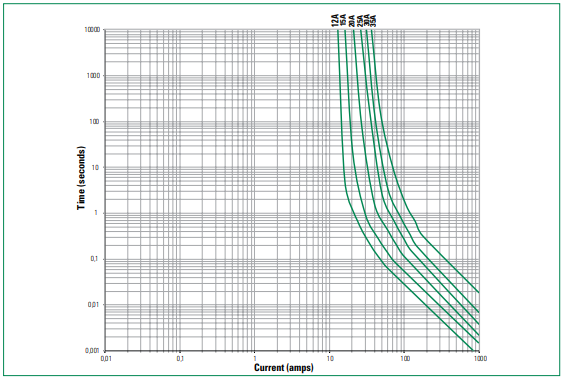
\includegraphics[width=0.7\textwidth]{Ivst.png}
    }
    % Añadimos la fuente requerida por tu guía de TFG
    \vspace{2mm}
    {\raggedleft \textbf{Fuente:} Extraído de la hoja de datos del fusible 0312008.MXP de Littlefuse\cite{littelfuse_inc_fusible_nodate}. \par}
\end{figure}
En ella se observa que el tiempo hasta la fusión disminuye a medida que la magnitud de la corriente aumenta. Por tanto, para sobrecorrientes moderadas los tiempos de respuesta pueden ser de incluso segundos por lo que, antes de aislar la carga, se puede haber producido un daño en la misma. 

Pese a la gran utilidad y revolución que supuso la invención de estos dispositivos debido a la protección que aportaba a un coste muy reducido, pronto surge la necesidad de dotar a ciertos equipos o instalaciones de la posibilidad de rearme del circuito por parte de cualquier usuario sin formación y sin la necesidad de cambiar componentes.

Con esto en mente Thomas Edison describe en 1879 los disyuntores para proteger el cableado de iluminación de sobrecargas, pero es en 1924 cuando Brown, Boveri \verb|&| Cie patentó una versión de tamaño reducido y similar al usado en la actualidad \cite{academia_lab_disyuntor_nodate} \cite{instalaexpert_interruptores_2025}.
Un disyuntor, al igual que los fusibles tradicionales, es un dispositivo que interrumpe de forma automática el flujo de corriente cuando este sobrepasa un límite determinado. Está formado por un interruptor conectado a una pletina bimetálica diseñada para doblarse al superar la corriente el valor para el cual está diseñado\cite{delixi_electric_circuit_2023}.

\begin{figure}[H]
    \centering
    % Forzamos 10pt para cumplir con la normativa de tu guía
    \fontsize{10}{12}\selectfont 
    \ffigbox[\FBwidth]
    {
        \caption{Estructura interna de un disyuntor}
        \label{fig:Disyuntor}
    }
    {
        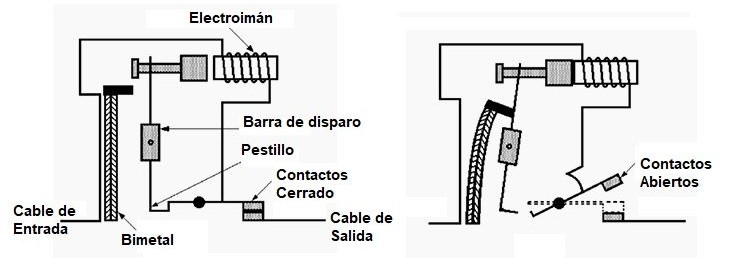
\includegraphics[width=0.7\textwidth]{Disyuntor.jpg}
    }
    % Añadimos la fuente requerida por tu guía de TFG
    \vspace{2mm}
    {\raggedleft \textbf{Fuente:} Extraído de la web Área Tecnológica \cite{noauthor_proteccion_nodate-1}. \par}
\end{figure}

Aunque los disyuntores resolvieron el problema del rearme y la sustitución de componentes debido a su naturaleza mecánica, este mismo factor provoca que tengan limitaciones críticas. No únicamente su tiempo de respuesta de milisegundos es excesivo para ciertos equipos electrónicos sensibles sino que además, en los entornos espaciales sobre los que profundizaremos a lo largo del documento, el desgaste mecánico por vibraciones es reseñable y el arco eléctrico de corriente continua entre la pestaña metálica y el circuito es difícilmente extinguible. Esto es debido a que, mientras que en corriente alterna hay un paso por cero que corta el arco, en corriente continua este mantiene su valor y, por tanto, no se autoextingue, siendo necesario el uso de distancias de aislamiento mucho mayores y, por tanto, repercutiendo en la masa y las dimensiones del sistema.



Como había sucedido con los fusibles anteriormente surge la necesidad de rediseñar el dispositivo para superar barreras térmicas y mecánica. El desarrollo de la electrónica de potencia, disciplina que se centra en la conversión y control de energía eléctrica en niveles de potencia considerables, impulsa la evolución de los disyuntores mecánicos hacia los disyuntores de estado sólido (en adelante, SSCB, por sus siglas en inglés Solid State Circuit Breakers) y los dispositivos encargados de accionarlos, los Controladores de potencia de estado sólido (en adelante, SSPC, por sus siglas en inglés Solid State Power Controller). 
La aparición de estas dos familias de dispositivos supone un antes y un después en el control de circuitos pues, además de ser la base de los convertidores de potencia, son los encargados de remplazar los contactos mecánicos y las pletinas bimetálicas hasta el momento empleados por semiconductores de potencia, siendo los principales los transistores de efecto de campo MOSFET y los transistores bipolares de puerta aislada IGBT.


Estos dispositivos aventajan enormemente a lo disponible hasta la fecha pues, al no constar de partes móviles los tiempos de desconexión se reducen hasta los microsegundos, imposibilita la creación de arcos eléctricos y permite un control más sencillo del circuito. Sin embargo, los SSCB presentan una resistencia en conducción mayor lo que provoca una generación de calor que en los modelos anteriores no es preocupante. Es por ello por lo que se tiende a usar configuraciones en serie o en paralelo que gestionan la limitación. \cite{onsemi_solid-state_nodate}. Otro problema que surge son las interferencias electromagnéticas (EMI) debido a las altas frecuencias de conmutación. 
Ambos problemas se están consiguiendo solucionar mediante el uso de semiconductores de banda ancha (en adelante, WBG, por sus siglas en inglés Wide-bandgap) como el Carburo de Silicio o el Nitruro de Galio que, pese a ser más costosos, tienen características físicas y eléctricas superiores al silicio. \cite{stmicroelectronics_solid_nodate}


Pese a todas las ventajas que presentan, la sensibilidad de estos nuevos circuitos y su apertura prácticamente inmediata tras la detección de una sobrecorriente supone un factor limitante para ciertas aplicaciones en donde no hay posibilidad de rearmar el circuito por no poder acceder a él como es el caso de los satélites, o en aplicaciones donde la conexión de la carga, arranque de motores o carga de bancos de condensadores supone siempre la aparición de transitorios que, pese a ser inofensivos para los dispositivos e incluso anticipados por los fabricantes, provocarían un sobrepaso del umbral y, por tanto, la apertura del circuito y la pérdida de la misión de la carga. 

Es tras esta evolución y en esta situación operacional donde surge la necesidad de crear un circuito capaz de, en caso de detección de sobrecorriente, mantener la carga conectada durante un tiempo predefinido para no abrir el circuito de forma innecesaria debido a un transitorio al conectar o pico de corriente momentáneo, y es, por ende, cuando adquiere importancia el limitador de corriente de enclavamiento o LCL. El valor de este tiempo conocido como \textit{"Trip-off time"} no es un valor seleccionado de forma arbitraria, sino que depende directamente de la capacidad de disipación térmica del semiconductor elegido y la energía máxima que admite la carga.

La ECSS (European Cooperation for Space Standardization) define el LCL como un "dispositivo de protección conmutable y de enclavamiento situado entre una fuente de alimentación y la carga correspondiente, que provoca una desconexión tras alcanzar en su salida un límite de sobrecorriente durante un tiempo de desconexión determinado" [traducción propia]\cite{european_cooperation_for_space_standardization_ecss_latching_nodate}. Como podemos extraer de la definición, el LCL ante una sobrecorriente no desconecta la carga instantáneamente, sino que limita la corriente a un valor seguro para los componentes electrónicos  durante el \textit{Trip-off time} explicado con anterioridad. Por tanto, únicamente si la sobrecorriente persiste una vez este margen de tiempo finaliza se considera que la sobrecorriente es debido a un fallo real y, por tanto, el LCL se enclava en estado abierto, aislando la carga y protegiendo el bus principal. 


Los LCL no deben confundirse con los limitadores de corriente de fallo (FCL por sus siglas en inglés, Fault Current Limiters), ya que mientras un LCL tiene la capacidad de aislar ambas partes del circuito tras un tiempo previamente determinado por la constante de tiempo ${\tau}$ del circuito de temporización, los FCL limitan la corriente a un valor de entre el 10\% y el 25\% de la corriente nominal, sufriendo un estrés térmico mucho mayor y siendo un parámetro clave en el diseño el valor de limitación que debe ser elegido en consonancia con las características y restricciones que impone el semiconductor \cite{marroqui_sempere_david_diseno_nodate}. Sin embargo, la diferencia principal radica en que estos dispositivos no tienen capacidad de enclavamiento, es decir, mantiene el suministro a la carga indefinidamente mientras sufre del estrés térmico por limitar esa corriente.

\section{Evolución tecnológica de los dispositivos semiconductores}

Una vez mostrada la evolución de los sistemas contra sobrecorrientes y establecida la necesidad operativa del LCL para la robustez de los buses de potencial, es necesario analizar el componente que determina el rendimiento que podremos obtener del circuito: el interruptor de estado sólido. Como hemos visto en la sección anterior, la evolución de los protectores está supeditada a los hitos conseguidos en el sector de diseño de los semiconductores de potencia. 
Pese a priorizar la simplicidad de implementación en las primeras arquitecturas empleando dispositivos de canal P, el aumento de los requerimientos de potencia y de las tensiones nominales de los buses en satélites (pasando de 28 V a 100 V) fuerzan a hacer la transición a materiales y polaridades más adecuadas.
En esta sección se analizan tanto las limitaciones del silicio de canal P que han promovido el paso al canal N como las limitaciones del silicio como material, provocando la aparición de nuevos materiales de banda prohibida ancha (WBG) con mayor velocidad de respuesta y eficiencia térmica.


\subsection{Topologías clásicas basadas en canal P (P-MOS)}

Las arquitecturas tradicionales de LCL han empleado a lo largo de los años transistores MOSFET de canal P operando en región lineal durante la sobrecorriente, es decir, se comporta como un elemento resistivo con una curva no lineal y es controlado por tensión. En estas arquitecturas es predominante la colocación \textit{high-side}, donde la fuente del dispositivo se conecta al bus de entrada como podemos ver en la figura \ref{fig:comparativa_mosfet}:

  

\begin{figure}[H]
    \centering
    % Forzamos 10pt para cumplir con la normativa de tu guía
    \fontsize{10}{12}\selectfont 
    \ffigbox[\FBwidth]
    {
        \caption{Comparativa arquitectura \textit{high-side} mediante MOSFET de canal P (izquierda) y canal N (derecha)}
        \label{fig:comparativa_mosfet}
    }
    {
        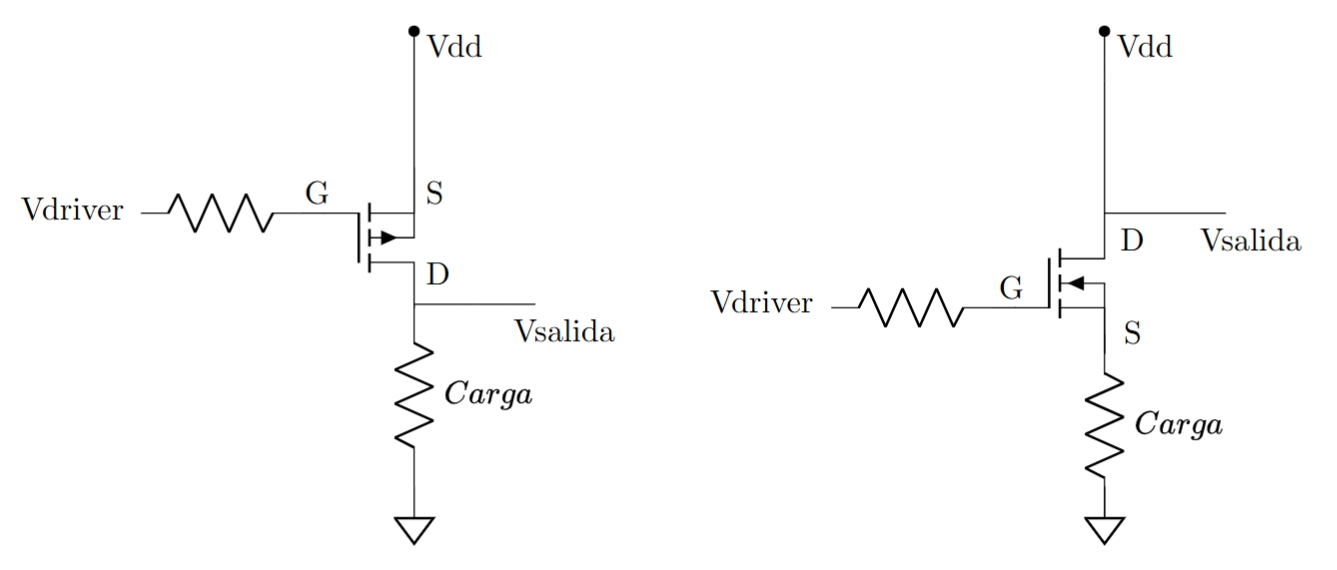
\includegraphics[width=0.8\textwidth]{HighSide.png}
    }
    
    % Añadimos la fuente requerida por tu guía de TFG
    \vspace{2mm}
    {\raggedleft \textbf{Fuente:} Elaboración propia. \par}
\end{figure}



En los MOSFET de tipo P, esta configuración permite regular la corriente de salida mediante la modulación del voltaje entre la puerta y la fuente del semiconductor, estando esta última referenciada respecto al voltaje del bus y, por tanto, pudiendo excitarla mediante un voltaje menor al del bus. Esta característica es la que ha convertido a los P-MOS a lo largo de la historia en la elección predilecta, pues elimina la necesidad de emplear bien fuentes de alimentación aisladas bien circuitos \textit{bootstrap} como es el caso de los N-MOS, simplificando así la arquitectura y reduciendo el coste del dispositivo.
No obstante, durante la limitación de corriente en el modo lineal se produce un gran estrés térmico que puede resultar crítico para el dispositivo. En el intervalo de limitación que ya definimos anteriormente como \textit{trip-off time}, el MOSFET deja de actuar como un interruptor cerrado y, a diferencia de los fusibles, tampoco actúa como un interruptor abierto, sino que actúa como una resistencia que varía para mantener la corriente a un valor constante definido durante el diseño del sistema. Esta corriente será $I_\text{lim}$ y, durante el intervalo de limitación de corriente, el transistor deberá soportar la potencia asociada al paso de esta corriente junto a una caída de tensión similar a la del bus ($V_\text{DS} \approx \vbus$). Esta situación se traduce en que el dispositivo semiconductor deberá disipar una potencia instantánea definida por la ecuación \ref{eq:potencia_instantanea_lineal}:
\begin{equation}P_\text{lineal} = V_\text{DS} \cdot I_\text{lim} \approx \vbus \cdot I_\text{lim}\label{eq:potencia_instantanea_lineal}
\end{equation}

Como vemos, el interés por aumentar el voltaje de los buses en satélites hasta los 100 V choca directamente con esta situación debido al gran aumento de las pérdidas instantáneas en los transistores lineales al aumentar el voltaje. La disipación en forma de calor afecta a su vez a las condiciones de funcionamiento del transistor, ya que en todas las aplicaciones, pero en especial en las aeroespaciales, es imprescindible que el dispositivo se mantenga en el Área de Operación Segura (en adelante, SOA, por sus siglas en inglés Safe Operation Area)\cite{texas_instruments_using_2023}, pues con las combinaciones de corriente y voltaje situadas en ese área, el fabricante nos asegura un correcto funcionamiento y que el dispositivo no se va a dañar. Un ejemplo de SOA de un transistor se puede observar en la figura \ref{fig:soa_mosfet}. En este caso se obtiene a partir de la hoja de datos del fabricante Vishay para el MOSFET de potencia IRFP9240, transistor con canal tipo P, $V_{\text{DS}}$ máxima de $-200 V $ y corriente máxima a través del drenador de $-12A$. \cite{vishay_semiconductors_irfp9240pbfmosfet_nodate}

\begin{figure}[H]
    \centering
    % Forzamos 10pt para cumplir con la normativa de tu guía
    \fontsize{10}{12}\selectfont 
    \ffigbox[\FBwidth]
    {
        \caption{Gráfica de área de operación segura (SOA) para el MOSFET de canal P}
        \label{fig:soa_mosfet}
    }
    {
        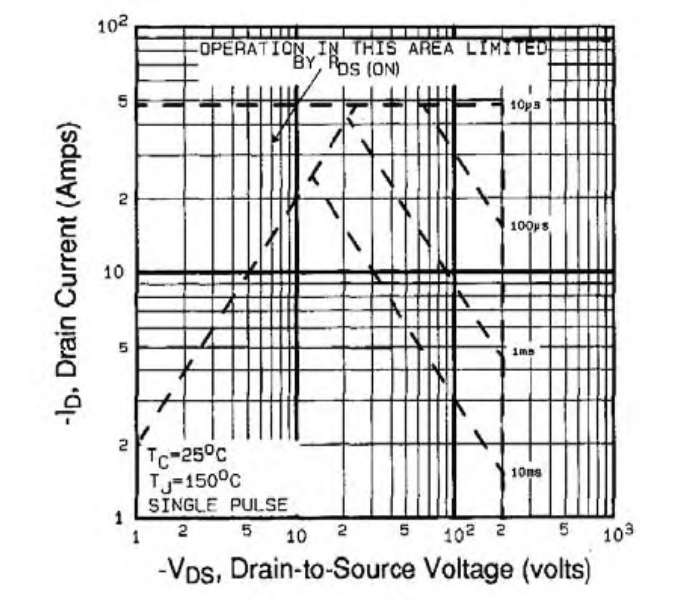
\includegraphics[width=0.8\textwidth]{SOA.png}
    }
    
    % Añadimos la fuente requerida por tu guía de TFG
    \vspace{2mm}
    {\raggedleft \textbf{Fuente:} Extraído de hoja de datos del IRFP9240PBF\cite{vishay_semiconductors_irfp9240pbfmosfet_nodate}. \par}
\end{figure}

En aplicaciones espaciales actuales, con los buses de voltajes mayores a los tradicionales, la potencia disipada vista en la \ref{eq:potencia_instantanea_lineal} puede superar con facilidad la capacidad térmica que soporta el encapsulado, llevando a un aumento de la temperatura en la unión ($T_\text{J}$) en pocos milisegundos. Esto podemos confirmarlo al analizar la curva del fabricante para la SOA del dispositivo (Figura \ref{fig:soa_mosfet}). En ella se observa que, para la comentada tensión de bus $(\vbus)$ de $100$ V, el componente puede soportar únicamente una corriente DC inferior a $0{,}4$ A sin que la integridad del dispositivo se vea comprometida. En la figura también se puede observar que el IRFP9240PBF es capaz de soportar corriente de $3$ A, pero únicamente al enfrentarse a transitorios de muy poca duración (pulsos de $1$ ms). 
Con todo lo expuesto, el diseño de LCL empleando P-MOS regulando de forma lineal la corriente se enfrenta a una problemática con difícil solución: para aumentar el tiempo de limitación y evitar la desconexión de la carga tras un transitorio se requiere el empleo de semiconductores de gran tamaño junto a sistemas de gestión térmica bien pasivos o bien activos, aumentando el valor de una variable crítica en los satélites como es la masa. 

\subsection{La transición al canal N (N-MOS) y materiales de banda prohibida ancha (WBG)}


La superioridad técnica de los dispositivos de canal N tiene su raíz física en la movilidad de los portadores de carga en el silicio. Mientras en un MOSFET de canal N el silicio está dopado de electrones que actúan de portadores, en un MOSFET de canal P los portadores mayoritarios son los huecos. 
La movilidad en los electrones $\mu_\text{e}$ a $300$ K en el silicio es de $1350 \, \text{cm}^2/\text{V}\cdot\text{s}$, mientras que la movilidad de los huecos ($\mu_p$) es prácticamente 3 veces menor, rondando los $480 \, \text{cm}^2/\text{V}\cdot\text{s}$ \cite{departamento_de_ingenieria_universidad_de_almeria_propiedades_nodate}. Estas diferencias de conductividad no son únicamente propias del silicio, sino que es común en otros semiconductores como el germanio o en aleaciones como el arseniuro de germanio (AsGe). 

Cualquier transistor en estado activo, es decir, durante el paso de corriente, tiene una cierta resistencia parásita que se opone a este paso. Esta resistencia es comunmente denominada $\rdson$ y, al igual que cualquier resistencia, sigue la ecuación expresada en \ref{eq:ResistenciaRDSON} donde $\rho$ representa la resistividad del material, $W$ el ancho del canal y $T$ la profundidad del mismo. 
\begin{equation}
	\rdson = \rho \frac{L}{W T}
\label{eq:ResistenciaRDSON}
\end{equation}

Considerando a ambos transistores (canal P y canal N) de las mismas dimensiones y sabiendo que la conductividad o movilidad ($\sigma$) es la inversa de la resistividad podemos llegar a la ecuación \ref{eq:conductividad} de donde se deduce que por tener los transistores de canal N una movilidad aproximadamente 3 veces mayor que la de los transistores de canal P, su resistencia de encendido será en torno a 3 veces menor. Esto a su vez supone que para que un P-MOS iguale la resistencia de un N-MOS requerirá aumentar su superficie de silicio por un factor de 3\cite{noauthor_p-channel-power-mosfets-and-their-impactful-applications_nodate}.

\begin{equation}
\rdson\propto \frac{1}{\sigma} = \frac{1}{q (n\mu_n + p\mu_p)}
\label{eq:conductividad}
\end{equation}

Sin embargo, el aumento del área de silicio no solo aumenta el coste del componente y su tamaño (volumen y masa) sino que incrementas las capacitancias parásitas y la carga de puerta, influyendo en el tiempo necesario para conmutar el dispositivo y, por tanto, disminuyendo el rendimiento durante la conmutación. 

Por tanto, pese a la simplicidad que supone el control de la puerta del P-MOS como se analizó en la sección anterior, la transición hacia buses de mayor potencia hace de las pérdidas por conducción un factor clave, especialmente teniendo en cuenta que en los LCL las pérdidas principales de los MOSFET son estas, pues solo conmuta durante la limitación tras fallo. Es por ello que con la aparición de las técnicas de bootstrap o los convertidores aislados necesarias para el control de la puerta en una configuración \textit{High-side} se ha producido una transición hacia los N-MOS.

\subsubsection{El papel de los materiales WBG (SiC y GaN)}

La transición al canal N, pese a ser el cambio principal y el más asentado, no se trata del único. El silicio presenta ciertas limitaciones como son su comportamiento respecto a las variaciones de temperatura y en conmutación. En los MOSFET, la movilidad de portadores disminuye debido al aumento de la temperatura de la unión ($T_\text{J}$) debido al fenómeno conocido como dispersión por vibraciones de la red (\textit{Lattice Scattering})\cite{ridley_quantum_2013}, incrementando la $\rdson$ y las pérdidas por conducción. 
Por otra parte, la banda prohibida del silicio es baja respecto a otro tipo de materiales. Esta magnitud representa las barreras de energía en semiconductores que deben superar los electrones para poder circular como corriente eléctrica \cite{noauthor_materiales_nodate}, obligando a diseños de capas más gruesas para soportar los 100 V y, por tanto, aumentando la resistencia interna del dispositivo.

Los materiales de banda prohibida ancha o WBG como el Carburo de Silicio (SiC) o el Nitruro de Galio (GaN) poseen una banda muy superior al Silicio, siendo en el SiC aproximadamente 3 veces superior, lo que se traduce en un campo eléctrico crítico mucho mayor. En la \ref{table:si_vs_sic} podemos observar algunas de las características principales que debemos observar en un semiconductor.

\begin{table}[H]
    \centering
    \fontsize{10}{12}\selectfont
    \ttabbox[\textwidth]
    {\caption{COMPARACIÓN DE PROPIEDADES FÍSICAS Y ELÉCTRICAS ENTRE SILICIO (SI) Y CARBURO DE SILICIO (SIC)}}
    {\begin{tabular}{|P{3.5cm}|P{4.5cm}|P{4.5cm}|}
        \hline
        \textbf{PARÁMETRO FÍSICO / ELÉCTRICO} & \textbf{SILICIO (SI)} & \textbf{CARBURO DE SILICIO (SIC)} \\
        \hline
        Banda prohibida ($E_g$) & $\sim 1{,}1$ eV & $\sim 3{,}2\text{--}3{,}3$ eV \\
        \hline
        Campo de ruptura máximo & $\sim 0{,}3$ MV/cm & $\sim 2{,}5\text{--}3$ MV/cm (unos $10\times$ mayor) \\
        \hline
        Resistencia encendido ($R_{on}$) & Alta, limitada por el campo & Muy baja, permite dispositivos de alta tensión pequeños \\
        \hline
        Conductividad térmica & $\sim 150\text{--}170$ W/(m·K) & $\sim 370\text{--}490$ W/(m·K) \\
        \hline
        Temperatura máxima de trabajo & Limitada ($< 150\text{--}175$ °C) & Hasta $\sim 200\text{--}250$ °C \\
        \hline
        Comportamiento en alta frecuencia ($Q_{\text{G}}$) & Adecuado, pero con pérdidas dinámicas mayores por mayor carga de puerta & Diseñado para alta frecuencia y eficiencia en PWM, carga de puerta menor \\
        \hline
        \multicolumn{3}{r}{\rule{0pt}{3ex}\textbf{Fuente:} Elaboración propia a partir de SA Materials \cite{noauthor_carburo_nodate} }
	\label{table:si_vs_sic}
    \end{tabular}}
\end{table}


Como vimos anteriormente en la ecuación \ref{eq:ResistenciaRDSON}, a mayor conductividad menor será la resistencia en conducción $\rdson$, por lo que la diferencia entre el Silicio y el Carburo de Silicio que podemos ver en la \ref{table:si_vs_sic} hace que podamos fabricar capas mucho más delgadas para la misma tensión, disminuyendo aun así la resistencia. Además, el rendimiento en alta frecuencia mejora enormemente debido a la carga de puerta reducida ($Q_{\text{G}}$), lo que provoca que los tiempos de apagado y encendido sean menores y, por tanto, las perdidas de conmutación menores, permitiendo llegar a frecuencias mayores. Por último, la conductividad térmica mayor del SiC permite que este evacúe el calor más rápido, permitiéndole trabajar a temperaturas mayores. 

La mejora en las condiciones del material es lo que permite trabajar de forma segura y cómoda a alta frecuencia y lo que nos ha permitido, como se verá en la siguiente sección, evolucionar desde la regulación lineal a la regulación conmutada durante la limitación en los LCL. 




\subsection{Estrategias de limitación de corriente: Operación Lineal vs. Conmutada}
La mejora en los materiales explicada en la sección anterior resultó en un cambio en el paradigma de la limitación. Mientras hasta el momento las pérdidas por conmutación en el Silicio eran demasiado altas y se recurría a limitación en la región lineal o zona activa, la evolución hacia el Carburo de Silicio y sus condiciones eléctricas y térmicas superiores permitieron el paso a limitadores en conmutación, haciendo uso de las topologías de convertidores de potencia desarrollados. 

\subsubsection{Limitadores en modo lineal}
Durante la operación lineal empleada en los LCLs tradicionales, el MOSFET actúa como una resistencia variable  controlada por la tensión y opera en su región activa. Siendo el objetivo limitar la corriente durante el fallo al valor de limitación ($I_\text{lim}$), el circuito de control se encarga de ajustar la tensión entre puerta y fuente ($V_\text{GS}$) manteniendo el canal parcialmente abierto y forzando una caida de tensión considerablemente alta entre el drenador y la fuente del dispositivo ($V_{DS}$). 

Este método se enfrenta a un problema principal que es la gestión térmica del semiconductor. El dispositivo absorbe la diferencia de voltaje entre el bus de entrada y la carga durante la limitación de corriente, por lo que la potencia instantánea definida en la ecuación \ref{eq:potencia_instantanea_lineal} se disparará. Teniendo en cuenta el paso a buses de 100 V, los límites marcados por el área segura de operaciones (SOA, mostrado en la figura \ref{fig:soa_mosfet}) son fácilmente excedibles, por lo que en esta zona la limitación será únicamente posible para pulsos muy cortos (microsegundos) para evitar la destrucción del semiconductor debido al estrés térmico. Debido a esto, los LCL lineales tradicionales requerirían de dispositivos de grandes dimensiones con disipadores de calor enormes para conseguir llegar a los \textit{trip-off times} de milisegundos empleados actualmente. 

\subsubsection{Limitadores en modo de conmutación}
Una vez vistas las limitaciones intrínsecas de la tecnología del Silicio en modo lineal y gracias a la llegada de los materiales WBG, la alternativa robusta para los LCL es el modo de conmutación. En este modo, el MOSFET deja de actuar como una resistencia variable y de limitar la corriente extra, sino que actúa conmutando a alta frecuencia mediante la modulación por ancho de pulso (en adelante PWM, por sus siglas Pulse Width Modulation) de la que se encarga un driver dedicado. Mediante esta estrategia y debido a la topología que se presentará en el siguiente capítulo, el LCL actúa como un convertidor reductor (\textit{Buck}) que, mediante la variación del ciclo de trabajo, regula la corriente media durante la limitación. 

La ventaja principal que podemos encontrar respecto a los limitadores lineales está en la eficiencia, ya que en vez de trabajar en la zona lineal (canal parcialmente abierto) como era el caso anterior, el transistor alterna entre el estado abierto ($I_\text{D} = 0$) y el de conducción ($V_\text{DS} \approx 0$), minimizando así las perdidas instantáneas de la ecuación \ref{eq:potencia_instantanea_lineal}. 
Las elevadas pérdidas que veíamos en el caso lineal que únicamente nos permitían pulsos de tiempo reducido son mucho más reducidas en este caso, siendo las pérdidas totales la suma de las de conducción debido a la corriente de limitación media a través de la resistencia parásita del MOSFET ($\rdson$) y las pérdidas de conmutación, siendo estas en dispositivos de Carburo de Silicio reducidas debido a la carga de puerta ($Q_\text{G}$). \cite{lopez_antuna_diseno_2024}. Es gracias a esto por lo que el semiconductor es capaz de resistir térmicamente la limitación durante un periodo de tiempo mayor, llegando a valores de hasta 20 ms para los LCL de clase 1 \cite{european_cooperation_for_space_standardization_ecss_ecss-e-st-20-20c_2016} impensables para los transistores en modo lineal si se pretende mantener el dispositivo en zona SOA.

Pese a ser una mejora en el cómputo global, el uso de una limitación conmutada introduce un rizado de corriente que puede ser perjudicial para la carga. Es por ello por lo que es recomendable el uso de una etapa de filtrado posterior al limitador que suavice la onda de corriente y suprimiendo así aquellos armónicos de alta frecuencia generados. La unión de ambas etapas permite una limitación precisa, de mayor tiempo y si el estrés térmico propio del modo lineal, mientras se mantiene la alimentación estable para la carga. 


\section{Tendencias en la protección de sistemas de potencia}
Una vez vista la evolución de los sistemas de protección hasta la actualidad es importante comentar que la mejora de estos sistemas no se centra únicamente en la mejora de los materiales de fabricación, sino que se extiende a un uso más óptimo de la energía \cite{adrian_garcia_hidalgo_diseno_nodate}. Es por eso que la tendencia actual en espacio es la transición hacia los controladores de potencia de estado sólido (en adelante, SSPC, por sus siglas en inglés Solid State Power Controllers), los cuales combinan protección con telemetría y diagnóstico \cite{noauthor_comprension_nodate}. 
\subsection{Digitalización y Reconfiguración}
\label{subsec:digit_reconfig}
El uso de lógica programable mediante el uso de microcontroladores o FPGA con certificación espacial permite que los limitadores de corriente pasen de ser estáticos a dispositivos inteligentes\cite{noauthor_comprension_nodate}. En los LCL tradicionales tanto la corriente de limitación como el tiempo de enclavamiento vienen determinados por redes de condensadores y resistencias, siendo una topología fija sin posibilidad de adaptación \cite{noauthor_proteccion_nodate}. Mediante el empleo de controladores los LCL pueden programarse para permitir distintos tipos de picos durante distintos momentos de operación, siendo más restrictivos durante la operación nominal y más permisivos en la conexión de carga. 
\subsection{Topologías de Próxima Generación}
A pesar de las mejoras obtenidas por el cambio hacia materiales WBG y transistores N-MOS, en aplicaciones con muy altas corrientes las pérdidas debido a la resistencia parásita provoca pérdidas significativas durante la no limitación \cite{noauthor_proteccion_nodate}. Es por ello que el futuro tiende hacia el uso en paralelo de un relé electromecánico junto a un SSCB, siendo el relé el encargado de conducir la corriente durante el estado estacionario debido a su baja resistencia y siendo el interruptor de estado sólido el encargado de gestionar los transitorios debido a la velocidad de respuesta y la no aparición de arcos eléctricos \cite{adrian_garcia_hidalgo_diseno_nodate}. 

\subsection{Discriminación de Fallos}
Mediante el uso de controladores lógicos como los microcontroladores o FPGA mencionados en la sección \ref{subsec:digit_reconfig} es posible implementar sistemas con algoritmos basados en curvas de energía. Estos, a diferencia de los LCL convencionales, no actúan en un umbral fijo, sino que, mediante la integración digital de la corriente en el tiempo, permite el paso de la energía necesaria para estabilizar la carga sin necesidad de desconectarla. De esta manera únicamente desconecta de forma instantánea la carga en casos extremos de corriente (cortocircuitos) donde la carga podría sufrir o incluso destruirse. De esta manera la potencia en el satélite se mantiene constante, aumentando la disponibilidad del mismo y la robustez frente a paradas\cite{noauthor_comprension_nodate}.

\section{Síntesis de la situación}

Con el objetivo de concluir el análisis realizado en el capítulo, en esta última sección se sintetizan los pilares que justifican la transición hacia nuevos materiales, topologías y métodos de limitación. El escenario aeroespacial actual, con el aumento del voltaje de los buses, presenta tres conclusiones principales:

\begin{enumerate}
    \item \textbf{Idoneidad de los materiales WBG y canal N:} La superioridad de los MOSFET de canal N de Carburo de Silicio (SiC) supone el núcleo central de la evolución tecnológica de la solución. La alta movilidad obtenida por el paso al canal N se ve incrementada por la mayor movilidad intrínseca del SiC, lo que junto a la menor carga de puerta ($Q_\text{g}$) permiten una mayor frecuencia de conmutación manteniendo pérdidas mínimas. La mejora en las propiedades es la que nos permite desplazarnos hacia frecuencias de conmutación mayores sin afectar negativamente a la eficiencia del sistema. 
    \item \textbf{Inviabilidad térmica del modo lineal:} El aumento de la tensión nominal en los buses de satélites hasta los 100 V hace inviable el uso de limitadores clásicos que actúen en la región lineal o activa. Como se ha visto en anteriores secciones, el semiconductor debe disipar la potencia instantánea de la ecuación \ref{eq:potencia_instantanea_lineal} durante la sobrecorriente, sobrepasando las limitaciones de los encapsulados estándar y, salvo en pulsos extremadamente cortos, saliendo del Área de Operación Segura (SOA). Esta restricción térmica lleva al diseño de sistemas en los que el semiconductor no esté expuesto a un estrés tan alto durante la limitación.
    \item \textbf{Regulación por conmutación (PWM):} El estrés térmico y las grandes pérdidas de los sistemas lineales nos llevan a la transición hacia un sistema basado en modulación por ancho de pulso. Además de reducir el estrés térmico por ser las pérdidas principalmente la suma de las de conmutación y las producidas por la resistencia parásita del MOSFET, esta regulación reduce la masa del sistema al poder reducir el volumen de los sistemas de disipación y optimiza, por tanto, un parámetro importante en satélites. 
\end{enumerate}

En los siguientes capítulos se partirá de lo expuesto hasta el momento para desarrollar una solución viable que mejore las prestaciones de los sistemas lineales tradicionales. La propuesta se basará en el uso de un limitador de corriente de enclavamiento conmutado para proporcionar una protección eficiente, a altas frecuencias de conmutación y estable térmicamente.


\chapter{Diseño teórico del LCL conmutado}

Este capítulo presenta el núcleo teórico del diseño del limitador de corriente de enclavamiento propuesto, basado en la topología propuesta por López et al. \cite{lopez_antuna_diseno_2024}. Tras el análisis de los componentes y materiales óptimos para esta aplicación en el capítulo anterior, en esta sección se muestra el funcionamiento y los subcircuitos que conforman esta arquitectura conmutada empleando el MOSFET de canal N. 

El objetivo principal es establecer las bases y ecuaciones que rigen el comportamiento del convertidor. Durante este primer análisis, se emplearán en su mayor parte componentes ideales para explicar la lógica de control, de temporización y el sensado de corriente, permitiendo aislar estos análisis de los componentes parásitos o de los tiempos de conmutación que aparecen al considerar componentes no ideales. De esta manera, se estudiará el dimensionado de la inductancia y el lazo de control, estableciendo una base teórica antes del estudio de pérdidas y la selección de componentes. 

Con el objetivo de no repetir los cálculos tanto con valores genéricos como con los valores reales, las cuentas se realizarán directamente con los valores obtenidos de las hojas de datos de los componentes. La selección de estos componentes serán justificados en el siguiente capítulo. 
\section{Especificaciones y requerimientos de diseño}
\label{secc: Especificaciones y requerimientos de diseño}
Los valores seleccionados en un Limitador de Corriente de Enclavamiento (LCL) no sono arbitrarios, sino que están seleccionados teniendo en cuenta tanto el bus de potencia principal como la carga a proteger. Durante el diseño de este tipo de dispositivos, los parámetros principales a tener en cuenta son la tensión del bus ($\vbus$), la corriente a la que limitará el dispositivo ($I_\text{lim}$) y el tiempo de disparo o \textit{trip-off time} ($t_\text{trip}$). 
\subsection{Parámetros fundamentales y clases de LCL}

En el ámbito aeroespacial, sector en el que se sigue la normativa \textbf{ECSS-E-ST-20C} \cite{european_space_agency_ecss-e-st-20c_2022}, están establecidas una serie de clases predefinidas para los LCL de 28 V. El uso de estas clases donde los parámetros principales mencionados anteriormente son establecidos aseguran que todas las partes encargadas de la fabricación de la carga, el sistema de potencia... compartan unas reglas comunes para la protección. En la Tabla \ref{table:EstandarLCL} se han recopilado los valores típicos en función de la clase. 


\begin{table}[H]
   \centering
    
   \fontsize{10}{12}\selectfont
   \ttabbox[\textwidth]
   {\caption{CLASES ESTÁNDAR DE LCL PARA BUS DE 28 V}}
  {\begin{tabular}{|P{2cm}|P{3,5cm}|P{3.5cm}|P{3.5cm}|}
        \hline
        \textbf{CLASE} & \textbf{CORRIENTE DE CLASE (A)} & \textbf{RANGO DE CORRIENTE DE LIMITACIÓN (A)}& \textbf{RANGO DE TIEMPO DE LIMITACIÓN (ms)} \\
        \hline
        1 & 1 & $1{,}1\text{--}1{,}4$ & $10\text{--}20$ \\
        \hline
        2 & 2 & $2{,}2\text{--}2{,}8$ & $10\text{--}20$ \\
        \hline
        3 & 3 & $3{,}3\text{--}4{,}2$ & $6\text{--}12$ \\
        \hline
        4 & 4 & $4{,}4\text{--}5{,}6$ & $6\text{--}12$ \\
        \hline
        5 & 5 & $5{,}5\text{--}7$ & $4\text{--}8$ \\
        \hline
        6 & 6 & $6{,}6\text{--}8{,}4$ & $2\text{--}4$ \\
        \hline
        8 & 8 & $8{,}8\text{--}11{,}2$ & $2\text{--}4$ \\
        \hline
        10 & 10 & $11\text{--}14$ & $1{,}5\text{--}3$ \\
        \hline
        \multicolumn{4}{r}{\rule{0pt}{3ex}\textbf{Fuente:} Elaboración propia a partir de la ECSS-E-ST-20-20CSA \cite{european_cooperation_for_space_standardization_ecss_ecss-e-st-20-20c_2016} }
    \label{table:EstandarLCL}
\end{tabular}}
\end{table}



\subsection{Personalización del diseño para bus de 100 V}

Una característica singular de este trabajo es el uso de un bus de 100 V, como se ha visto en secciones anteriores. Los buses de 100 V, a diferencia de los de 28 V o los de 50 V, no son todavía ampliamente utilizados, lo que provoca que no contemos con una tabla de clases estandarizada para este voltaje. Esto nos otorga libertad a la hora de elegir las características principales de nuestro sistema y a su vez nos obliga a justificar aquellas decisiones que tomemos, tanto en cuanto a voltaje, corriente y tiempo como en cuanto a componentes. 

Para el LCL diseñado se han seleccionado las siguientes especificaciones:

\begin{itemize}
    \item \textbf{Tensión de bus nominal ($\vbus$):} 100 V.
    \item \textbf{Corriente de limitación ($I_\text{lim}$):} Para la carga y aplicación buscada para el prototipo, se ha escogido una corriente de limitación de 3,7 A.
    \item \textbf{Tiempo de trip-off ($t_\text{trip}$):} Debido a operar con un bus de mayor voltaje, la potencia disipada por el MOSFET durante esta etapa de limitación aumenta a prácticamente 4 veces el valor disipado en los buses de 28 V. Es por ello por lo que se ha decidido seleccionar el tiempo de \textit{trip-off} más restrictivo de las clases de 28 V siendo este 1,5 ms.
\end{itemize}

\subsection{Enfoque del prototipado}

Antes de entrar en el diseño y selección de componentes para el prototipo, es necesario subrayar que el dispositivo diseñado cumple con objetivos de validación funcional en un entorno de laboratorio. Es por ello por lo que las estríctas reglas y estándares aeroespaciales (tanto a nivel de componentes como a nivel diseño) no se han seguido en todo momento, dejando el refinado de estos puntos para una iteración posterior del prototipo. No obstante, a pesar de esta flexibilidad necesaria en fase de investigación, todos los criterios de selección de la topología (uso de MOSFET de canal N, gestión del rizado y protecciones) se han orientado para ser compatibles con el sector aeroespacial y tener una escalabilidad sencilla. 

Además, otro objetivo es permitir la experimentación con distintos valores de limitación de corriente y diferentes tiempos mediante el cambio de un número mínimo de componentes como se verá en secciones posteriores. 
\section{Arquitectura del limitador basado en N-MOS}
\label{section:Arquitectura}
En el capítulo anterior se ha justificado la idoneidad del uso de dispositivos de canal N frente a los de canal P debido a las diferencias en términos de resitencias parásitas y a la influencia de este factor en la eficiencia y gestión térmica del dispositivo. En esta sección se partirá del uso de un N-MOS para mostrar la estructura de convertidor reductor o \textit{Buck} que emplearemos para la operación de este dispositivo en topología \textit{high-side}, centrándonos tanto en el diseño de la parte de potencia como en la parte de control formada por los bloques de temporización, sensado e histéresis.

\subsection{Topología conmutada y configuración de potencia}

La etapa de potencia del LCL se diseña empleando una topología de convertidor \textit{Buck}, lo que implica que el N-MOS está situado en el lado de alta tensión para actuar como elemento de corte en serie con la carga.

A diferencia de los convertidores reductores habituales, en el diseño de este limitador se prescinde del condensador de salida. Esto se debe a que el objetivo del circuito es permitir que sea únicamente la bobina la encargada de control de forma dinámica la corriente. El condensador de salida, al reducir el rizado, dificulta la detección instantánea de variaciones provocadas por la carga y es por ello por lo que se evita el uso del mismo. 

El circuito, basado en la topología propuesta por López et al. \cite{lopez_antuna_diseno_2024}, se puede observar en la Figura \ref{fig:convertidor_histeresis}: 

\begin{figure}[H]
    \centering
    \fontsize{10}{12}\selectfont 
    
    \ffigbox[\FBwidth]
    {
        \caption{Esquema del convertidor y sistema de control implementado}
        \label{fig:convertidor_histeresis}
    }
    {
        \begin{tikzpicture}[transform shape]
            % Paths, nodes and wires:
            \draw (11.373, 8.453) |- (11.333, 7.111);
            \draw (16.368, 4.614) -- (15.257, 4.614);
            \node[shape=rectangle, fill={rgb,255:red,255;green,255;blue,255}, draw={rgb,255:red,0;green,0;blue,0}, line width=1pt, minimum width=1.606cm, minimum height=1.08cm](N1) at (11.169, 6.669){} node[anchor=center] at (N1.text){$Driver$};
            \draw (19.111, 7.644) |- (19.111, 8.033);
            \draw (7.389, 8.928) to[american voltage source, l_={$Vbus$}, name=Vbus] (7.389, 8.178);
            \draw (9.056, 8.705) to[capacitor, /tikz/circuitikz/bipoles/length=0.980cm, l={$Cbus$}, label distance=-0.07cm] (9.056, 8.372);
            \node[nigfete, rotate=90](N2) at (11.103, 9.433){} node[anchor=south] at ([yshift=-0.09cm]N2.text){$NMOS$};
            \draw (12.75, 8.683) to[empty Schottky diode, /tikz/circuitikz/bipoles/length=0.840cm] (12.75, 9.183);
            \draw (15.125, 9.433) to[american inductor, i=$i_\textbf{L}(t)$, current/distance=1] (17.25, 9.433);
            \draw (13.25, 9.433) to[american resistor, l_={$R shunt$}] (14.75, 9.433);
            \draw (17.556, 7.705) to[american resistor, l={$Carga$}] (17.556, 9.205);
            \draw (12.75, 9.433) -- (12.75, 9.183);
            \draw (12.29, 9.433) -- (13.25, 9.433);
            \draw (15.125, 9.433) -- (14.75, 9.433);
            \draw (16.875, 9.433) -- (17.25, 9.433) -| (17.556, 9.205);
            \draw (9.056, 8.933) -| (9.056, 9.433) -- (9.556, 9.433);
            \node[ground] at (9.056, 7.705){};
            \node[ground] at (12.75, 7.683){};
            \node[ground] at (17.556, 7.705){};
            \node[ground] at (7.389, 7.678){};
            \draw (7.389, 8.178) -| (7.389, 7.678);
            \draw (9.056, 9.433) -| (7.389, 9.428);
            \draw (7.389, 9.428) -| (7.389, 8.928);
            \draw (9.056, 8.372) -| (9.056, 7.372);
            \draw (12.75, 8.683) -| (12.75, 7.683);
            \draw (19.111, 9.034) to[american voltage source, l={$Vcc$}] (19.111, 8.283);
            \draw (19.111, 7.783) -- (19.111, 8.283);
			\node[shape=rectangle, minimum width=1.801cm, minimum height=1.076cm] at (20.111, 7.556){} node[anchor=north west, align=left, text width=1.427cm, inner sep=5.8pt] at (19.193, 8.111){Masa Control};
			\node[ocirc] at (19.111, 7.783){};
			\draw (13.183, 10.193) -| (12.75, 9.433);
			\node[ocirc] at (13.235, 10.193){};
			\node[shape=rectangle, minimum width=2.737cm, minimum height=0.455cm] at (14.569, 10.193){} node[anchor=center, align=center, text width=2.561cm, inner sep=3pt] at (14.569, 10.193){Masa Control};
			\draw (19.111, 9.534) -| (19.111, 9.034);
			\node[ocirc, xscale=-1, yscale=-1](N3) at (19.111, 9.534){} node[anchor=north] at ([yshift=0.52cm]N3.text){$Vcc$};
			\node[sground] at (19.111, 7.644){};
			\node[ieeestd and port, rotate=90, xscale=0.72, yscale=0.72] at (11.333, 5.333){};
			\draw (17.205, 3.486) |- (17.705, 3.486);
			\node[ocirc, rotate=90] at (17.205, 3.486){};
			\node[shape=rectangle, minimum width=1.525cm, minimum height=0.665cm] at (16.425, 3.486){} node[anchor=north west, align=left, text width=1.137cm, inner sep=6pt] at (15.644, 3.836){Vsense};
			\draw (15, 8.211) -| (15, 8.711);
			\draw (15, 8.156) -- (15, 8.656);
			\node[ocirc, xscale=-1, yscale=-1] at (15, 8.156){};
			\node[shape=rectangle, minimum width=1.165cm, minimum height=0.865cm] at (15.044, 7.883){} node[anchor=center, align=center, text width=0.988cm, inner sep=3pt] at (15.044, 7.883){Vmeas};
			\node[shape=rectangle, minimum width=1.703cm, minimum height=0.865cm] at (14.833, 2.392){} node[anchor=center, align=center, text width=1.526cm, inner sep=3pt] at (14.833, 2.392){Vmeas};
			\node[shape=rectangle, fill={rgb,255:red,255;green,255;blue,255}, draw={rgb,255:red,0;green,0;blue,0}, line width=1pt, minimum width=3.076cm, minimum height=1.076cm] at (17.979, 4.392){} node[anchor=center, align=center, text width=2.688cm, inner sep=6pt] at (17.979, 4.392){Control por Histéresis\\};
			\node[shape=rectangle, fill={rgb,255:red,255;green,255;blue,255}, draw={rgb,255:red,0;green,0;blue,0}, line width=1pt, minimum width=3.131cm, minimum height=1.076cm] at (13.563, 4.392){} node[anchor=center, align=center, text width=2.743cm, inner sep=6pt] at (13.563, 4.392){Biestable\\};
			\node[shape=rectangle, minimum width=1.187cm, minimum height=0.374cm] at (15.757, 4.965){} node[anchor=north, align=center, text width=0.799cm, inner sep=6pt] at (15.757, 5.17){Set};
			\node[shape=rectangle, minimum width=1.187cm, minimum height=0.352cm] at (15.757, 4.343){} node[anchor=north, align=center, text width=0.799cm, inner sep=6pt] at (15.757, 4.536){Reset};
			\draw[-latex] (16.313, 4.614) -- (15.146, 4.614);
			\draw[-latex] (16.368, 3.993) -- (15.146, 3.993);
			\draw (11.535, 4.554) -- (11.535, 4.392) -- (11.979, 4.392);
			\node[shape=rectangle, minimum width=1.187cm, minimum height=0.52cm] at (11.651, 4.233){} node[anchor=north, align=center, text width=0.799cm, inner sep=6pt] at (11.651, 4.51){Q};
			\draw[-latex] (18.007, 2.948) -| (17.979, 3.836);
			\node[shape=rectangle, fill={rgb,255:red,255;green,255;blue,255}, draw={rgb,255:red,0;green,0;blue,0}, line width=1pt, minimum width=3.131cm, minimum height=1.076cm] at (7.874, 4.399){} node[anchor=center, align=center, text width=2.743cm, inner sep=6pt] at (7.874, 4.399){Temporizador\\};
			\draw (10.702, 4.392) -| (11.132, 4.554);
			\node[shape=rectangle, minimum width=1.742cm, minimum height=0.512cm] at (10.243, 4.281){} node[anchor=north, align=center, text width=1.354cm, inner sep=6pt] at (10.243, 4.554){Shutdown};
			\draw (10.702, 4.392) -| (9.457, 4.399);
			\node[shape=rectangle, minimum width=1.631cm, minimum height=0.665cm] at (8.096, 3.083){} node[anchor=north west, align=left, text width=1.243cm, inner sep=6pt] at (7.263, 3.433){Vsense};
			\draw (15.702, 2.392) |- (16.202, 2.392);
			\node[ocirc, rotate=90] at (15.702, 2.392){};
			\draw (8.096, 3.383) -| (8.096, 3.883);
			\node[ocirc, xscale=-1, yscale=-1] at (8.096, 3.383){};
			\draw (15, 8.656) -| (15, 9.433);
			\node[shape=rectangle, minimum width=1.165cm, minimum height=0.514cm] at (16.289, 9.202){} node[anchor=center, align=center, text width=0.988cm, inner sep=3pt] at (16.289, 9.202){L};
			\node[shape=rectangle, minimum width=1.165cm, minimum height=0.865cm] at (12.956, 8.539){} node[anchor=center, align=center, text width=0.988cm, inner sep=3pt] at (12.956, 8.539){D};
			\draw (6.651, 5.455) -| (6.651, 4.955);
			\node[ocirc, xscale=-1, yscale=-1](N4) at (6.651, 5.455){} node[anchor=north] at ([yshift=0.52cm]N4.text){$Vcc$};
			\draw (13.563, 5.448) -| (13.563, 4.947);
			\node[ocirc, xscale=-1, yscale=-1](N5) at (13.563, 5.448){} node[anchor=north] at ([yshift=0.52cm]N5.text){$Vcc$};
			\draw (19.313, 3.448) -| (19.313, 2.948);
			\node[ocirc, xscale=-1, yscale=-1](N6) at (19.313, 3.448){} node[anchor=west] at ([xshift=0.09cm]N6.north east){$Vcc$};
			\node[sground] at (19.318, 1.899){};
			\node[sground] at (13.563, 3.836){};
			\node[sground] at (6.651, 3.844){};
			\node[sground] at (18.535, 3.836){};
			\draw (18.535, 5.448) -| (18.535, 4.948);
			\node[ocirc, xscale=-1, yscale=-1](N7) at (18.535, 5.448){} node[anchor=west] at ([xshift=0.09cm]N7.north east){$Vcc$};
			\draw (17.705, 3.486) -| (17.986, 3.503);
			\draw (10.54, 7.733) -| (10.54, 7.233);
			\node[ocirc, xscale=-1, yscale=-1](N8) at (10.54, 7.733){} node[anchor=north] at ([yshift=0.52cm]N8.text){$Vcc$};
			\node[sground] at (10.54, 6.122){};
			\node[shape=rectangle, fill={rgb,255:red,255;green,255;blue,255}, draw={rgb,255:red,0;green,0;blue,0}, line width=1pt, minimum width=3.465cm, minimum height=1.076cm] at (17.952, 2.392){} node[anchor=center, align=center, text width=3.077cm, inner sep=6pt] at (17.952, 2.392){Sensor Corriente\\(Ganancia K)};
			\draw (12.29, 9.433) -- (11.873, 9.433);
			\draw (9.556, 9.433) -- (10.333, 9.433);
			\draw (9.056, 8.933) |- (9.056, 8.705);
            % ... (resto del tikz EXACTAMENTE igual)
        \end{tikzpicture}
    }
    
    \vspace{2mm}
    {\raggedleft \textbf{Fuente:} Elaboración propia basada en la topología de López et al. \cite{lopez_antuna_diseno_2024}. \par}
\end{figure}

Uno de los elementos críticos al emplear un N-MOS en arquitectura \textit{high-side} es asegurar un correcto ciclo de trabajo durante la no limitación. En condiciones nominales, el transistor debe conducir de forma constante, es decir, tener un ciclo de trabajo (D) igual a 1 para así asegurar el suministro en la carga de los 100 V de la entrada. 

Por tratarse de un N-MOS en \textit{high-side} es necesario para que el dispositivo conduzca que haya en la puerta del mismo en torno a 15 voltios más que el voltaje del bus, lo que imposibilita el uso de técnicas tradicionales como el uso de un condensador \textit{bootstrap} ya que estos requieren de la conmutación para recargar el condensador. Empleando un ciclo de trabajo constante de 1 sería inevitable la descarga del condensador y, por tanto, el cierre del canal del MOSFET, lo que llevaría a la desconexión de la carga. 

Es por ello por lo que se ha decidido emplear una fuente de alimentación flotante la cual añadirá 15 voltios al voltaje que podemos ver en la Figura \ref{fig:convertidor_histeresis} como masa flotante. De esta manera, nos aseguramos tener siempre una señal capaz de polarizar la puerta del MOSFET al ser el voltaje total de esta señal dependiente del voltaje en la fuente del transistor y por tanto $V_\text{GS}$ constante y suficiente para asegurar el trabajo en saturación. 

Otro de los componentes principales para asegurar una correcta conmutación es el diodo de libre circulación. Durante el tiempo de apagado $\Toff$ del transistor, la energía almacenada en el inductor debe descargarse antes del próximo periodo de conmutación. Al estar abierto el circuito por el transistor, el diodo permite cerrar el circuito y que así la corriente siga circulando hacia la carga. La presencia de este diodo evita que la corriente icircule hacia el transistor y provoque en él una sobrecorriente que pueda destruirlo. Para aumentar la eficiencia de la conmutación, se emplea un diodo Schottky cuya carga de recuperación ($Q_\text{rr}$) es nula.

El condensador $C_\text{bus}$ por su parte actúa como condensador de filtrado para el voltaje del bus de entrada. Cuenta con varias funcióes como son el almacenar energía actuando como reserva para estabilizar el voltaje, suministrar los picos de corriente de alta frecuencia durante la conmutación, abosrber la inductancia de cables externos y actuar como filtro. Debido a la naturaleza de las funciones expuestas, el condensador requiere de una alta capacidad para actuar como reserva a la vez que es necesario que actúe a alta velocidad durante la conmutación. Es por ello que, pese a modelarlo en la Figura \ref{fig:convertidor_histeresis} como un solo condensador, emplearemos uno de baja capacidad junto a uno de alta capacidad en paralelo para cumplir ambas funciones. 

\subsection{Sensado y acondicionamiento de señal}

Para que el driver sepa cuando hacer conmutar al MOSFET, es necesario contar con una manera de medir la corriente que circula hacia la carga. Debido a la dificultad para la medida de la corriente en sí, se emplea una resistencia de medida ($R_\text{shunt}$) de baja inductancia y se toma el valor del voltaje antes (masa control) y después de la misma ($V_\text{meas}$). Empleando una resistencia con una baja tolerancia y siendo la caida de voltaje proporcional a la corriente por ella, se sabe con exactitud la corriente que fluye hacia la carga. 
\begin{figure}[H]
    \centering
    \fontsize{10}{12}\selectfont 
    
    \ffigbox[\FBwidth]
    {
        \caption{Bloque de sensado y acondicionamiento de señal}
        \label{fig:sensadoCorriente}
    }
    {
   \begin{tikzpicture}[transform shape]
	% Paths, nodes and wires:
	\node[op amp, xscale=0.52, yscale=0.52] at (6.25, 7.25){};
	\node[op amp, xscale=0.52, yscale=0.52] at (9.619, 6.995){};
	\draw (5.25, 8.5) to[american resistor, l={$R2$}] (7, 8.5);
	\draw (8.75, 8.25) to[american resistor, l={$R4$}] (10.5, 8.25);
	\draw (3, 8.5) to[american resistor, l={$R1$}] (4.75, 8.5);
	\draw (6.869, 7.25) to[american resistor, l={$R3$}] (8.619, 7.25);
	\draw (8.619, 7.25) -- (9, 7.25);
	\draw (8.75, 8.25) -- (8.75, 7.25);
	\draw (10.5, 8.25) |- (10.238, 6.995);
	\draw (7, 8.5) -- (7, 7.25);
	\draw (5.25, 8.5) -| (5.25, 7.5) -| (5.631, 7.505);
	\draw (4.75, 7) -| (5.631, 6.995);
	\node[shape=rectangle, minimum width=1.703cm, minimum height=0.865cm] at (4, 7){} node[anchor=center, align=center, text width=1.526cm, inner sep=3pt] at (4, 7){Vmeas};
	\draw (5.5, 9.5) to[capacitor, /tikz/circuitikz/bipoles/length=0.700cm, l={$C1$}] (6.75, 9.5);
	\draw (6.75, 9.5) -| (7, 8.5);
	\draw (5.5, 9.5) -- (5.25, 9.5) -- (5.25, 8.5);
	\draw (4.75, 8.5) -- (5.25, 8.5);
	\draw (9, 9.25) to[capacitor, /tikz/circuitikz/bipoles/length=0.700cm, l={$C2$}] (10.25, 9.25);
	\draw (10.25, 9.25) -| (10.5, 8.25);
	\draw (9, 9.25) -- (8.75, 9.25) -- (8.75, 8.25);
	\node[shape=rectangle, minimum width=1.525cm, minimum height=0.665cm] at (11.5, 7){} node[anchor=north west, align=left, text width=1.137cm, inner sep=6pt] at (10.72, 7.35){Vsense};
	\node[sground] at (2.75, 8.25){};
	\draw (2.75, 8.25) -| (2.75, 8.5) -- (3, 8.5);
	\node[sground] at (8.75, 6.5){};
	\draw (8.75, 6.5) -| (8.75, 6.75) -- (9, 6.75);
	\node[shape=rectangle, minimum width=3.715cm, minimum height=1.215cm] at (7.75, 5.75){} node[anchor=north west, align=left, text width=3.341cm, inner sep=5.8pt] at (5.875, 6.375){Masa Control};
	\node[shape=rectangle, minimum width=3.59cm, minimum height=1.367cm] at (1.813, 7.451){} node[anchor=north west, align=left, text width=3.216cm, inner sep=5.8pt] at (0, 8.153){Masa Control};
	\draw (10.75, 7) -- (10.5, 7);
\end{tikzpicture}
    }
    
    \vspace{2mm}
    {\raggedleft \textbf{Fuente:} Elaboración propia basada en la topología de López et al. \cite{lopez_antuna_diseno_2024}. \par}
\end{figure}
Debido a los valores de corriente y al bajo valor de la resistencia de medida, la señal es de bajo valor. Es por ello por lo que, en un sistema con conmutación y por tanto rizado de corriente, esta caida de tensión podría pasar desapercibida. 

Para solucionar esta problemática se emplean dos amplificadores operacionales alimentados entre la masa de control y la alimentación flotante en cascada con una ganancia de entorno a -25 V/V. Esta ganancia es inversora ya que la masa de control se encuentra antes que el punto de medida.
Esto como vemos en la ecuación \ref{eq:gananciaSensado} transforma una caída de voltaje de en torno a los 100 mV en un voltaje con el que podemos trabajar más cómodamente de en torno a los 2,5 V. En una aplicación crítica donde un pequeño incremento de corriente puede implicar la pérdida de la carga, es preciso poder distinguir claramente si la corriente que fluye es una sobrecorriente o no y, alejando ambos valores entre sí, se simplifica esta tarea. 

\begin{equation}
    G = \frac{V_{\text{sense}}}{V_{\text{meas}}} = \left( 1 + \frac{R_2}{R_1} \right) \cdot \left( - \frac{R_4}{R_3}\right) \approx -25
\label{eq:gananciaSensado}
\end{equation}

Por otro lado, los amplificadores en cascada implementan condensadores para actuar como filtros activos de ruidos de alta frecuencia debido a la conmutación. Este filtrado permite evitar que la limitación salte debido a un falso positivo por el rizado de la conmutación. 
La señal amplificada y filtrada es equivalente a la corriente que fluye hacia la carga y será la empleada en la etapa de temporización y en la etapa de histéresis para determinar tanto si se debe pasar a la limitación conmutada como si se ha superado el \textit{trip-off time}.



\subsection{Lógica de control y enclavamiento}

El funcionamiento durante una sobrecorriente viene determinado por el bloque temporizador y el bloque de histéresis de la Figura \ref{fig:histeresistemporizacion}. 
La caída de tensión acondicionada medida en la resistencia ($V_\text{sense}$) llega a ambos bloques y se compara con referencias flotantes, siendo un incremento de voltaje respecto al del bus. 
\begin{figure}[H]
    \centering
    \fontsize{10}{12}\selectfont 
    
    \ffigbox[\FBwidth]
    {
        \caption{Bloque de temporización e histéresis}
        \label{fig:histeresistemporizacion}
    }
    {
   \begin{tikzpicture}[transform shape]
	% Paths, nodes and wires:
	\node[shape=rectangle, fill={rgb,255:red,255;green,255;blue,255}, draw={rgb,255:red,0;green,0;blue,0}, line width=1pt, minimum width=1.606cm, minimum height=1.08cm](N1) at (4.505, 9.202){} node[anchor=center] at (N1.text){$Driver$};
	\node[ieeestd and port, xscale=-0.72, yscale=-0.72] at (6.104, 9.202){};
	\node[op amp, xscale=-0.52, yscale=0.52] at (11.82, 8.2){};
	\node[op amp, xscale=-0.52, yscale=0.52] at (11.82, 6.4){};
	\draw (11.401, 8.2) -- (10.92, 8.2);
	\draw (10.92, 6.4) -- (11.401, 6.4);
	\draw (12.438, 7.945) -| (12.72, 6.7) |- (12.438, 6.655);
	\draw (12.438, 6.145) -| (13.35, 6.145);
	\draw (12.438, 8.455) -| (13.35, 8.454);
	\draw (12.72, 7.3) -- (13.32, 7.3);
	\node[shape=rectangle, minimum width=1.525cm, minimum height=0.665cm] at (13.9, 7.3){} node[anchor=north west, align=left, text width=1.137cm, inner sep=6pt] at (13.12, 7.65){Vsense};
	\node[shape=rectangle, minimum width=1.525cm, minimum height=0.665cm] at (13.9, 8.45){} node[anchor=north west, align=left, text width=1.137cm, inner sep=6pt] at (13.12, 8.8){Vsuperior};
	\node[shape=rectangle, minimum width=1.525cm, minimum height=0.665cm] at (13.939, 6.15){} node[anchor=north west, align=left, text width=1.137cm, inner sep=6pt] at (13.159, 6.5){Vinferior};
	\draw (6.945, 8.22) -- (7.302, 8.22) -| (9.363, 8.27);
	\node[shape=rectangle, fill={rgb,255:red,255;green,255;blue,255}, draw={rgb,255:red,0;green,0;blue,0}, line width=1pt, minimum width=1.665cm, minimum height=2.565cm] at (10.07, 7.35){};
	\node[shape=rectangle, minimum width=0.665cm, minimum height=0.665cm] at (9.47, 8.25){} node[anchor=north west, align=left, text width=0.277cm, inner sep=6pt] at (9.12, 8.6){Q};
	\node[shape=rectangle, minimum width=0.665cm, minimum height=0.665cm] at (10.67, 8.2){} node[anchor=north west, align=left, text width=0.277cm, inner sep=6pt] at (10.32, 8.55){R};
	\node[shape=rectangle, minimum width=0.665cm, minimum height=0.665cm] at (10.72, 6.45){} node[anchor=north west, align=left, text width=0.277cm, inner sep=6pt] at (10.37, 6.8){S};
	\node[op amp, xscale=-0.52, yscale=0.52] at (8.7, 10.995){};
	\node[op amp, xscale=-0.52, yscale=0.52] at (14.3, 11.25){};
	\draw (11.2, 11.25) to[empty diode, /tikz/circuitikz/bipoles/length=0.700cm] (11.9, 11.25);
	\node[shape=rectangle, minimum width=1.525cm, minimum height=0.665cm] at (15.58, 11){} node[anchor=north west, align=left, text width=1.137cm, inner sep=6pt] at (14.8, 11.35){Vsense};
	\node[shape=rectangle, minimum width=1.525cm, minimum height=0.665cm] at (15.52, 11.5){} node[anchor=north west, align=left, text width=1.137cm, inner sep=6pt] at (14.739, 11.85){VTimON};
	\draw (13.6, 11.25) to[american resistor] (11.719, 11.25);
	\draw (13, 12.05) to[empty diode, /tikz/circuitikz/bipoles/length=0.700cm] (11.9, 12.05);
	\draw (13, 12.05) -| (13.5, 11.25);
	\draw (11.981, 12.05) -- (11.281, 12.05) -| (11.2, 11.25);
	\draw (13.6, 11.25) -- (13.9, 11.25);
	\draw (11.2, 11.25) -- (10.2, 11.25);
	\node[shape=rectangle, minimum width=1.525cm, minimum height=0.665cm] at (9.88, 10.75){} node[anchor=north west, align=left, text width=1.137cm, inner sep=6pt] at (9.1, 11.1){VTimON};
	\draw (10.2, 11.25) -| (9.319, 11.245);
	\draw (11.2, 11) to[capacitor, /tikz/circuitikz/bipoles/length=0.700cm, l={$C timer$}] (11.2, 9.9);
	\node[sground] at (11.2, 10.2){};
	\draw (8, 11) -- (8, 9.4);
	\draw (6.6, 9.4) -| (8, 9.46);
	\draw (8, 11) -| (8.081, 10.99);
	\draw (13.5, 14) -| (13.5, 13.5);
	\node[ocirc, xscale=-1, yscale=-1](N2) at (13.5, 14){} node[anchor=west] at ([xshift=0.09cm]N2.north east){$Vcc$};
	\draw (13.5, 12.05) to[american resistor] (13.5, 13.7);
	\draw (8, 13.6) -| (8, 13.1);
	\node[ocirc, xscale=-1, yscale=-1](N3) at (8, 13.6){} node[anchor=west] at ([xshift=0.09cm]N3.north east){$Vcc$};
	\draw (8, 11) to[american resistor] (8, 13.3);
	\node[sground] at (4.505, 8.644){};
	\draw (4.505, 10.259) -| (4.505, 9.759);
	\node[ocirc, xscale=-1, yscale=-1](N4) at (4.505, 10.259){} node[anchor=west] at ([xshift=0.09cm]N4.north east){$Vcc$};
	\draw (3.005, 9.202) -- (3.705, 9.202);
	\node[ocirc, xscale=-1, yscale=-1](N5) at (3.005, 9.202){} node[anchor=east] at ([xshift=-0.01cm]N5.south){$Vgate$};
	\draw (11.2, 11.25) -- (11.2, 11);
	\draw (6.882, 9) -| (6.945, 8.22);
	\draw[line width=0.9pt, dash pattern={on 3.6pt off 7.2pt}] (7.5, 14.5) -- (16.8, 14.5);
	\draw[line width=0.9pt, dash pattern={on 3.6pt off 7.2pt}] (7.5, 14.5) -- (7.5, 9.2) -| (16.8, 14.5);
	\draw[line width=0.9pt, dash pattern={on 3.6pt off 7.2pt}] (8.7, 9) |- (16.1, 5) |- (8.7, 9);
	\node[shape=rectangle, minimum width=2.265cm, minimum height=0.465cm] at (15.15, 9.65){};
	\node[shape=rectangle, minimum width=-0.035cm, minimum height=-0.035cm] at (14.7, 9.5){};
	\node[shape=rectangle, minimum width=2.465cm, minimum height=0.665cm] at (15.55, 9.55){} node[anchor=north west, align=left, text width=2.077cm, inner sep=6pt] at (14.3, 9.9){Temporizador\\};
	\node[shape=rectangle, minimum width=1.865cm, minimum height=0.665cm] at (15.15, 5.35){} node[anchor=north west, align=left, text width=1.477cm, inner sep=6pt] at (14.2, 5.7){Histéresis\\};
\end{tikzpicture}
    }
    
    \vspace{2mm}
    {\raggedleft \textbf{Fuente:} Elaboración propia basada en la topología de López et al. \cite{lopez_antuna_diseno_2024}. \par}
\end{figure}
En el caso del temporizador se compara con un valor proporcional a la corriente de limitación, mientras en el caso de la histéresis se comprueba si se encuentra entre los valores establecidos de histéresis superior e inferior. 

La pieza central de la coordinación de histéresis y \textit{trip-off time} es la puerta lógica AND por ser la encargada de ordenar al \textit{driver} la polarización de la puerta del transistor. 

El nivel lógico ``1'' en el bloque de histéresis ocurre cuando la coriente medida está por debajo del umbral inferior de histéresis $\IhistInf$ mientras que el ``0'' ocurre cuando la corriente medida supera el umbral superior de histéresis $\IhistSup$. El ``1'' supone, por tanto, que el MOSFET debe volver a conducir y permitir que la corriente vuelva a aumentar, y viceversa. 

Por su parte, el bloque de temporización se mantiene en alto (``1'') mientras el condensador de temporización no alcance el valor de referencia determinado, el cual será proporcional al tiempo de desconexión determinado. Si la tensión ($V_\text{sense}$) sigue siendo la propia de una sobrecorriente durante este tiempo, el bloque pasa a valor bajo (``0''). 

La lógica completa se puede ver en la Tabla \ref{table:logica_control_lcl}: 

\begin{table}[H]
    \centering
    \fontsize{10}{12}\selectfont
    \ttabbox[\textwidth]
    {\caption{ANÁLISIS DE ESTADOS LÓGICOS Y COMPORTAMIENTO DEL DRIVER}}
    {\begin{tabular}{|P{2cm}|P{1.8cm}|P{1.8cm}|P{1.8cm}|P{1.8cm}|P{3.5cm}|}
        \hline
        \textbf{ESTADO DEL SISTEMA} & \textbf{SEÑAL HISTÉRESIS} & \textbf{SEÑAL APAGADO} & \textbf{SALIDA AND} & \textbf{TENSIÓN MOSFET ($V_{GS}$)} & \textbf{COMPORTAMIENTO} \\
        \hline
        Operación Nominal & 1  & 1  & 1  & High (+15V) &MOSFET encendido sin conmutar por ser la corriente menor a $I_\text{min}$ y no haber superado el tiempo máximo. \\
        \hline
        Limitación (MOSFET ON) & 1 & 1  & 1  & High (+15V) & La corriente alcanza el valor $I_\text{min}$. La bobina empieza a acumular energía desde el bus de potencia. \\
        \hline
        Limitación (MOSFET OFF) & 0 & 1  & 0  & Low\qquad(0V) & La corriente alcanza el valor $I_\text{max}$. La bobina empieza a descargarse a través del diodo. \\
        \hline
        Enclavamiento (Trip-off) & -- (Indiferente) & 0  & 0 & Low \qquad(0V) & Se ha superado el tiempo de limitación $t_{trip}$. El sistema aísla la carga de forma definitiva hasta rearme. \\
        \hline
        \multicolumn{6}{r}{\rule{0pt}{3ex}\textbf{Fuente:} Elaboración propia}
        \label{table:logica_control_lcl}
    \end{tabular}}
\end{table}


\subsubsection{Histéresis}
El bloque de histéresis es el encargado de mantener la corriente que atraviesa la carga dentro de los márgenes de las clases predefinidas durante la sobrecorriente. Como se comentó previamente, los buses de 100 V no tienen una regulación de clases como es el caso de los de 28 o 50 voltios por lo que es decisión nuestra seleccionar entre que valores estará la corriente. El valor seleccionado para el umbral superior ($V_\text{superior}$) será el equivalente a la caída de voltaje debido al paso de $4{,}5 A$ por la resistencia de sensado multiplicado por la ganancia de la etapa de sensado mientras el valor seleccionado para el umbral inferior ($V_\text{inferior}$) será la equivalente pero para el paso de $3{,}7 A$.

Cuando la corriente alcanza el límite superior, el biestable conmuta su salida a nivel bajo apagando el MOSFET. Debido a esto, la corriente empieza a decrecer hasta alcanzar el límite inferior, momento en el cual el biestable vuelve a conmutar a nivel alto encendiendo el MOSFET. Esta estrategia de control por conmutación reduce enormemente las pérdidas como se comentó en puntos anteriores. 

\subsubsection{Temporizador}
\label{subsec:temporizador}
Mientras el bloque anterior es el encargado de gestionar la conmutación dentro de los umbrales de histéresis, el bloque de temporización contabiliza durante cuanto tiempo la corriente está excediendo el valor de limitación. Al igual que en el caso anterior, el tiempo de limitación no está predefinido en clases, por lo que se determinó el uso de un tiempo de \textit{trip-off} de $1{,}5 ms$ con el objetivo de preservar la vida del semiconductor evitando un estrés térmico excesivo. 

El primer comparador, en colector abierto, permitirá que se inicie la carga del condensador de temporización ($C_\text{timer}$) a través de una red RC asimétrica una vez la señal de medida ($V_\text{sense}$) sea mayor que la corriente de limitación ($TMR_\text{ON}$). 

Como se puede observar en la Figura \ref{fig:histeresistemporizacion}, se dispone de dos diodos en paralelo en dirección opuesta, lo que permite tener una constante de tiempo ($\tau$) diferente para la carga y la descarga del condensador.

La carga del condensador se realiza a través de una resistencia de valor reducido que resulta en una constante de $1{,}5 ms$. Por el contrario, la descarga se produce a través de una resistencia mayor. La red asimétrica asegura que, en caso de que se produzcan varias sobrecorrientes seguidas, el condensador esté parcialmente cargado. Esta práctica se realiza con el objetivo de proteger el transistor, teniendo en cuenta que la anterior limitación lo ha calentado y no ha tenido suficiente tiempo para el enfriamiento. Asumiendo que la estabilización térmica del dispositivo es de primer orden, se usará una resistencia que asegure un tiempo de descarga cinco veces mayor al de carga. 

Para simplificar la circuitería se modelan los valores de la resistencia \textit{pull-up} de carga y el condensador para emplear el valor de $V_\text{TimON}$ tanto como el valor de la corriente de limitación como el valor hasta el que se cargará el condensador tras $1{,}5 ms$. La carga del condensador viene definida por la ecuación \ref{eq:cargaCondensador}:

\begin{equation}
    V_{\text{C}} = V_{\text{CC}} \cdot \left(1 - e^{-\frac{t}{RC}}\right)
    \label{eq:cargaCondensador}
\end{equation}

Una vez que la tensión en $C_{timer}$ alcanza la referencia $V_{TimON}$, el comparador de salida conmuta la señal de Shutdown a nivel bajo, bloqueando el driver y asegurando el enclavamiento del sistema en estado abierto.



\section{Modelado matemático y dimesionamiento}

El diseño del limitador de corriente de enclavamiento con limitación conmutada supone adaptar los requerimientos teóricos del sistema a través de la implementación física con componentes comerciales. En esta sección, se desarrollan los parámetros teóricos más influyentes en la operación del limitador basándonos para ello en las normativas impuestas en el sector aeroespacial, los límites de los dispositivos... así como las características parásitas de los componentes seleccionados. 

A diferencia de un modelo púramente teórico, el enfoque adoptado incorpora ciertos parámetros críticos en el funcionamiento del limitador como es el caso de las resistencias en serie equivalentes (ESR), los tiempos de propagación de los integrados... para así obtener una correcta parametrización del comportamiento del circuito durante las etapas de funcionamiento más exigentes. Se ha considerado que la realización de una aproximación púramente teórica no presentaría ninguna ventaja respecto a la introducción de valores parásitos y que el realizar el modelado a ambos niveles podría llevar a confusión, por lo que se ha optado por la opción descrita.

El dimensionado es por tanto un compromiso entre tres pilares fundamentales del sistema: 
\begin{itemize}
    \item Factor térmico: Asegurar un valor de inductancia que establezca una frecuencia de conmutación tal que el conjunto de pérdidas por conducción y conmutación no excedan el límite del semiconductor. 
    \item Factor de requerimientos: Asegurar un valor de inductancia que cumpla con los requerimientos establecidos por la ECSS. Pese a no estar estos requerimientos establecidos para los buses de $100\,V$, se considerarán como recomendaciones a seguir para que funcione correctamente la pendiente de limitación y estar alineados con la ECSS en caso de la estandarización en el futuro de las clases de este voltaje.
    \item Factor de diseño: Asegurar unos valores de referencia capaces de establecer con precisión los valores de \textit{Trip-off time} y los límites de histéresis del circuito.
\end{itemize}

En las siguientes páginas se presentan los cálculos y justificaciones de la arquitectura final, partiendo de los parámetros establecidos en la sección \ref{secc: Especificaciones y requerimientos de diseño}. 

\subsection{Justificación y dimensionamiento de la resistencia de sensado ($R_{shunt}$)}
La resistencia de sensado ($R_{shunt}$) dentro de la topología de López et al. en \cite{lopez_antuna_diseno_2024} es uno de los elementos principales pues determina las referencias de voltaje que deberemos crear tanto en el bloque de temporización como en el bloque de histéresis. La función de esta resistencia es facilitar la medida de la corriente al transducir la corriente que fluye a través de la misma en una señal de tensión proporcional y por tanto fácilmente reconocible. 

La selección del valor de $R_{shunt}$, fijado en $22\text{ m}\Omega$, se ha realizado basándonos en tres criterios que dependen entre si, por lo que se debe realizar un \textit{trade-off} para seleccionar el valor óptimo. Estos tres criterios son la optimización de pérdidas, la integridad de señal y el mantenimiento del valor de salida.

Cabe destacar que, pese a que se ha decidido emplear esta resistencia por las razones expuestas a continuación, se ha considerado emplear otras resistencias de valores semejantes siendo igualmente correcto. Como se comenta, la selección es un compromiso entre ciertos factores por lo que la decisión final del valor dependerá de la aplicación para el que se desee emplear el limitador. 

\subsubsection{Gestión térmica y optimización de pérdidas}
El limitador está diseñado como prototipo para su empleo posterior en aplicaciones espaciales siguiendo las normativas establecidas. En un sector crítico, es prioridad el minimizar las pérdias por disipación como se ha visto a lo largo del trabajo. Partiendo de la ecuación para la potencia disipada por efecto Joule \ref{eq:potencia_instantanea_lineal}, ptenemos la potencia disipada por la resistencia de sensado en el peor caso de corriente sin limitación ($I_{nom} =3{,}7\, A$): 
\begin{equation}
    \label{PerdidasRshunt}
    P_\text{shunt} = I_\text{nom}^{2} \cdot R_\text{shunt} = 3{,}7^{2} \cdot 0{,}022= 0{,}3012\text{ W}
\end{equation}
El empleo de una resistencia de bajo valor como $22\text{ m}\Omega$ provoca un valor de disipación bajo, lo que a su vez resulta en la posibilidad de emplear resistencias de montaje superficial (SMD) sin tener que preocuparnos por la deriva térmica. Una resistencia que permita $0{,}5\,W$ de potencia será capaz de soportar la corriente y la disipación baja no afectará a la integridad de componentes cercanos. 

\subsubsection{Integridad de señal}
Los transitorios de tensión propios de los sistemas conmutados unidos a las interferencias electromagnéticas de la carga o sistemas cercanos durante el uso del limitador en un entorno real provocan que al emplear una resistencia demasiado baja la tensión medida pudiera ser confundida con el ruido, provocando disparos falsos. 
Con un valor de $22\text{ m}\Omega$, la caída de tensión a través de la resistencia en la activación de la limitación será de $81{,}4 \text{ mV}$ siguiendo la ecuación \ref{Vsense3.7}.
\begin{equation}
    \label{eq:Vsense3.7}
    V_{sense} = I_\text{lim} \cdot R_\text{shunt} = 3{,}7 \cdot 0{,}022 = 81{,}4\text{ mV}
\end{equation}

Este valor de voltaje es suficientemente elevado como para obtener una relación señal a ruido (SNR) muy buena. Con la ganancia de la etapa de acondicionamiento ($25\,V/V $) llegaremos a un valor de $2{,}035 V$, siendo un valor este perfecto para los comparadores alimentados en el rango $0-5$ V. 

\subsubsection{Mantenimiento del valor de salida}
El objetivo del LCL durante el correcto funcionamiento del sistema es pasar desapercibido a nivel eléctrico. Siendo el objetivo llevar a la carga el mismo voltaje del bus, las caídas de tensión deben minimizarse, pudiendo lograr esto mediante el empleo de una resistencia de bajo valor. 

Empleando un bus de $100\, V$, la caída de tensión debido a la resistencia de medida $R_\text{shunt}$ será de únicamente $81{,}4\, mV$, lo que supone únicamente un $0{,}081\%$ del voltaje del bus. Si por el contrario emplearamos una resistencia de $1 \Omega$ para obtener una señal más lejana a la provocada por el ruido o interferencias descritas, la caída de voltaje sería de $3{,}7\,V$ y ,por tanto, el voltaje en la carga de $96{,}3\,V$. 

El empleo de $22\text{ m}\Omega$ asegura por tanto que la carga reciba, sin tener en cuenta otras resistencia serie parásitas, $99{,}919\,V$. 


\subsection{Cálculo de la frecuencia máxima según pérdidas}

El empleo de una limitación por conmutación reduce drásticamente el estrés térmico sobre el semiconductor al no estar este limitando de forma lineal la corriente. Sin embargo, aunque las pérdidas por conducción disminuyen, las pérdidas por conmutación aumentan y es por ello por lo que habrá que estudiar cuál es el límite de la frecuencia para que las pérdidas por conmutación no provoquen la destrucción del dispositivo. Como se especificó en la introducción, se emplearán los valores parásitos de los componentes reales que emplearemos para no repetir los cálculos. 
Partiendo de las hojas de datos podemos obtener los siguientes datos:
\begin{itemize}
    \item \textbf{Rango de temperaturas en la unión ($T_\text{j}$):} Los valores especificados por el fabricante para el transistor están en el rango entre $-55$ °C y $175$ °C. Para no llevar al extremo el dispositivo, establecemos un límite superior menor que exija menos al semiconductor. Por tanto, la temperatura máxima en la unión ($T_\text{j,max}$) será de $125$ °C.
    \item \textbf{Resistencia térmica unión-ambiente:} La resistencia térmica entre la unión y el ambiente ($R_{\theta,\text{JA}}$) es de $62$ °C/W. Como se puede ver, sin el uso de un disipador el aumento de temperatura por watio es muy elevada. 
    \item \textbf{Resistencia térmica unión-caja:} La resistencia térmica entre la unión y la caja ($R_{\theta,\text{JC}}$) es de $1{,}43$ °C/W.
    \item \textbf{Resistencia térmica caja-disipador:} La resistencia térmica entre la caja y el disipador ($R_{\theta,\text{CS}}$) es de $0{,}5$ °C/W. Esta resistencia térmica equivaldría a la pasta térmica o a un \textit{pad} de transmisión térmica entre transistor y disipador, siendo un material con alta conductividad térmica y facilidad de dispación.
    \item \textbf{Resistencia térmica disipador-ambiente:} Se emplea un valor para un disipador térmico o \textit{heatsink} genérico. El valor de la resistencia térmica entre el disipador y el ambiente ($R_{\theta,\text{CS}}$) es de $8$ °C/W. 
    
\end{itemize}

Con estos datos se puede modelar de forma simple el sistema:
\begin{figure}[H]
    \centering
    \fontsize{10}{12}\selectfont 
    
    \ffigbox[\FBwidth]
    {
        \caption{Equivalente térmico sin disipador}
        \label{fig:termicasinDisipador}
    }{
   \begin{tikzpicture}[transform shape]
	% Paths, nodes and wires:
	\draw (2.75, 5.25) to[american current source, l={$P_\text{mos} = P_\text{sw}+P_\text{cond}$}] (2.75, 7.25);
	\draw (5.75, 7.5) to[american resistor, l={$R_{\theta,\text{JA}}$}] (4, 7.5);
	\node[shape=rectangle, minimum width=3.715cm, minimum height=0.965cm] at (0.375, 6){};
	\draw (2.75, 7.25) -| (2.75, 7.5) -- (4, 7.5);
	\node[ground] at (2.75, 5.25){};
	\node[ground] at (6.75, 5.25){};
	\draw (6.75, 6.25) to[battery1, l={$Ta=25$°C/W}] (6.75, 5.75);
	\draw (6.75, 5.75) -| (6.75, 5.25);
	\draw (6.75, 6.25) |- (5.75, 7.5);
    \end{tikzpicture}}
    
    \vspace{2mm}
    {\raggedleft \textbf{Fuente:} Elaboración propia. \par}
\end{figure}
Realizando a partir del circuito de la figura \ref{fig:termicasinDisipador} la ecuación \ref{eq:termicasinDisipador}, llegamos a que las pérdidas máximas en el N-MOS serán de $1{,}613 W$ sin emplear disipador.

\begin{equation}
    \label{eq:termicasinDisipador}
    T_\text{j} - T_\text{a} = P_\text{mos,max} \cdot R_{\theta,\text{JA}} \rightarrow P_\text{mos,max} = \frac{125-25}{62}=1{,}613 W
\end{equation}

Un valor tan reducido de pérdidas máximas prácticamente nos obliga al empleo de un disipador que evite un calentamiento tan drástico del semiconductor. Con esto en mente, el siguiente circuito equivalente modela la transmisión térmica de nuestro dispositivo: 
\begin{figure}[H]
    \centering
    \fontsize{10}{12}\selectfont 
    
    \ffigbox[\FBwidth]
    {
        \caption{Equivalente térmico con disipador}
        \label{fig:termicaconDisipador}
    }{

    \begin{tikzpicture}[transform shape]
	% Paths, nodes and wires:
	\draw (2.75, 5.25) to[american current source, l={$P_\text{mos} = P_\text{sw}+P_\text{cond}$}] (2.75, 7.25);
	\draw (5, 7.5) to[american resistor, l={$R_{\theta,\text{JA}}$}] (3.25, 7.5);
	\node[shape=rectangle, minimum width=3.715cm, minimum height=0.965cm] at (0.375, 6){};
	\node[ground] at (2.75, 5.25){};
	\node[ground] at (8.75, 5.25){};
	\draw (8.75, 6.25) to[battery1, l={$Ta=25$°C/W}] (8.75, 5.75);
	\draw (8.75, 5.75) -| (8.75, 5.25);
	\draw (6.75, 7.5) to[american resistor, l={$R_{\theta,\text{CS}}$}] (5, 7.5);
	\draw (8.5, 7.5) to[american resistor, l={$R_{\theta,\text{SA}}$}] (6.75, 7.5);
	\draw (8.75, 7.5) -| (8.75, 6.25);
	\draw (3.25, 7.5) -- (2.75, 7.5) -| (2.75, 7.25);
	\draw (8.75, 7.5) -- (8.5, 7.5);
\end{tikzpicture}
   }
    
    \vspace{2mm}
    {\raggedleft \textbf{Fuente:} Elaboración propia. \par}
\end{figure}
Realizando a partir del circuito de la figura \ref{fig:termicaconDisipador} la ecuación \ref{eq:termicaconDisipador}, llegamos a que las pérdidas máximas en el N-MOS serán de $10{,}07 W$.
\begin{equation}
    \label{eq:termicaconDisipador}
    T_\text{j} - T_\text{a} = P_\text{mos,max} \cdot (R_{\theta,\text{JC}}+R_{\theta,\text{CS}}+R_{\theta,\text{SA}}) \rightarrow P_\text{mos,max} = \frac{125-25}{1{,}43+0{,}5+8}=10{,}07 W
\end{equation}

Una vez determinada la potencia máxima que puede disipar nuestro semiconductor, calculamos que parte de esa potencia es debido a la conducción y cual es debido a la conmutación para, con esta última, obtener la frecuencia máxima a la que podemos conmutar sin exceder el valor calculado. 
\begin{equation}
    \label{eq:perdidasNMOS}
    P_\text{mos,max} = P_{\text{cond}} + P_{\text{sw}} = \rdson \cdot I_{\text{media,sc}}^2 + P_{\text{sw}}\rightarrow P_{\text{sw}} = 10{,}07 - 80\cdot 10^{-3} \cdot 4{,}2^2 = 8{,}66 W
\end{equation}

Por tanto, la frecuencia máxima a la que podremos conmutar la obtenemos a partir de la ecuación \ref{eq:fmaxNMOS} empleando los valores de tiempo de subida ($12\,ns$) y de tiempo de bajada ($6{,}3\,ns$) de nuestro transistor. 
\begin{equation}
    \label{eq:fmaxNMOS}
    P_{\text{sw}} \geq \frac{1}{2} \vbus \cdot I_{\text{media,sc}}\cdot (t_\text{r}+t_\text{f})\cdot \fswitch \rightarrow \fswitch \leq 2{,}253 MHz
\end{equation}

El valor de frecuencia máxima obtenido es de $2{,}253 MHz$, lo que implica que, dado que conmutaremos en frecuencias menores a $1 MHz$, estaremos muy lejos del fallo térmico del dispositivo.




\subsection{Cálculo de la inductancia crítica según ECSS}
\label{subsec:inductanciaECSS}
Uno de los elementos más importantes del diseño del sistema es el dimensionado de la bobina debido a que está directamente relacionada con la frecuencia del sistema y con la capacidad del sistema para restringir el incremento de corriente en una situación de fallo. Para obtener un valor correcto de la inductancia mínima necesaria se han seguido ciertos requisitos impuestos por la normativa ECSS-E-ST-20-20C \cite{european_cooperation_for_space_standardization_ecss_ecss-e-st-20-20c_2016} a la vez que se han adaptado otros para que sean más acordes a nuestro caso de estudio.


\subsubsection{Requisitos 5.4.1.1.1a y 5.4.1.1.1b}

Los requisitos mencionados establecen que en el peor caso de sobrecorriente siendo este el cortocircuito la sobrecorriente de entrada o de salida debe no exceder los 50 A. Debido a que nuestra aproximación es una primera iteración con componentes sin certificación espacial y con objetivo de estudio, se ha decidido ser más restrictivo respecto a este requisito y limitar la corriente máxima absoluta a un valor de 10 A. 

Debido a que durante los intervalos de conducción y de corte la tensión en la bobina se mantiene prácticamente constante, podemos asumir que la corriente varía de forma lineal con respecto al tiempo. Con esta suposición 
y partiendo de la Ecuación \ref{eq:Vderivada_inductancia} obtenemos la Ecuación \ref{eq:Vdelta_inductancia}: 

\begin{equation}
    \label{eq:Vderivada_inductancia}
   V_\text{L} = L \dv{i}{t}
\end{equation}
\begin{equation}
    V_\text{L} = L \frac{\Delta i}{\Delta t} \quad \longrightarrow \quad L = V_\text{L}\frac{\Delta t}{\Delta i}
    \label{eq:Vdelta_inductancia}
\end{equation}

Debido a que el requisito 5.4.1.1.1b establece que el peor caso de estudio debe ser un cortocircuito repentino, se emplearán los siguientes valores:

\begin{itemize}
    \item \textbf{Tensión de la bobina ($V_\text{L}$):} Será la diferencia de voltaje entre el bus de entrada ($V_\text{BUS}$) y el voltaje de salida. Por ser el peor caso de sobrecorriente establecemos un voltaje de salida de 0 V, siendo $V_\text{L} = V_\text{BUS}$
    \item  \textbf{Rizado de corriente ($\Delta i$):} Será el exceso de corriente máximo permitido por encima del valor de histéresis superior elegido. En nuestro caso el límite superior es de $4{,}5 A$ y, como se especificó anteriormente, la corriente máxima permitida será de 10 A. Por tanto, el rizado de corriente máximo permitido será de $5{,}5 A$. 
    \item \textbf{Intervalo de tiempo ($\Delta t$):} Será el tiempo durante el cual no se ha detectado la sobrecorriente y es la bobina la encargada de limitar la corriente. Este tiempo viene determinado por la respuesta temporal de los componentes elegidos: los amplificadores operacionales del sensado de corriente, los comparadores del temporizador y del bloque de histéresis, el biestable, la puerta lógica y el \textit{driver}. Como se verá en el siguiente capítulo, uno de los argumentos principales para la selección de los integrados ha sido la velocidad de respuesta. El tiempo de propagación total que denominaremos $t_\text{sense}$ es de $171{,}4 ns$.
\end{itemize}

Particularizando la ecuación \ref{eq:Vdelta_inductancia} para los valores determinados, los requisitos 5.4.1.1.1a y 5.4.1.1.1b establecen una $\Lmin$ de $3{,}116\,\mu H$:

\begin{equation}
    \Lmin = \vbus\cdot\frac{t_\text{sense}}{\Imax - \IhistSup}= 100\cdot\frac{171{,}4\cdot 10^{-9}}{10-4{,}5}=3{,}116 \, \mu H
    \label{eq:particularizacionImax}
\end{equation}



\subsubsection{Requisito 5.4.1.1.1e}

El requisito mencionado establece que la carga de entrada no debe poder exceder $1 mC$ debido a una sobrecarga en la entrada. Para este requisito seguimos el modelo propuesto por López et al. en \cite{lopez_antuna_diseno_2024}, empleando las ecuaciones \ref{eq:reqA}-\ref{eq:reqC}:

\begin{equation}
    \label{eq:reqA}
    a=8H_\text{f}\cdot \vbus \cdot Q_\text{f} - H_\text{f}^2\cdot\vout\cdot t_\text{trip}
\end{equation}
\begin{equation}
    \label{eq:reqB}
    b=8t_\text{sense}\cdot \vin^2 \cdot Q_\text{f} - 4H_\text{f}\cdot t_\text{sense}\cdot t_\text{trip}\cdot \vout \cdot (\vin-\vout)
\end{equation}
\begin{equation}
    \label{eq:reqC}
    c=-4(\vin-\vout)^2 \cdot t_\text{sense}^2 \cdot \vout \cdot t_\text{trip}
\end{equation}

Debido a que el requisito 5.4.1.1.1e establece la máxima sobrecarga ($Q_\text{f}=10^{-3}$), se emplearán los valores previos de bus ($\vbus$) y tiempo de medida ($\tsense$) junto a los siguientes:

\begin{itemize}
\item \textbf{Histéresis ($H_\text{f}$):} Dado que la histéresis se realiza entre $3{,}7 A$ y $4{,}5 A$, $H_\text{f}$ valdrá $0{,}8 A$.
\item \textbf{Voltaje de salida ($\vout$):} Como estamos calculando el valor minimo de la inductancia emplearemos el voltaje de salida que afecte de forma más negativa a la frecuencia. De forma ideal:
\begin{equation}
    \fswitch = \frac{\vout (\vbus - \vout)}{L \deltaIL \vbus}
    \label{eq:fswitch}
\end{equation}

Para calcular el peor caso de la frecuencia respecto al tiempo realizamos la derivada primera de la frecuencia de conmutación respecto al voltaje y buscamos el máximo igualándola a cero. 
\begin{equation}
    \dv{\fswitch}{\vout} = \frac{\vbus - 2\vout}{L \deltaIL \vbus}
    \label{eq:derivada_fsw}
\end{equation}
\begin{equation}
   \dv{\fswitch}{\vout} = 0 \quad \Longrightarrow \quad \vout = \frac{\vbus}{2} = 50 V
    \label{eq:derivada_vout}
\end{equation}
\end{itemize}

Para los valores dados, el resultado de la ecuación ``a'' es $0{,}453$, de la ecuación ``b'' es $1{,}217 \cdot 10^{-5}$ y de la ecuación ``c'' es $-2{,}2\cdot 10^{-11}$. 

Para los valores dados, el requisito 5.4.1.1.1e establece una $\Lmin$ de $1{,}7\,\mu H$ realizando la ecuación de segundo orden con los coeficientes calculados. 


\subsubsection{Requisito 5.2.3.1a}
El último requisito determina que, tras el \textit{overshoot} incial, la bobina no puede permitir un pico de corriente que exceda los límites de la clase. En nuestro caso, las clases no están definidas por lo que el límite será determinado por nosotros. Con un límite superio de histéresis ($\IhistSup$) de $4{,}5A$, permitiremos que la corriente sobrepase esta corriente hasta un máximo de $4{,}7 A$.
Partiendo como anteriormente de la ecuación \ref{eq:Vdelta_inductancia}, en este caso emplearemos el voltaje de salida menos óptimo calculado en la sección anterior. Obtenemos de esta manera una $\Lmin$ de $42{,}85\, \mu H$:

\begin{equation}
    \Lmin = (\vbus-\vout)\cdot\frac{t_\text{sense}}{\Imax - \IhistSup}= (100-50)\cdot\frac{171{,}4\cdot 10^{-9}}{4{,}7-4{,}5}=42{,}85 \, \mu H
    \label{eq:particularizacionImax}
\end{equation}

Una vez obtenidos todos los valores, se adopta como $\Lmin$ el valor de $42{,}85 \, \mu H$ por ser el más restrictivo y garantizar el cumplimiento de las 3 condiciones. 

\subsection{Cálculo de la frecuencia de conmutación}
\label{subsec:Cálculo de la frecuencia de conmutación}

Al actuar el circuito como un convertidor de potencia, podemos concretar la ecuación \ref{eq:Vdelta_inductancia} para el tiempo de conducción del N-MOS ($\Ton$) y para el tiempo de apertura del N-MOS ($\Toff$). Con el objetivo de tener en cuenta las pérdidas de los componentes y saber la potencia disipada debemos tener en cuenta la resistencia parásita del N-MOS ($\rdson = 80 m\Omega$) y de la bobina ($R_\text{L} = 27{,}3 m\Omega$), además de la  caída de voltaje del diodo ($V_\text{D}=0{,}9 V$) y la resistencia de medida ($R_\text{shunt} = 22 m\Omega$).
Como se justificó en la anterior sección en la ecuación \ref{eq:derivada_vout}, emplearemos $\vout$ igual a $50V$.  

Para $\Ton$, la ecuación es la siguiente: 
\begin{equation}
    \label{eq:Ton}
    \Ton= \frac{\Delta i \cdot L}{\vbus - \vout- I_{\text{L}} (\rdson+R_\text{shunt}+R_\text{L})}
\end{equation}

Para $\Toff$, la ecuación es la siguiente:

\begin{equation}
    \label{eq:Toff}
    \Toff= \frac{\Delta i \cdot L}{-\vout- \vdiodo - I_{\text{L}} (R_\text{shunt}+R_\text{L})}
\end{equation}

Sabiendo la ecuación tanto para el periodo de encendido como para el de apagado podemos calcular la frecuencia de conmutación como la inversa del tiempo total, es decir, la inversa de la suma de $\Ton$ y $\Toff$. Realizando la operación y simplificando parcialmente la expresión llegamos a la Ecuación \ref{eq:fswitchParasitos}. Para simplificar la escritura denominamos $R_\text{eq}$ a la suma de $\rdson$, $R_{\text{shunt}}$ y $R_\text{L}$.

\begin{equation}
    \label{eq:fswitchParasitos}
    \begin{split}
     f_{\text{sw}} = \frac{1}{L \cdot \Delta i} \cdot \frac{[V_{\text{bus}} - V_{\text{out}} - i_{\text{rms}}(R_{\text{dson}} + R_{\text{shunt}} + R_{\text{L}})] \cdot [V_{\text{out}} + V_{\text{diodo}} + i_{\text{rms}}(R_{\text{shunt}} + R_{\text{L}})]}{V_{\text{bus}} + V_{\text{diodo}} - i_{\text{rms}} \cdot R_{\text{dson}}}
  \end{split}
\end{equation}

Empleando los valores especificados, obtenemos la siguiente ecuación por la cual podemos obtener la frecuencia en función de la inductancia elegida o, por el contrario, determinar la inductancia necesaria para nuestro objetivo de frecuencia. El valor de $R_\text{eq}$ será de $129{,}3 m\Omega$. 

\begin{equation}
    \label{eq:fswitchParasitosValores}
     f_{\text{sw}} = \frac{1}{L \cdot 0.8} \cdot \frac{\left[ 100 - 50 - 4{,}204 \cdot 129{,}3 \cdot 10^{-3} \right] \cdot \left[ 50 + 0{,}9 + 4{,}204 \cdot 49{,}3 \cdot 10^{-3} \right]}{0{,}9 + 100 - 4{,}204 \cdot 80 \cdot 10^{-3}} 
\end{equation}

\begin{equation}
    \label{eq:fswitchfunciondeL}
    f_{\text{sw}} = \frac{41{,}819}{L}
\end{equation}

En la susbsección anterior (\ref{subsec:inductanciaECSS}) obtuvimos un valor mínimo para la inductancia debido a los criterios impuestos por la normativa ECSS. Para ese valor de inductancia mínima ($L_\text{min} = 42{,}85\,\mu H$) obtenemos de la ecuación \ref{eq:fswitchfunciondeL} una frecuencia de conmutación de $975{,}94\,kHz$. 
Pese a ser esta la inductancia mínima teórica, nos alejamos del peor caso para así asegurar un correcto funcionamiento, pero sin aumentarlo excesivamente para que la frecuencia de conmutación siga siendo de un valor elevado y la $R_\text{DC}$ un valor reducido. Además, por sencillez en la busqueda de componentes se escogerá un valor más estandarizado.

Con ambos factores en mente, se elije una inductancia de $68\,\mu H$ que resulta en una frecuencia de conmutación de $614{,}98\,kHz$ ocupando un tamaño admisible y una resistencia en conducción no muy elevada. 

\subsection{Definicion de la banda de histéresis}
Como se ha visto hasta el momento, los beneficios de esta topología se basan en el control conmutado manteniendo el valor de la corriente entre los límites de histéresis en vez de la limitación activa de corriente por el MOSFET. Dentro de este control por conmutación uno de los valores principales es la banda de histéresis, es decir, el rango de valores entre los que estará conmutando la corriente al limitarla. 

Como se ha comentado a lo largo del capítulo, los buses de $100\,V$ no son todavía estándar, lo que hace que no existan clases predefinidas con valores especificados por la ECSS como en el caso de los buses de $28\,V$ de la tabla \ref{table:EstandarLCL}. No estar regido por una norma nos otorga cierta libertad a la hora de realizar el diseño a la vez que nos obliga a ser coherentes con el mismo y escoger valores adecuados tanto para la corriente que fluye como en relación con el aumento de voltaje.   

Para el diseño propuesto se establece un límite superior de histéresis ($\IhistSup$) de $4{,}5\,A$ y un límite inferior ($\IhistInf$) de $3{,}7\,A$, generando, por tanto, una banda de histéresis de $0{,}8\,A$. 

\begin{figure}[H]
    \centering
    % Forzamos 10pt para cumplir con la normativa de tu guía
    \fontsize{10}{12}\selectfont 
    \ffigbox[\FBwidth]
    {
        \caption{Control por histéresis en LCL conmutado}
        \label{fig:histeresis}
    }
    {
        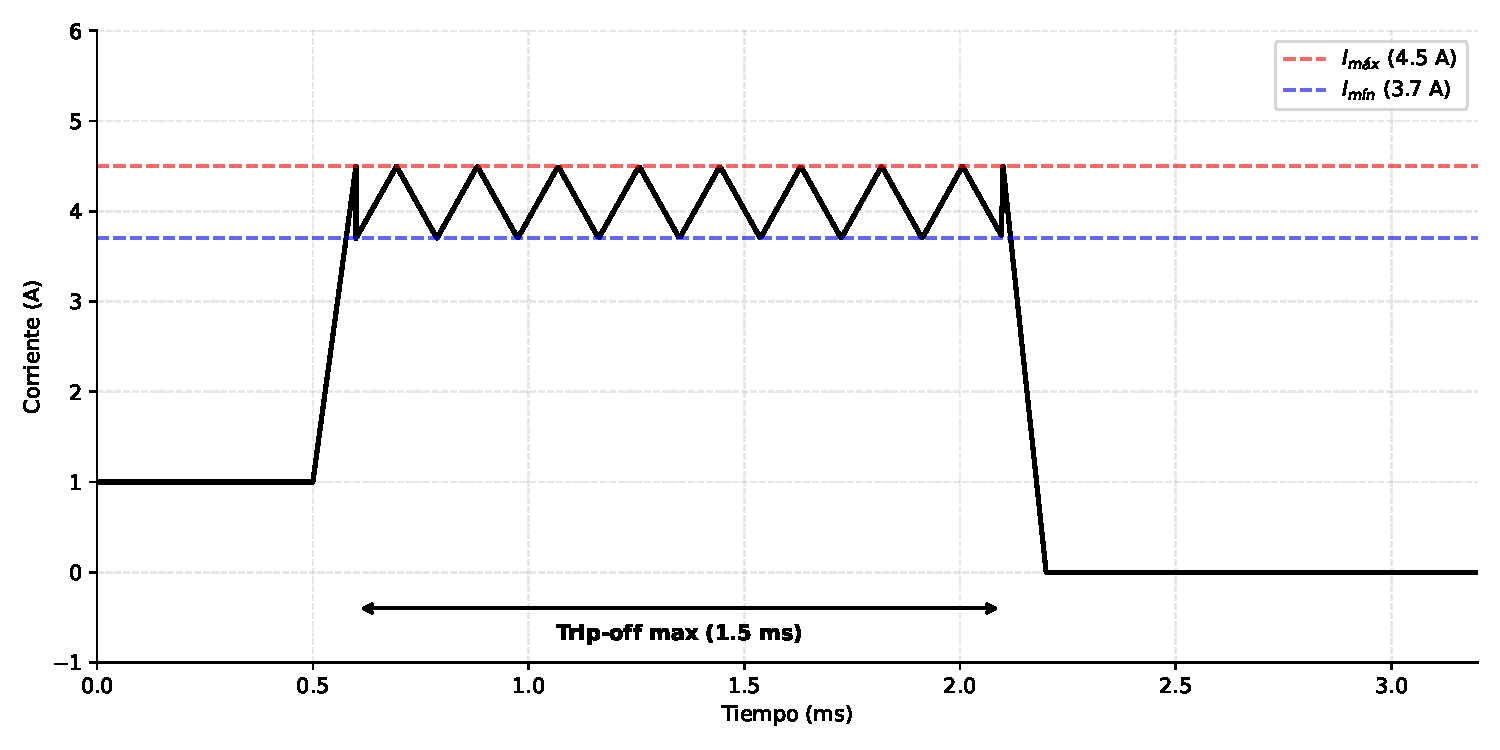
\includegraphics[width=0.8\textwidth]{Histeresis.pdf}
    }
    
    % Añadimos la fuente requerida por tu guía de TFG
    \vspace{2mm}
    {\raggedleft \textbf{Fuente:} Elaboración propia. \par}
\end{figure}
La selección de la amplitud es un \textit{trade-off} entre la frecuencia de conmutación de nuestro limitador y el rendimiento que tendrá térmicamente. A partir de la ecuación \ref{eq:fswitchParasitos} podemos ver que la relación entre la banda de histéresis ($\Delta i$) y la frecuencia de conmutación ($\fswitch$) es inversamente proporcional, lo que supone que, si quisieramos que la fluctuación de corriente fuera menor, tendríamos que aumentar de igual manera la frecuencia de conmutación del N-MOS. Esto como ya hemos visto provocaría un incremento de las pérdidas en conmutación y, por tanto, un mayor estrés térmico, pudiendo salir del Área de Operación Segura del dispositivo. 

Además, la banda no debe ser tan estrecha como para que el tiempo de retardo ($t_\text{sense}$) sea comparable con el tiempo de conmutación ya que, de ser así, se producirían solapamientos y picos de corriente.

\subsubsection{Limite Inferior de Histéresis($\IhistInf$)}
El límite inferior de histéresis se ha seleccionado para que coincida con el valor de la corriente de limitación, es decir, $3{,}7\,A$, por varios motivos. 

Uno de los motivos es la función intrínseca del LCL. Como vimos en la evolución histórica de los limitadores, componentes como los fusibles o los disyuntores se abren inmediatamente al recibir una corriente por encima de un valor determinado mientras los LCL limitan esa corriente durante un cierto tiempo para no desconectar de forma prematura la carga en caso de que sea un simple transitorio. Al fijar el límite inferior en este valor aseguramos que, incluso en el punto más bajo de rizado de conmutación, la carga está recibiendo los $3{,}7\,A$. Por no tener referencias respecto a la carga que se podría emplear en una aplicación real, debemos seleccionar un límite inferior que pueda asegurar el aportar una corriente media suficiente para mantener la carga operativa en los transitorios. 

Otro de los motivos es la lógica implementada en el temporizador. La etapa de temporización emplea un integrado para comparar la caida de voltaje en la resistencia de medida respecto a un voltaje proporcional al paso de $3{,}7\,A$ por esa resistencia. Eligiendo un valor menor, existirían instantes durante la conmutación donde la corriente estaría por debajo del valor de activación del temporizador por lo que el condensador del mismo se empezaría a descargar para volver a cargarse al volver a subir la corriente, provocando que el \textit{trip-off time} fuese mayor de $1{,}5\,ms$.

Además, el rizado debe ser lo suficientemente grande para no llevar a un nivel demasiado alto la frecuencia y, por tanto, no disipar excesivamente en conmutación. Con este objetivo en mente, disminuímos al máximo el valor límite por abajo al provocar menores pérdidas de las que se producirían si aumentasemos el mismo valor el límite superior.
 
\subsubsection{Limite Superior de Histéresis($\IhistSup$)}
La selección del límite superior de $4{,}5\,A$ está integramente relacionada con la banda de histéresis y con el límite inferior que acabamos de ver. 
Como hemos visto, una banda más estrecha provocaría un posible solapamiento entre el tiempo de retardo y el tiempo de conmutación por lo que un valor de $0{,}8\,A$ nos asegura una frecuencia de $614{,}98\,kHz$ que nos separa del tiempo de retraso calculado con valor de $171{,}4\,ns$. De esta manera, aseguramos que tras el \textit{overshoot} inicial la corriente no llegue a valores destructivos para el circuito, como establecimos en el apartado \ref{subsec:inductanciaECSS}. 

Para las clases de 28 voltios de la ECSS, la banda se establece de $0{,}9 \,A$ para la clase de 3 amperios y de $1{,}2\,A$ para la clase de 4 amperios. Para la corriente de limitación de $3{,}7\,A$ la banda será más restrictiva, pues la potencia es más elevada debido al voltaje del bus empleado. Es por ello por lo que, mientras para la clase 4 se llega hasta los $5{,}6\,A$, nosotros para una corriente entre la clase 3 y la clase 4 llegaremos hasta un valor superior más conservador. 

\subsection{Parametrización del temporizador}
El bloque de temporización explicado con anterioridad tiene como objetivo determinar el tiempo máximo ($t_\text{trip}$) durante el cual el limitador permite que la corriente conmute en el rango de histéresis durante la sobrecorriente. Si una vez finalizado este tiempo la corriente no ha bajado a un valor inferior a $3{,}7\,A$ el limitador se enclava y desconecta la carga. 


Fijándonos únicamente en el bloque de temporización de la figura \ref{fig:histeresistemporizacion} obtenemos la siguiente figura más precisa. Los valores de las resistencias y condensador se justificarán a continuación. 

\begin{figure}[H]
    \centering
    \fontsize{10}{12}\selectfont 
    
    \ffigbox[\FBwidth]
    {
        \caption{Parametrización del bloque de temporización}
        \label{fig:temporizadorValores}
    }{
    \begin{tikzpicture}[transform shape]
	% Paths, nodes and wires:
	\node[op amp, xscale=-0.52, yscale=0.52] at (9.231, 10.495){};
	\node[op amp, xscale=-0.52, yscale=0.52] at (14.831, 10.75){};
	\draw (11.55, 10.75) to[empty diode, /tikz/circuitikz/bipoles/length=0.700cm] (12.25, 10.75);
	\node[shape=rectangle, minimum width=1.525cm, minimum height=0.665cm] at (16.112, 10.5){} node[anchor=north west, align=left, text width=1.137cm, inner sep=6pt] at (15.331, 10.85){Vsense};
	\draw (14.131, 10.75) to[american resistor, l={$Rdis=100\,k\Omega$}, label distance=0.04cm] (12.25, 10.75);
	\draw (13.531, 11.55) to[empty diode, /tikz/circuitikz/bipoles/length=0.700cm] (12.431, 11.55);
	\draw (13.531, 11.55) -| (14.031, 10.75);
	\draw (12.281, 11.55) -- (11.581, 11.55) -| (11.5, 10.75);
	\draw (14.131, 10.75) -- (14.431, 10.75);
	\draw (11.731, 10.75) -- (10.731, 10.75);
	\draw (10.731, 10.75) -| (9.85, 10.745);
	\draw (11.5, 9.85) to[capacitor, /tikz/circuitikz/bipoles/length=0.700cm, l={$C_\text{timer}=100\,nF$}, label distance=-0.07cm] (11.5, 8.75);
	\node[sground] at (11.5, 9.05){};
	\draw (8.531, 10.495) -| (8.612, 10.486);
	\draw (14.031, 13.5) -| (14.031, 13);
	\node[ocirc, xscale=-1, yscale=-1](N1) at (14.031, 13.5){} node[anchor=west] at ([xshift=0.09cm]N1.north east){$V_\text{cc}$};
	\draw (14.031, 11.55) to[american resistor, l_={$R3=26{,}1\,k\Omega$}] (14.031, 13.2);
	\draw (8.531, 13.095) -| (8.531, 12.595);
	\node[ocirc, xscale=-1, yscale=-1](N2) at (8.531, 13.095){} node[anchor=west] at ([xshift=0.09cm]N2.north east){$V_\text{cc}$};
	\draw (8.531, 10.495) to[american resistor, l={$R4=5{,}6\,k\Omega$}] (8.531, 12.795);
	\draw (11.5, 10.75) -- (11.5, 10.1);
	\node[shape=rectangle, minimum width=-0.035cm, minimum height=-0.035cm] at (15.231, 9){};
	\node[shape=rectangle, minimum width=2.465cm, minimum height=0.665cm] at (19.25, 7.5){} node[anchor=north west, align=left, text width=2.077cm, inner sep=6pt] at (18, 7.85){Temporizador\\};
	\draw (7.75, 10.5) -| (8.531, 10.495);
	\node[ocirc, xscale=-1, yscale=-1](N3) at (7.75, 10.5){} node[anchor=east] at ([xshift=-0.09cm]N3.east){$V_\text{shutdown}$};
	\draw (17.25, 9.35) to[american resistor, l_={$R2=1{,}1\,k\Omega$}, label distance=-0.09cm] (17.25, 11);
	\draw (17.25, 11) -| (15.45, 11.005);
	\node[sground] at (17.25, 9.35){};
	\draw (17.25, 11.5) -| (17.25, 11);
	\draw (17.25, 13.5) -| (17.25, 13);
	\node[ocirc, xscale=-1, yscale=-1](N4) at (17.25, 13.5){} node[anchor=west] at ([xshift=0.09cm]N4.north east){$V_\text{cc}$};
	\draw (17.25, 11.55) to[american resistor, l_={$R1=1{,}6\,k\Omega$}, label distance=-0.09cm] (17.25, 13.2);
	\draw (17.25, 11.55) -| (17.25, 11.5);
	\draw (11.5, 10.1) -| (11.5, 9.85);
	\draw (9.85, 10.25) -| (10.5, 10.26) |- (20, 8.25) |- (17.25, 11.01);
	\node[circ] at (17.25, 11){};
	\node[ocirc, xscale=-1, yscale=-1](N5) at (20.25, 11){} node[anchor=west] at ([xshift=0.09cm]N5.north east){$V_\text{TimON}$};
	\draw (20.25, 11) |- (20, 11.01);
	\draw (12.431, 11.55) |- (12.281, 11.55);
\end{tikzpicture}
    
   }
    
    \vspace{2mm}
    {\raggedleft \textbf{Fuente:} Elaboración propia. \par}
\end{figure}

La alimentación auxiliar $V_\text{cc}$ de $5\,V$ es la encargada de, a través de un divisor resistivo, establecer el valor a partir del cual el temporizador empieza a funcionar. Este valor será la caída de voltaje equivalente a un paso de la corriente de limitación, $3{,}7\,A$, a través de la resistencia de sensado multiplicada por la ganancia propia de la etapa de sensado, es decir, los $25\,V/V$ que vemos en la ecuación \ref{eq:gananciaSensado}. 

\begin{equation}
    \label{eq:VtimON}
    V_\text{timON} = G_\text{sensado} \cdot I_\text{lim} \cdot R_\text{shunt} = 25 \cdot 3{,}7 \cdot 22\cdot 10^{-3} = 2{,}035\,V
\end{equation}

Para obtener este valor como se expresa arriba, se emplea un divisor resistivo simple con dos resistencias, siendo el voltaje de entrada los $5\,V$ de alimentación y el de salida $V_\text{timON}$. Obtenemos la siguiente ecuación para el cálculo de los valores para las resistencias $R_\text{1}$ y $R_\text{2}$ de la figura \ref{fig:temporizadorValores}:

\begin{equation}
    \label{eq:resistencaisVtimON}
    V_\text{timON}= V_\text{cc} \cdot \frac{R_\text{2}}{R_\text{1} + R_\text{2}}\Rightarrow \frac{R_\text{1}}{R_\text{2}} = \frac{V_\text{cc}}{V_\text{timON}} - 1 \Rightarrow R_\text{1} = 1{,}46 \cdot R_\text{2}
\end{equation}

A partir de esta ecuación y recordando el enfoque práctico que se le busca dar al proyecto, buscaremos dos resistencias que, siguiendo esta relación, sean más comunes. En este caso se decide optar por una $R_\text{UP}$ de $1{,}6\, k\Omega$ y una $R_\text{DOWN}$ de $1{,}1\, k\Omega$. 

Siguiendo el circuito, una vez el voltaje $V_\text{sense}$ llegue a este valor, el comparador en colector abierto cambiará de estado. En un primer momento, la entrada negativa será mayor que la entrada positiva ($V_\text{-} >V_\text{+}$) por no haber una sobrecorriente, lo que hace que el transistor interno se encienda y conecte la salida a tierra. En cambio, cuando se detecta una sobrecorriente la entrada positiva del primer comparador excede los $2{,}035\,V$ ($V_\text{-} <V_\text{+}$) apagando el transistor interno y manteniendo la salida flotante. Gracias a la resistencia \textit{pull-up} denominada $R_\text{3}$ en la figura \ref{fig:temporizadorValores}, la salida es alta y comienza la carga del condensador.  

En este caso, cuando el condensador llegue a cargarse por encima del valor $2{,}035\,V$ cambiará el estado del segundo comparador. A diferencia del anterior comparador, el valor de referencia está conectado a la entrada positiva por lo que en un primer momento esta será mayor que la entrada negativa ($V_\text{+} >V_\text{-}$) manteniendo la salida alta gracias a la resistencia \textit{pull-up} R4. Si volvemos a la topología de la figura \ref{fig:histeresistemporizacion} vemos que esto hace que en la entrada de la puerta \textit{AND} haya un ``1'' lógico, permitiendo que se produzca la conmutación controlada por el bloque de histéresis. 
Una vez el voltaje en el condensador sea tal que el tiempo de limitación se ha agotado, el transitor del comparador se encenderá llevando la salida a tierra, lo que implica un ``0'' lógico en la puerta \textit{AND} y, por tanto, el enclavamiento. 

Para facilitar el seguimiento de la lógica del temporizador se presenta la siguiente tabla (\ref{table:estados_driver}) con los posibles estados del temporizador:

\begin{table}[H]
    \centering
    \fontsize{10}{12}\selectfont
    \ttabbox[\textwidth]
    {\caption{ANÁLISIS LÓGICO DEL BLOQUE DE TEMPORIZACIÓN SEGÚN LA TENSIÓN $V_{SENSE}$ Y EL TIEMPO}}
    {\begin{tabular}{|P{2cm}|P{1.8cm}|P{3.5cm}|P{3.5cm}|P{3.2cm}|}
        \hline
        \textbf{Valor $V_{SENSE}$ (V)} & \textbf{Tiempo (ms)} & \textbf{Estado Transistor Comparador 1} & \textbf{Estado Transistor Comparador 2} & \textbf{Lógica de Salida} \\
        \hline
        $< 2{,}035$ & --- & Activo (GND en salida) & Inactivo ($V_{CC}$ en salida) & "1" (Driver habilitado) \\
        \hline
        $> 2{,}035$ & $< 1{,}5$ & Inactivo ($V_{CC}$ en salida) & Inactivo ($V_{CC}$ en salida) & "1" (Driver habilitado) \\
        \hline
        $> 2{,}035$ & $> 1{,}5$ & Inactivo ($V_{CC}$ en salida) & Activo (GND en salida) & "0" (Driver deshabilitado) \\
        \hline
        \multicolumn{5}{r}{\rule{0pt}{3ex}\textbf{Fuente:} Elaboración propia}
        \label{table:estados_driver}
    \end{tabular}}
\end{table}


Para que nuestro temporizador siga los requisitos que le hemos impuesto debemos fijarnos en la red RC de carga y descarga del condensador la cual es asimétrica, lo que significa que cuenta con distintas constantes temporales ($\tau$) para ambos casos.

\subsubsection{Carga del condensador}
El objetivo del temporizador es, cuando hay una sobrecorriente, cargar un condensador hasta un valor tal que, una vez se haya llegado, hayan pasado $1{,}5\,ms$. Debido a que ya tenemos un divisor resistivo calculado para darnos $2{,}035 \,V$, podemos reutilizar este valor como voltaje al que se habrá cargado el condensador tras el \textit{trip-off time}.     

En la subsección \ref{subsec:temporizador} donde se explica la topología del temporizador, se presenta la ecuación \ref{eq:cargaCondensador} con la fórmula que rige la carga de un condensador. Como se ha expresado anteriormente, con el objetivo de no repetir de manera innecesaria cálculos se emplean valores reales como es el caso de la caída de voltaje provocada por el diodo. A partir de la ecuación de carga incluímos el voltaje del diodo: 

\begin{equation}
    \label{eq:cargaCondensadorTau}
    V_\text{timON} = (V_\text{cc}-V_\text{F}) \cdot \left(1 - e^{-\frac{t}{\tau_\text{carga}}}\right)
\end{equation}

Operando la anterior ecuación e incluyendo los valores llegamos a obtener la constante de carga ($\tau_\text{carga}$): 
\begin{equation}
    \label{eq:tauCarga}
    \tau_\text{carga} = - \frac{t_\text{trip}}{ln\left(1 - \frac{V_\text{timON}}{V_\text{cc}-V_\text{F}}\right)} = - \frac{1{,}5\cdot 10^{-3}}{ln\left(1 - \frac{2{,}035}{5-0{,}32}\right)} = 2{,}61 \cdot 10^{-3}
\end{equation}

Habiendo obtenido este valor y sabiendo que la constante de tiempo de una red RC es el producto de ambas podemos seleccionar uno de ambos componentes y ajustar el otro. Se emplea un condensador de $100\, nF$ por ser este valor un \textit{trade-off} entre protección ante capacidades parásitas que no tendríamos con un condensador de poco valor y un tiempo de respuesta aceptable que no tendríamos con uno de alto valor. Además, este valor nos lleva al uso de una resistencia \textit{pull-up} encargada de la carga de $26{,}1\,k\Omega$, valor comercial y con corrientes de fuga mínimas. 


\subsubsection{Descarga del condensador}
La red asimétrica se implementa con el objetivo de dotar al circuito temporizador de memoria para que, si dos sobrecorrientes de las cuales la primera es menor de $1{,}5\, ms$ se suceden en un muy corto periodo de tiempo, el temporizador tenga en cuenta que el transistor no ha tenido tiempo a enfriarse. De no implementarse este mecanismo, el permitir una segunda sobrecorriente que durase todo el tiempo de \textit{trip-off} podría excederse la temperatura máxima del N-MOS y perder el dispositivo. 

A partir de la hoja de datos del fabricante para el N-MOS IRFB4020PBF \cite{noauthor_irfb4020pbfpmd_nodate}, podemos ver en la figura \ref{fig:Foster} la red térmica de Foster donde se muestran cada una de las capas internas que conforman el dispositivo. 

\begin{figure}[H]
    \centering
    % Forzamos 10pt para cumplir con la normativa de tu guía
    \fontsize{10}{12}\selectfont 
    \ffigbox[\FBwidth]
    {
        \caption{Impedancia térmica del N-MOS}
        \label{fig:Foster}
    }
    {
        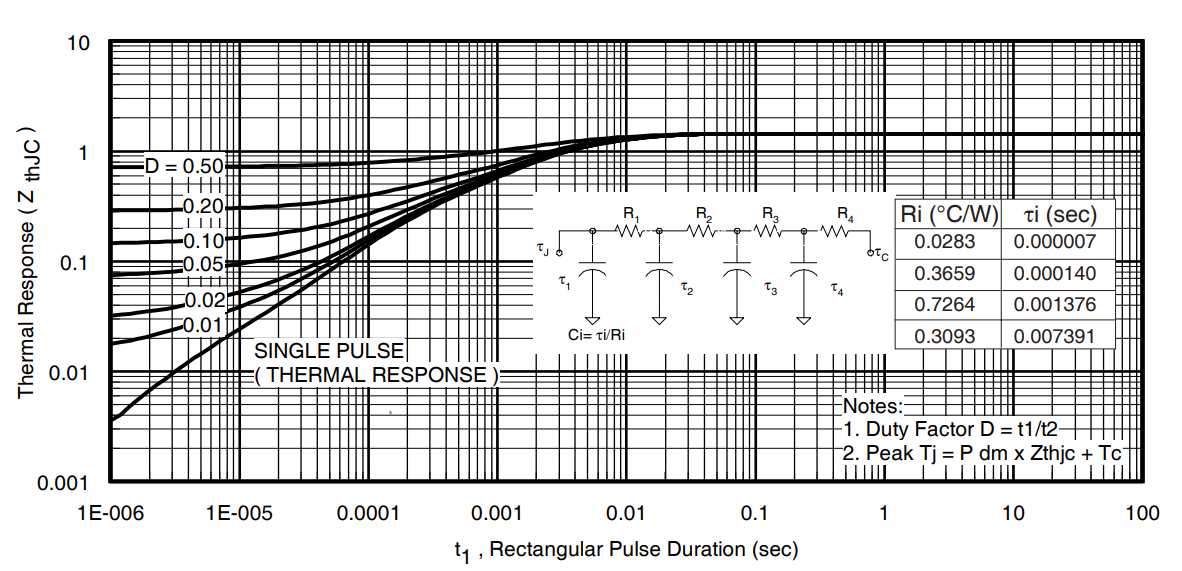
\includegraphics[width=0.8\textwidth]{foster.png}
    }
    
    % Añadimos la fuente requerida por tu guía de TFG
    \vspace{2mm}
    {\raggedleft \textbf{Fuente:} Extraído de la hoja de datos de Infineon para el IRFP9240PBF\cite{noauthor_irfb4020pbfpmd_nodate}. \par}
\end{figure}

En la imagen se especifica, para cada una de las capas del semiconductor, la constante de tiempo asociada, siendo la más grande $\tau_\text{4}$ con un valor de $0{,}007391$ segundos. Por ser la más restrictiva será en la que nos basaremos para calcular cuanto tardará el transistor en enfriarse. 

Para el análisis térmico transitorio consideramos el sistema de primer orden asumiendo, por tanto, que se consigue un enfriamiento prácticamente completo tras un intervalo de tiempo de 5 veces su constante de tiempo, es decir, tras al menos $36{,}955$ milisegundos. Siendo el estrés térmico el factor que más puede afectar a nuestro transistor se ha buscado ser conservador con el enfriamiento seleccionando una resistencia de $100\,k\Omega$. Con este valor, el tiempo disponible de memoria térmica del sistema vendrá dado por la siguiente ecuación:\begin{equation}
    \label{eq:tauDescarga}
    t_\text{descarga} = 5\cdot C_\text{timer} \cdot (R_\text{3}+R_\text{dis})=5\cdot 100\cdot 10^{-9} \cdot (26{,}1 \cdot 10^{-3}+ 100\cdot 10^{-3}) = 63{,}05\, ms
\end{equation}

Este resultado indica que, durante los $63{,}05\, ms$ posteriores a una sobrecorriente que no termina en enclavamiento por no superar el tiempo máximo, el sistema asumirá que el transistor está enfriándose y protegerá su integridad disminuyendo el tiempo de limitación de corriente antes del enclavamiento. Cuanto menos espaciadas estén dos sobrecorrientes, mayor será el voltaje restante en el condensador y más cercano estará de superar el valor que hace que el sistema se enclave. 


\subsection{Diseño del filtrado de entrada ($C_{bus}$)}
Los condensadores empleados a la entrada de un limitador de corriente conmutado sirven como sistema de filtrado con doble objetivo: servir de reserva de energía (Condensador \textit{Bulk}) manteniendo un valor de bus estable en caso de variaciones de carga o del propio valor del bus, y reducir el ruido inducido por la conmutación a alta frecuencia del MOSFET. Para lograr ambos objetivos es necesario contar con un condensador capaz de tener alta capacitancia y velocidad de respuesta, siendo difícil encontrar un condensador óptimo para ambos intereses. 

Es por ello por lo que se decide emplear dos condensadores en paralelo entre bus y masa, cada uno con su ubicación en el prototipo y con un objetivo marcado. 
\subsubsection{Condensador de almacenamiento o \textit{Bulk}}
El primer filtrado consiste en un condensador electrolítico de $47\text{ }\mu\text{F}$ que deberemos situar físicamente a la entrada del circuito, lo más cercano posible de los conectores de alimentación del bus. Para el dimensionado del mismo debemos tener en cuenta dos factores, la respuesta dinámica y la seguridad contra corrientes de inserción de nuestro circuito, lo que determinará un límite inferior y un límite superior respectivamente. 
\begin{itemize}
    \item \textbf{Límite inferior: }Establecemos este límite inferior en aproximadamente $10\text{ }\mu\text{F}$ para asegurar que el tiempo de respuesta del control en caso de falla no provoque una gran caída en el voltaje del bus.
    \item \textbf{Límite superior: }Establecemos este límite superior en aproximadamente $100\text{ }\mu\text{F}$ debido a que, de establecer un valor mayor, una excesiva corriente de inserción (\textit{inrush current}) provocada por el encendido podría ser vista como un cortocircuito en vez de una funcionalidad deseada. 
\end{itemize}
Con ambos límitese en mente, se opta por $47\text{ }\mu\text{F}$ para proteger el circuito de una pérdida de la capacidad del condensador que nos llevaría a situarnos por debajo del valor límite inferior, y para situarnos debajo del límite superior siendo capaces de mantener una reserva de energía lo suficientemente grande como para mantener el voltaje del bus en un valor constante sin arriesgarnos a problemas con la mencionada corriente de arranque. 

\subsubsection{Condensador de alta frecuencia}
El segundo filtrado consiste en un condensador de $1\text{ }\mu\text{F}$ que deberá tener una baja inductancia serie equivalente (ESL) para poder actuar a alta frecuencia. Debido a la alta frecuencia de conmutación empleada, el condensador \textit{bulk} empleado para almacenar energía no es capaz de gestionar la necesidad de flancos de corriente del semiconductor por tener una alta ESL. Es por ello por lo que se decide emplear este segundo condensador, en este caso cerámico, que deberá estar situado lo más cercano posible al transistor. Al igual que en el caso anterior, se tienen en cuenta dos factores que establecen límites para la selección de los componentes, siendo estos factores la capacitancia y la respuesta a alta frecuencia.

Se ha seleccionado el valor de $1\text{ }\mu\text{F}$ debido a que valores menores podrían no tener suficiente energía para evitar los problemas causados por el pico de corriente, mientras que a medida que aumentaramos el valor de capacitancia nos iríamos encontrando con valores de ESL mayores, lo que haría que la respuesta fuera cada vez más lenta, inhabilitando la función principal del componente.

La cercanía de este componente al drenador del MOSFET hace que el bucle de conmutación se cierre en un área mínima, lo que aumenta la velocidad y, por ser menor la distancia de las vías, disminuye la inductancia parásita que a su vez disminuiría la velocidad. La cercanía hace que las sobretensiones producidas en el apagado del N-MOS se vean reducidas, asegurando la protección y estabilidad del circuito y componentes. 

\subsubsection{Rizado de tensión en el bus}
La justificación teórica nos lleva a los valores descritos de $47\text{ }\mu F$ y $1\text{ }\mu F$ pero es el cálculo del rizado de tensión en el bus lo que nos determina si la teoría se adecúa a lo que buscamos. Como se calculó en la subsección \ref{subsec:Cálculo de la frecuencia de conmutación}, la frecuencia de conmutación para el peor caso será de $614{,}98\,kHz$, la propia de un ciclo de trabajo del $50\%$. El rizado, considerando la capacitancia total del sistema con los dos condensadores, viene dada por la ecuación \ref{eq:rizadotensionbusCondensador}:
\begin{equation}
    \label{eq:rizadotensionbusCondensador}
    \Delta V_\text{bus} = \frac{I_\text{out} \cdot D \cdot (1 - D)}{f_\text{sw} \cdot C_\text{total}} = \frac{3{,}7 \cdot 0{,}5 \cdot (1-0{,}5)}{614{,}98 \cdot 10^{3}\cdot (47\cdot 10^{-6} + 1 \cdot 10^{-6})} = 31{,}3 \text{ mV}
\end{equation}

Un rizado de 31,3 mV supone únicamente un $0{,}031\%$ de la tensión nominal de $100\text{ V}$, estando a su vez lejos de la caída de voltaje propia del paso de $3{,}7\text{ A}$. Por tanto, con estos valores se garantiza un bus estable y seguro cumpliendo con los requisitos determinados a lo largo del capítulo. 
\section{Síntesis de los valores principales}   
Una vez realizado todo el desarrollo analítico y matemático del capítulo, la síntesis del mismo busca integrar de forma sencilla los requisitos de la normativa ECSS junto a los límites de los componentes seleccionados. Como resultado del desarrollo analítico y matemático presentado en este capítulo, se propone una consolidación paramétrica que integra los requisitos normativos de la normativa ECSS adaptada con los límites físicos del. 

Para entender correctamente el operatividad de un limitador conmutado en un bus de alta tensión de 100 V, es necesario realizar el estudio del comportamiento no únicamente individual de cada etapas, tanto de control como de potencia, sino que es preciso visualizarlo desde la perspectiva común que une cada una de ellas, es decir, la relación entre las constantes eléctricas, las frecuencias del sistema de control y los límites térmicos del semiconductor de potencia N-MOS. 

Con el objetivo de facilitar la visualización, la Tabla \ref{table:ResumenTeoria} ofrece una estructuración de los valores numéricos definitivos y las reglas de decisión para las nueve áreas principales que regulan el sistema. Esta tabla incluye desde los requisitos de la carga hasta las condiciones dinámicas del bus asimétrico del temporizador y el filtro en dos fases de entrada. De esta manera, se asegura que el limitador tenga una base consistentepara enfrentarse a escenarios de cortocircuitosevero  y se proporciona un marco cuantitativo que actuará como punto de partida para los cálculos parásitos de la próxima fase numérica.

\begin{table}[H]
    \centering
    \fontsize{10}{12}\selectfont
    \ttabbox[\textwidth]
    {\caption{SÍNTESIS DE LOS VALORES PRINCIPALES Y PARÁMETROS DE DISEÑO DEL LCL CONMUTADO (100 V)}}
    {\begin{tabular}{|P{3.2cm}|P{3.5cm}|P{5.8cm}|}
        \hline
        \textbf{PARÁMETRO / CATEGORÍA} & \textbf{VALORES OBTENIDOS} & \textbf{CRITERIO DE SELECCIÓN} \\
        \hline
        Especificaciones del bus y de la carga & 
        $V_\text{bus} = 100\text{ V}$ \newline 
        $I_\text{lim} = 3{,}7\text{ A}$ \newline 
        $t_\text{trip} = 1{,}5\text{ ms}$ & 
        Límites del prototipo, empleando el tiempo de disparo más restrictivo de las clases de 28 V debido al incremento de potencia disipada. \\
        \hline
        Banda de histéresis de corriente & 
        $I_\text{hys,sup} = 4{,}5\text{ A}$ \newline 
        $I_\text{hys,inf} = 3{,}7\text{ A}$ \newline 
        $\Delta i = 0{,}8\text{ A}$ & 
        El límite inferior coincide con $I_\text{lim}$ para garantizar la corriente suficiente a la carga y el ancho de banda evita el solapamiento por retardos del sensado. \\
        \hline
        Etapa de sensado y acondicionamiento & 
        $R_\text{shunt} = 22\text{ m}\Omega$ \newline 
        $P_\text{shunt} = 0{,}3012\text{ W}$ \newline 
        $G \approx -25\text{ V/V}$ \newline
        $V_\text{sense} = 2{,}035\text{ V}$ & 
        Minimización de pérdidas térmicas por efecto Joule asegurando una alta relación señal-ruido (SNR). \\
        \hline
        Límites térmicos del semiconductor & 
        $T_\text{j,max} = 125\text{ }^\circ\text{C}$ \newline 
        $P_\text{mos,max} = 10{,}07\text{ W}$ \newline 
        $f_\text{sw,max} \le 2{,}253\text{ MHz}$ & 
        Temperatura de seguridad fijada por la hoja de datos y potencia máxima obtenida mediante red térmica equivalente con disipador. \\
        \hline
        Dimensionado del inductor ($L$) & 
        $L_\text{min1} = 3{,}116\text{ }\mu\text{H}$ \newline 
        $L_\text{min2} = 1{,}7\text{ }\mu\text{H}$ \newline 
        $L_\text{min3} = 42{,}85\text{ }\mu\text{H}$ \newline 
        $L_\text{seleccionada} = 68\text{ }\mu\text{H}$ & 
        Evaluación de las 3 condiciones de la ECSS adaptadas y ajuste a la más restrictiva mediante valor comercial. \\
        \hline
        Frecuencia operacional del lazo & 
        $f_\text{sw} = 614{,}98\text{ kHz}$ & 
        Frecuencia teórica resultante para el peor escenario operacional con ciclo de trabajo del 50\% ($V_\text{out} = 50\text{ V}$). \\
        \hline
        Parámetros del temporizador RC & 
        $C_\text{timer} = 100\text{ nF}$ \newline 
        $R_3 = 26{,}1\text{ k}\Omega$ \newline 
        $\tau_\text{carga} = 2{,}61\cdot10^{-3}$ & 
        Divisor resistivo fija el umbral de disparo en $V_\text{timON} = 2{,}035\text{ V}$. \\
        \hline
        Memoria térmica de descarga & 
        $R_\text{dis} = 100\text{ k}\Omega$ 
        \newline 
        $t_\text{descarga} = 63{,}05\text{ ms}$ & 
        Red asimétrica de descarga basada en la constante de tiempo térmica de la capa interna más lenta del NMOS. \\
        \hline
        Filtro de entrada del bus & 
        $C_\text{bulk} = 47\text{ }\mu\text{F}$  \newline 
        $C_\text{HF} = 1\text{ }\mu\text{F}$  \newline 
        $\Delta V_\text{bus} = 31{,}3\text{ mV}$ & 
        Configuración en paralelo que combina almacenamiento de energía bulk con baja ESL para alta frecuencia. \\
        \hline
        \multicolumn{3}{r}{\rule{0pt}{3ex}\textbf{Fuente:} Elaboración propia a partir de los modelos  analizados en el Capítulo 3.}
        \label{table:ResumenTeoria}
    \end{tabular}}
\end{table}



\chapter{Elección de componentes e implementación en psim con parásitas de los componentes seleccionados}
Una vez realizado el dimensionamiento y análisis teórico del circuito debemos trasladar lo observado a la realidad de nuestra aplicación. En el anterior capítulo se presentaron ciertos valores parásitos de los componentes a usar sin justificar la elección de los mismos para no repetir los cálculos en el caso ideal y con elementos parásitos. 

El presente capítulo se divide en dos fases. Durante la primera fase se justifican las especificaciones buscadas para los componentes más críticos  del dispositivo y los componentes comerciales elegidos para el protótipo físico del laboratorio. Posteriormente, se mostrará la implementación del circuito en la herramienta de simulación PSIM, incluyendo los modélos parásitos obtenidos de las hojas de características de los fabricantes para validar el comportamiento dinámico y comprobar que los cálculos realizados para obtener el \textit{trip-off time} y los límites de histéresis deseados han sido correctos. 

\section{Justificación de los componentes seleccionados}
El propósito de la sección es justificar qué dispositivos comerciales disponibles en distribuidores de renombre como Mouser o DigiKey se han seleccionado para realizar este primer prototipo del LCL conmutado. Como se ha ido remarcando durante el trascurso del documento, el diseño se entiende como una primera aproximación o prueba para validar el funcionamiento de la topología en un entorno de laboratorio controlado. Es por esto por lo que se ha priorizado emplear componentes comerciales disponibles en el momento del montaje de la placa frente a dispositivos con calificación espacial los cuales, además de incrementar enormemente el precio del prototipado, obligarían en el momento de su elección a tener en cuenta ciertos parámetros como la inmunidad a radiación, encapsulados... que quedan fuera del objetivo del trabajo. 

Para facilitar el replicamiento del prototipo, la lista de materiales detallada con las referencias de los fabricantes y encapsulados se encuentra disponible en el Anexo [1].
\subsection{MOSFET de potencia: IRFB4020PbF}
El elemento principal del limitador, es decir el MOSFET de potencia, debe justificar la selección de esta topología y ensalzar la mejora que supone tanto el uso de los MOSFET de canal N como la limitación por conmutación que se ha justificado durante el documento. Es por esto por lo que se ha seleccionado el transistor \textit{IRFB4020PbF} de Infineon (International Rectifier) \cite{noauthor_irfb4020pbfpmd_nodate}.

Este dispositivo, fabricado en Silicio, presenta las principales características siguientes: 
\begin{itemize}
    \item \textbf{Tensión drenador-fuente:} permite un máximo de 200V, lo que supone un margen del $100\%$ respecto a la tensión del bus nominal. 
    \item \textbf{Corriente en el drenador:} permite el paso continuo de $18\text{ A}$ con pulsos máximos de $52\text{ A}$, lo que supone un orden de seguridad perfecto respecto al máximo permitido del limitador durante un pulso ($10\text{ A}$) o durante la limitación ($4{,}5\text{ A}$).
    \item \textbf{Resistencia en conducción: } el transistor cuenta con una resistencia en conducción relativamente alta ($\rdson = 80 \text{m}\Omega$) en comparación con otras alternativas por el interés de mejorar la respuesta dinámica en detrimento de las pérdidas por conducción.
    \item \textbf{Carga de puerta:} por lo mencionado anteriormente, se ha seleccionado este N-MOS teniendo en cuenta el bajo valor de carga de la puerta ($Q_\text{G} = 18 \text{nC}$). Esto permite un rápido cambio de estado del transistor y pocas perdidas en la conmutación. 
\end{itemize}

Al compararlo con distintos transistores de Silicio, el \textit{IRFB4020PbF} presenta una ventaja principal que justifica su selección para el lazo de conmutación de alta frecuencia. Los distintos transistores disponibles no contaban con una relación entre pérdidas por conducción y pérdidas por conmutación tan óptima para la aplicación al estar principalmente ideados para la conducción. 
Estas opciones cuentan con una resistencia en conducción mucho menor, pero sus pérdidas de conmutación se disparan enormemente. Teniendo en cuenta la corriente que fluye de forma nominal por el circuito, las pérdidas por conducción son gestionables por el transistor sin sufrir estrés térmico excesivo, y la caída de voltaje es nimia en un bus de 100 voltios. 

Por otro lado, a pesar de habernos centrado durante el Capítulo 2 en las propiedades físicas de los materiales de banda prohibida ancha como el Carburo de Silicio o el Nitruro de Galio, por la aplicación concreta y al ser un prototipo incial se ha considerado que la selección de un transistor convencional de Silicio cumple con los requerimientos. 
Debido a normativas o requisitos técnicos, el margen del $100\%$ respecto a la tensión del bus nominal puede no ser suficiente por lo que emplear un transistor de Carburo de Silicio puede ser necesario, pero estos requisitos no influyen en las pruebas iniciales en el laboratorio. Además, el precio de estos transistores es elevado para un prototipado incial y la circuitería necesaria para disparar estos transistores más compleja, dificultando la fuente flotante de la placa de circuito impreso. 



\subsection{Controlador de puerta: UCC27511AQDBVRQ1}
La alta frecuencia de conmutación del MOSFET seleccionada para el prototipo requiere una inyección y extracción rapida en la puerta del mismo. Pese a manejar la lógica del sistema correctamente, las etapas analógicas implementadas no son capaces de aportar la corriente necesaria para el transistor al ritmo deseado. Es por ello por lo que se implementa el controlador de puerta de alta velocidad \textit{UCC27511AQDBVRQ1} de Texas Instruments \cite{texas_instruments_ucc27511a_nodate}.

La elección de este controlador se centra en las siguientes características obtenidas de su hoja de datos:

\begin{itemize}
    \item \textbf{Corriente asimétrica de pico:} el integrado es capaz de entregar una corriente de hasta $4\text{ A}$ durante el encendido y absorber hasta $8\text{ A}$ durante el apagado. Esto permite que el tiempo necesario para el llenado de la carga de puerta del N-MOS se reduzca y, por otro lado, la alta capacidad de absorición evita un posible reencendido por efecto Miller \cite{noauthor_efecto_nodate}.
    \item \textbf{Configuración de salida dividida:} el dispositivo cuenta con pines diferenciados para el encendido (\textit{OUTH}) y el apagado (\textit{OUTL}), permitiendo seleccionar mediante resistencias externas la velocidad de conmutación. 
    \item \textbf{Retardo de propagación:} El \textit{UCC27511A-Q1} cuenta con un retardo interno de propagación típico de  $13\text{ ns}$, con tiempo de subida de $8\text{ ns}$ y de bajada de $7\text{ ns}$. Un valor tan reducido dentro del límite establecido de $171{,}4\text{ ns}$ permite mayor flexibilidad a la hora de seleccionar los comparadores. 
\end{itemize}

\subsection{Diodo de libre conducción: STPSC6H065B-TR}
Durante el tiempo de apagado del N-MOS en la banda de histéresis, la energía magnética almacenada en el inductor obliga a emplear un diodo de libre conducción para que la sobretensión no supere la tensión máxima entre drenador y fuente del MOSFEET y se produzca una rotura por avalancha del semiconductor. 
Con este fin se ha seleccionado el diodo Schottky \textit{STPSC6H065B-TR} de STMicroelectronics \cite{stmicroelectronics_stpsc6h065_nodate}, el cual está hecho de Carburo de Silicio. Este diodo se caracteriza por soportar hasta $650\text{ V}$ y $6\text{ A}$ de forma repetida. 

A pesar de haber empleado el Silicio en el MOSFET por el \textit{trade-off} entre dificultad técnica añadida, precio y beneficios en la etapa de desarrollo actual, el empleo del SiC se justifica en el diodo por los siguientes motivos:

\begin{itemize}
    \item \textbf{Recuperación inversa ($Q_\text{rr} \approx 0$):} por ser un diodo Schottky de SiC se trata de un dispositivo que emplea portadores, por lo que no sufre de la carga de recuperación inversa de los diodos bipolares de Silicio. Durante la conmutación de alta frecuencia, los diodos tradicionales producen una corriente inversa al encender el MOSFET, lo que produciría un aumento en las pérdidas de conmutación del transistor y podría provocar falsos disparos del LCL. Por su parte, el diodo de Carburo de Silicio elimina este transitorio. 
    \item \textbf{Elevado margen de seguridad contra tensiones transitorias:} debido a su alta tensión inversa máxima, el margen de operación respecto al bus nominal es del 550\%. Esto nos permite progeger el sistema frente a los picos de tensión del inductor y evita el uso de redes encargadas de la amortiguación como podrían ser los \textit{snubbers}.
\end{itemize}
\subsection{Comparadores analógicos: LM319AM/NOPB y LM393BIDR}
El lazo de control del limitador de corriente conmutado está formado por dos etapas de comparación distinguidas entre si: el bloque de histéresis encargado de mantener la corriente dentro de la banda y el bloque de temporización encargado de contabilizar el \textit{trip-off time}. 

Debido a las distintas necesidades de ambos bloques, se ha seleccionado cada comparador teniendo en cuenta las restricciones temporales presentes para optimizar la respuesta dinámica. Se empleará por tanto el comparador de alta velocidad \textit{LM319AM/NOPB} y del comparador de bajo consumo \textit{LM393BIDR}

\subsubsection{Bloque de control por histéresis: LM319AM/NOPB}
El bloque de histéresis trabaja en alta frecuencia ($f\approx 615\text{ kHz}$) con el rizado de la corriente permitido. En el Capítulo 3 se mostró como objetivo disminuir el retardo del lazo de control ($t_{sense}$) lo máximo posible para responder rápidamente a la sobrecorriente y evitar que supere los límites de seguridad por los picos producidos durante los transitorios. 

Con esto en mente se ha seleccionado el \textit{LM319AM/NOPB} de Texas Instruments \cite{texas_instruments_lmx19_nodate}, comparador analógico de alta velocidad y dos canales con las siguientes características: 
\begin{itemize}
    \item \textbf{Tiempo de respuesta:} el retardo del comparador es de tan solo $70\text{ ns}$, lo que permite una buena respuesta dinámica frente a la conmutación de la señal de corriente. Además, este buen tiempo de respuesta permite flexibilidad para el OPAMP de sensado y el \textit{driver} del MOSFET, y garantiza la conmutación del transistor antes de la saturación de la bobina. 

    \item \textbf{Flexibilidad de alimentación y salidas en colector abierto:} la tensión de alimentación flexible permite que la fluctuación del voltaje del bus, señal de la cual se obtiene la alimentación de los integrados, no impidan que actue el comparador. Además, la salida en colector abierto permite enviar la señal de control directamente al driver sin la necesidad de integrados intermedios que traduzcan el valor del voltaje. 

\end{itemize}

\subsubsection{Bloque del temporizador de seguridad: LM393BIDR}
A diferencia del anterior bloque, el temporizador actúa en una escala temporal mucho menos restrictiva, teniendo que contabilizar un tiempo de $1{,}5\text{ ms}$ frente a los $1{,}6\text{ }\mu\text{s}$ del circuito de histéresis. Es por ello por lo que el empleo de un comparador de alta velocidad como el \textit{LM319} sería un error de sobrediseño que provocaría un incremento del consumo de energía y coste del sistema, y se emplea un comparador dual general como es el \textit{LM393BIDR} de Texas Instruments \cite{texas_instruments_lm393b_2026}. 

Los principales motivos para su selección son los siguientes: 
\begin{itemize}
    \item \textbf{Consumo energético:} el LCL es un sistema de seguridad que en funcionamiento normal debe pasar inadvertido. Es por eso que durante estos largos tiempos de espera es clave un componente con un bajo consumo como el \textit{LM393BIDR}, teniendo una corriente de alimentación de apenas $200\ \mu\text{A}$ por comparador.
    \item \textbf{Retardo despreciable:} el \textit{LM393B} tiene un tiempo de respuesta de $1\ \mu\text{s}$, el cual es un valor insuficiente para la etapa de histéresis, pero que dentro del temporizador de $1{,}5\text{ ms}$ ($1500\ \mu\text{s}$) supone un retraso marginal en el compromiso entre protección y coste, y tiempo de respuesta.
\end{itemize}


    
\subsection{Inductor de potencia: WE-HCI 74435586800}
El almacenamiento de energía magnética y el filtrado del rizado de corriente a alta frecuencia está gestionado por la bobina de potencia \textit{WE-HCI 74435586800} de Würth Elektronik \cite{wurth_elektronik_74435586800_nodate}. Este componente se ha seleccionado tras los cálculos realizados en el Capítulo 3 que recomendaban una inductancia nominal de $68\ \mu\text{H}$ debido a su comportamiento estable que mantiene la inductancia en el rango de los $66\ \mu\text{H}$ bajo corriente nominal.

La selección de este componente frente a opciones de núcleo toroidal con bobinado a mano se justifica con los siguientes factores:

\begin{itemize}
    \item \textbf{Mitigación de efectos de alta frecuencia por tecnología \textit{Flat Wire}:} el inductor seleccionado emplea conductor plano a diferencia del clásico hilo circular. Para la frecuencia de conmutación seleccionada, el efecto pelicular \cite{noauthor_efecto_nodate-1} y el efecto de proximidad \cite{javier_fernandez_de_sevilla_galan_perdidas_2019} provocan un incremento de la resistencia de la bobina en corriente alterna. Por este motivo se emplea hilo plano el cual optimiza la relación entre el área de la superficie y el volumen, lo cual permite mantener una perdias por efecto Joule reducidas durante la conducción. 
    
    \item \textbf{Saturación suave (\textit{Soft Saturation}):} el material del núcleo (\textit{Manganese Zinc (MnZn) Ferrite}) permite una transición no abrupta que da estabilidad al lazo de control. Ante el pico de corriente, el núcleo evita que la pendiente de la misma aumente hasta ser peligrosa para el sistema antes de la actuación de los comparadores de histéresis. 
    
    \item \textbf{Compatibilidad electromagnética (EMI):} el encapsulado metálico apantallado es clave en un ambiente que opera con señales de bajo nivel (\textbf{81.4 mV} en la resistencia de \textit{shunt}) debido a que cualquier acoplamiento o interferencia provocaría ruido electromagnético en las pistas de la placa. Gracias al apantallamiento interior, el flujo magnético que influye en el exterior es residual, evitando falsos disparos del sistema. 
\end{itemize}
\subsection{Amplificador operacional: OPA2836QDGKRQ1}
El bajo de valor de la resistencia de sensado provoca una caída de tensión de baja amplitud que se podría ver afectada por acoplamiento magnético de otras señales. Es por ello por lo que, antes de realizar la comparación para el ciclo de histéresis, es necesario el acondicionamiento de la señal. Con este objetivo se ha seleccionado el amplificador operacional doble de bajo consumo y banda ancha \textit{OPA2836QDGKRQ1} de Texas Instruments \cite{texas_instruments_opa2836qdgkrq1_nodate}. 

La justificación de este semiconductor viene dada principalmente por los parámetros dinámicos que presenta y que nos permiten llegar a un tiempo de sensado de únicamente $171{,}4\text{ ns}$:

\begin{itemize}
    \item \textbf{Ancho de banda y velocidad de respuesta:} el ancho de banda del \textit{OPA2836} es de $205\text{ MHz}$ con un \textit{Slew Rate} de $560\text{ V}/\mu\text{s}$. La corriente triangular de alta frecuencia que fluye por la inductancia cuenta con pendientes pronunciadas por lo que amplificadores operacionales generales retrasarían la llegada de la señal al temporizador y al controlador de histéresis. La respuesta dinámica de este dispositivo garantiza que la salida de la misma sea una reproducción amplificada pero fidedigna de la señal de entrada.
    \item \textbf{Mínimo retardo temporal:} el integrado seleccionado cuenta con un tiempo de subida de únicamente $3\text{ ns}$ y un bajo tiempo de asentamiento (señal al 0.1\%) de $22\text{ ns}$. Esta respuesta temporal es clave para obtener el \textit{sense time} de $171{,}4\text{ ns}$ que asegura que no se prouzca un retraso en el apagado del MOSFET que pueda provocar la pérdida del dispositivo.  

    \item \textbf{Configuración de entrada \textit{Low-Side} local y salida Rail-to-Rail:} pese a realizar la medición en el lado de alta tensión (\textit{High-Side}), el acondicionamiento está referenciado de forma flotante a la masa de control. Esto provoca que la tensión de entrada se encuentre muy cercana a la masa local. La selección del \textit{OPA2836} soluciona lo mencionado gracias a la arquitectura de entrada \textit{Negative-Rail}, que permite amplificar señales incluso cercanas al raíl negativo de alimentación (0 voltios locales) y evitar que aparezcan zonas no amplificadas. 
\end{itemize}
\subsection{Alimentación flotante: TMA 1515S y L78L05CD13TR}
La topología empleada, con un N-MOS como interruptor en \textit{high-side}, introduce una dificultad añadida para el lazo de control: la alimentación de los integrados. La fuente del transistor no se encuentra anclado a la masa del circuito como en las topologías tradicionales \textit{low-side} sino que varía siguiendo el valor del bus de potencia. Por tanto, son necesarios componentes capaces de elevar la tensión del bus en lo +15 V o +5 V necesarios por los integrados para alimentarse o el canal del transistor para conducir completamente. 

Para resolver esta problemática se incluye una etapa de alimentación flotante mediante el uso de un convertidor DC/DC aislado \textit{TMA 1515S} de Traco Power \cite{traco_power_tma_nodate} y un regulador de voltaje lineal \textit{L78L05CD13TR} de STMicroelectronics \cite{stmicroelectronics_l78l05cd13tr_nodate}.

\subsubsection{Raíl de conmutación de $+15\text{ V}$}

El convertidor \textit{TMA 1515S}, con su aislamiento galvánico, es el encargado principal de la obtención de la alimentación flotante de $+15\text{ V}$. A partir de la alimentación de $+15\text{ V}$ del laboratorio, la cual está referenciada a la masa común del sistema, el dispositivo toma la señal de masa flotante y obtiene la salida con esa misma diferencia de potencial sobre el valor del bus.  

El convertidor se encuentra conectado mediante su referencia negativa de salida a la fuente del MOSFET, obteniendo así la masa flotante. El convertidor se encarga de alimentar el \textit{driver} de la puerta del transistor, aportando la corriente necesaria para las conmutaciones del mismo, y es la entrada necesaria para que la salida del regulador lineal sea también flotante. 

\subsubsection{Raíl lógico de $+5\text{ V}$}

El controlador encargado de la conmutación del transistor precisa de una diferencia con respecto al bus de $+15\text{ V}$, pero este voltaje produciría la pérdida de los integrados de intentar alimentarlos con esta diferencia de tensión. Los componentes del lazo de control emplean tensiones lógicas de $+5\text{ V}$ por lo que es necesario contar con otro raíl de alimentación.

Para obtener este raíl auxiliar a partir de la tensión flotante se emplea un regulador lineal de tensión conectado como el \textit{L78L05CD13TR} conectado directamente a los $+15\text{ V}$ flotantes de salida del \textit{TMA 1515S} y compartiendo la masa de control. La salida será una tensión estable de $+5\text{ V}$ flotantes.

Las motivaciones para el empleo de este dispositivo son las siguientes:
\begin{itemize}
    \item \textbf{Atenuación del ruido:} por ser regulación lineal, el integrado entrega una alimentación estable y limpia que no se ve afectada en demasía por el ruido de conmutación del convertidor DC/DC aislado. La elección de un regulador lineal también se ve apoyada por la intención de evitar la inducción de ruido electromagnético innecesario que pueda, junto al convertidor ya presente, afectar a la etapa de control. 
    \item \textbf{Compatibilidad y protección:} debido a la naturaleza del mismo, mientras la entrada del regulador puede variar la salida está anclada a los $+5\text{ V}$. Este factor es importante a la hora de proteger las entradas de alimentación de los integrados y protegerlos de los transitorios que se pueden provocar en el bus. 
\end{itemize}

\section{Diseño esquemático en KiCad y modelado de validación mediante simulación en PSIM}

Una vez establecidos los componentes a emplear, esta sección detalla la arquitectura real del circuito implementado en KiCad con los componentes especificados en la sección anterior. Posteriormente se muestra el circuito equivalente incorporado en el entorno de simulación PSIM teniendo para ello en cuenta los efectos parásitos de los componentes y, por último, se discutirán los resultados de simulación obtenidos para este circuito.

\subsection{Diseño esquemático en KiCad mediante componentes comerciales }
Una vez validadas las ecuaciones de diseño y el comportamiento dinámico ideal del limitador de corriente conmutado (LCL), se procede a la traslación del circuito hacia una arquitectura física real. Para ello, se ha empleado el entorno CAD electrónico KiCad, seleccionando componentes comerciales específicos que cumplen con las restricciones de velocidad, ancho de banda y niveles lógicos del sistema. En este apartado se describe la implementación circuital detallada de cada uno de los bloques funcionales que conformarán la tarjeta de circuito impreso (PCB), cuyas referencias exactas y encapsulados se recopilan en la Lista de Materiales (BOM) del Anexo X.

\subsubsection{Bloque del lazo de potencia y alimentación flotante}
La etapa de potencia y el controlador de puerta del MOSFET son el núcleo del sistema y, por tanto, del diseño. Como se puede apreciar en la Figura \ref{fig:PotenciaAlimentacionKicad}, la placa recibe el voltaje del bus a través del conector de entrada J3 y la corriente fluye a través del bus principal hasta llegar a la carga situada en el conector de salida J2. 

Como se explica en el análisis teórico, para mitigar los transitorios de conmutación de alta frecuencia y estabilizar el bus se emplea un condensador cerámico de desacoplo ($C_\text{f1} = 1\,\mu\text{F}$) en paralelo con un condensador electrolítico de mayor capacidad ($C_\text{7} = 47\,\mu\text{F}$). El disparo del MOSFET Q1 se realiza con el driver UCC27511AQDBVRQ1 (IC1), el cual consta de una salida dividida que permite establecer velocidades diferentes de encendido y de apagado. 
Para proteger al integrado del sobrevoltaje destructivo del apagado la resistencia de apagado es $R_{10} = 10\,\Omega$ ($OUTL$) mientras que la resistencia de encendido es de un valor menor, $R_6 = 4{,}7\,\Omega$ ($OUTH$), con el objetivo de llenar la carga de la puerta y reducir las pérdidas de conmutación. 

Por otro lado, debido a la topología en \textit{high-side} es necesario contar con un bus de control capaz de aportar una tensión entre puerta y fuente de $+15 V$, lo que en condiciones nominales supone obtener $115$ voltios respecto a la masa global del sistema. Como se explicó en la anterior sección, esto se loga empleando el convertidor DC/DC TMA1515S (PS1) el cual toma los 15 voltios que la placa recibe a través del conector de alimentación J1 y filtrados por los condensadores $C_{11}$ y $C_{7}$, y proporciona una salida aislada galvánicamente de $15\,\text{V\_flotantes}$ filtrada por los condensadores $C_{12}$ y $C_{13}$. Esta señal es la empleada para alimentar el \textit{driver} IC1 y la empleada por el regulador lineal (U4), el cual emplea los condensadores $C_{14}$ y $C_{16}$ recomendados por la hoja de datos \cite{stmicroelectronics_l78l05cd13tr_nodate} para generar el raíl de alimentación estable de 5 voltios. 

Finalmente, los componentes NetTie (NT1 y NT2) especifican el uso de un conexionado Kelvin \cite{pcbsync_kelvin_2025} en el rutado de la PCB, lo que separa la ruta por la que circula la corriente de la ruta de detección de tensión y nos aportará una medida más exacta. 

\begin{figure}[H]
    \centering
    \fontsize{10}{12}\selectfont 
    \ffigbox[\FBwidth]
    {   \caption[Esquema en KiCad del lazo de potencia y alimentación flotante]{Implementación en KiCad de la etapa de potencia del limitador y de la generación de alimentaciones con los componentes reales seleccionados para el diseño físico de la PCB.}
        \label{fig:PotenciaAlimentacionKicad}}
    {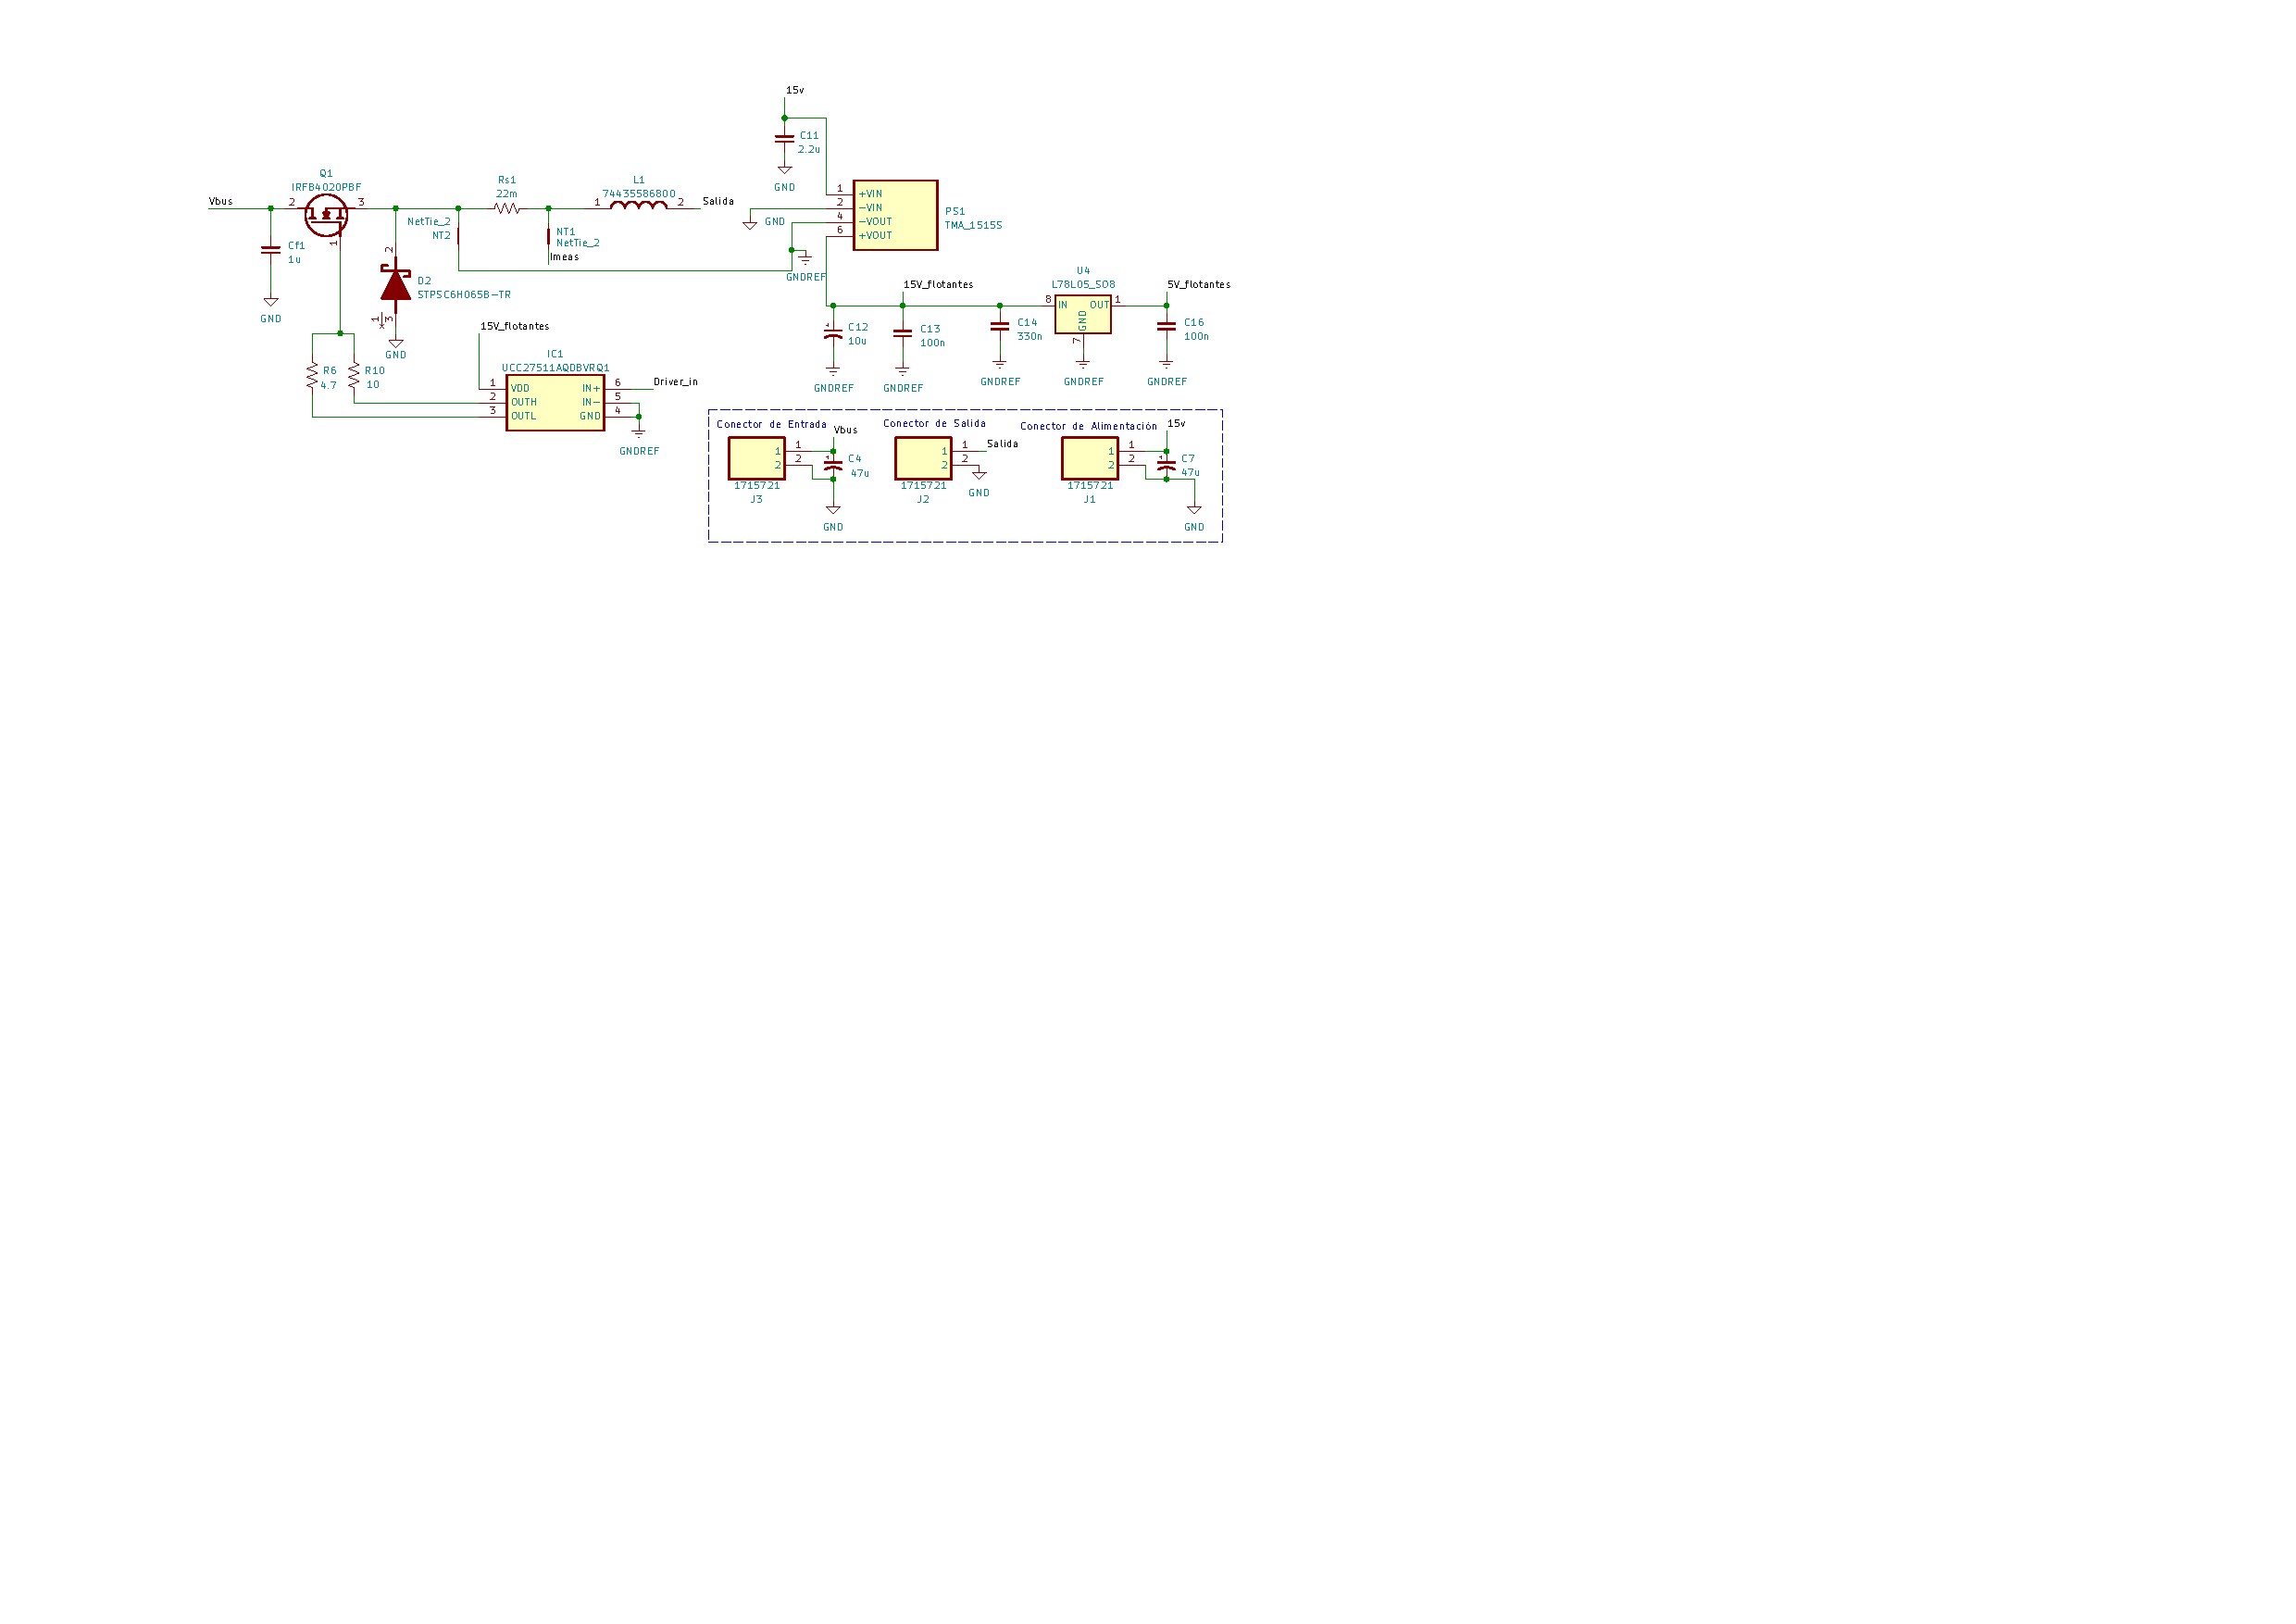
\includegraphics[width=1\textwidth]{PKicadSch.pdf}}
    \vspace{2mm}
    {\raggedleft \textbf{Fuente:} Elaboración propia a partir del diseño esquemático realizado en KiCad. \par}
\end{figure}

\subsubsection{Bloque de acondicionamiento de corriente}
La conexión Kelvin es el punto desde el cual se obtiene la caída de tensión de la resistencia de medida proporcional a la corriente que fluye por ella. Esta señal $I_\text{meas}$ se amplifica ($G = - 25\text{ V/V}$) a través de la red de resistencias de los operacionales (U2) que se aprecia en la Figura \ref{fig:Acondicionamiento_Kicad}. 

Con el objetivo de obtener estabilidad en el lazo de control y filtrar el ruido de alta frecuencia producido por la conmutación del N-MOS se emplean 3 filtros paso bajo en cascada.
\begin{itemize}
    \item \textbf{Filtro de entrada:} el filtro formado por $R_1$ y $C_1$ atenua los transitorios bruscos de alta frecuencia de la señal de la resistencia de medida, protegiendo el integrado con un coste en el comportamiento dinámico muy reducido.  
    \item \textbf{Filtro de la primera etapa:} el filtro formado por $R_5$ y $C_2$ introduce un polo a aproximadamente $1{,}36\,\text{MHz}$, acotando el ancho de banda y mejorando la estabilidad del OPAMP.
    \item \textbf{Filtro de la segunda etapa:} el filtro formado por $R_{11}$ y $C_5$ introduce un polo a aproximadamente $2{,}08\,\text{MHz}$, atenuando más la señal de la primera etapa y librando a la señal de ruido de alta frecuencia. 
\end{itemize} 

La señal de salida ($I_\text{sense2}$), representa la corriente instantánea a través del bus de forma amplificada y libre de ruido. 

\begin{figure}[H]
    \centering
    \fontsize{10}{12}\selectfont 
    \ffigbox[\FBwidth]
    {   \caption[Esquema en KiCad de la etapa de acondicionamiento ]{Implementación en KiCad de la etapa de acondicionamiento con los componentes reales seleccionados para el montaje de la PCB.}
        \label{fig:Acondicionamiento_Kicad}}
    {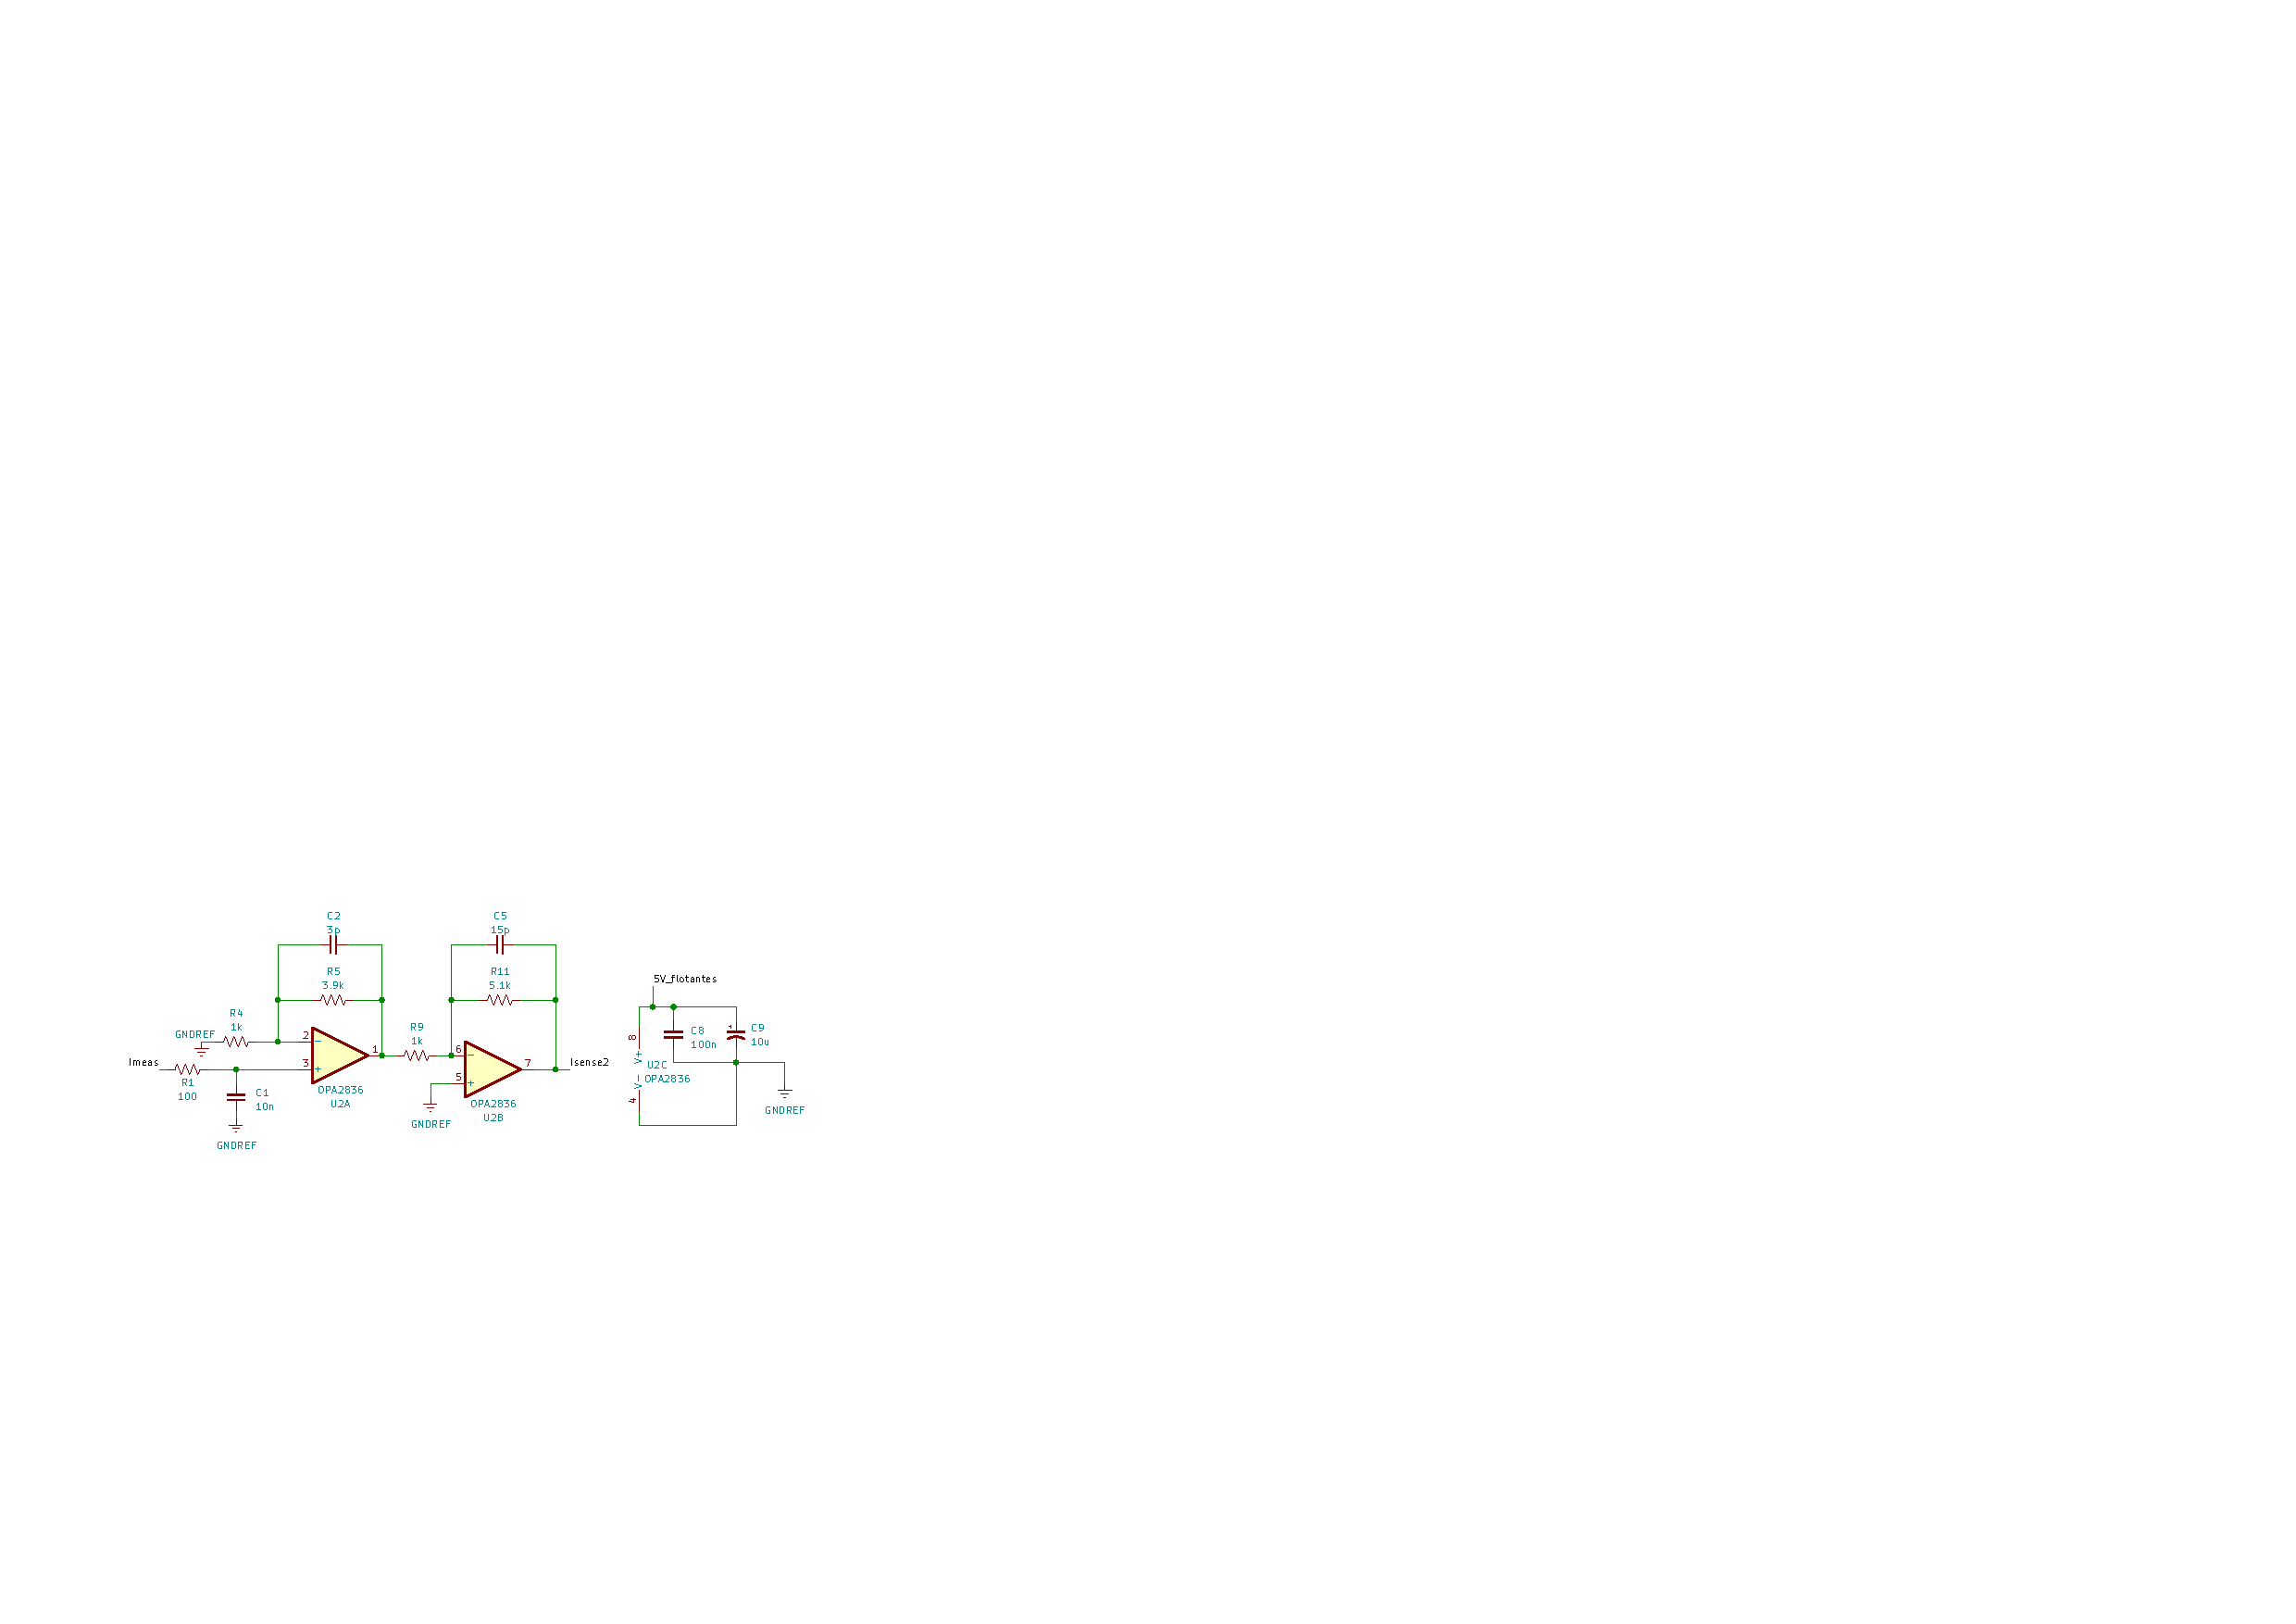
\includegraphics[width=1\textwidth]{AcondicionamientoKicadSch.pdf}}
    \vspace{2mm}
    {\raggedleft \textbf{Fuente:} Elaboración propia a partir del diseño esquemático realizado en KiCad. \par}
\end{figure}

\subsubsection{Bloque del lazo de histéresis y enclavamiento}

La conmutación se realiza mediante el uso de dos comparadores que establecen el estado de un biestable como se puede observar en la Figura \ref{fig:HisteresisKicad}. Para la comparación se establecen en los límites superior e inferior de la banda de histéresis ($I_\text{sup}$ e $I_\text{inf}$) el voltaje medible en la $R_\text{shunt}$ para el paso de la corriente definida, multiplicando el valor por la ganancia de acondicionamiento. De esta manera, las resistencias $R_{14}$, $R_{15}$, $R_{16}$ y $R_{17}$ establecen sendos divisores resistivos para obtener un valor intermedio de voltaje a partir de los 5 voltios flotantes el cual se ajusta a los límites deseados mediante los potenciómetros RV1 y RV2. 

La comparación de la señal amplificada frente a los umbrales se realiza mediante el LM319 (U3A y U3B), el cual por tener salida en colector abierto requiere de las resistencias $R_\text{18}$ y $R_\text{19}$ para la transición entre el nivel bajo y el nivel alto que llega al SN74LVC2G02DCUR (IC2). Las puertas NOR se enrutan de modo que se configuren como biestable RS, memorizando el estado del limitador y teniendo como salida la señal Q. Esta es, junto a la salida del temporizador (la cual es normalmente 1), una de las entradas de la puerta \textit{AND} encargada de activar y desactivar el \textit{driver} que alimenta al transistor. 

\begin{figure}[H]
    \centering
    \fontsize{10}{12}\selectfont 
    \ffigbox[\FBwidth]
    {   \caption[Esquema en KiCad del lazo de histéresis y enclavamiento]{Implementación en KiCad del lazo de histéresis y control con los componentes reales seleccionados para el diseño físico de la PCB}
        \label{fig:HisteresisKicad}}
    {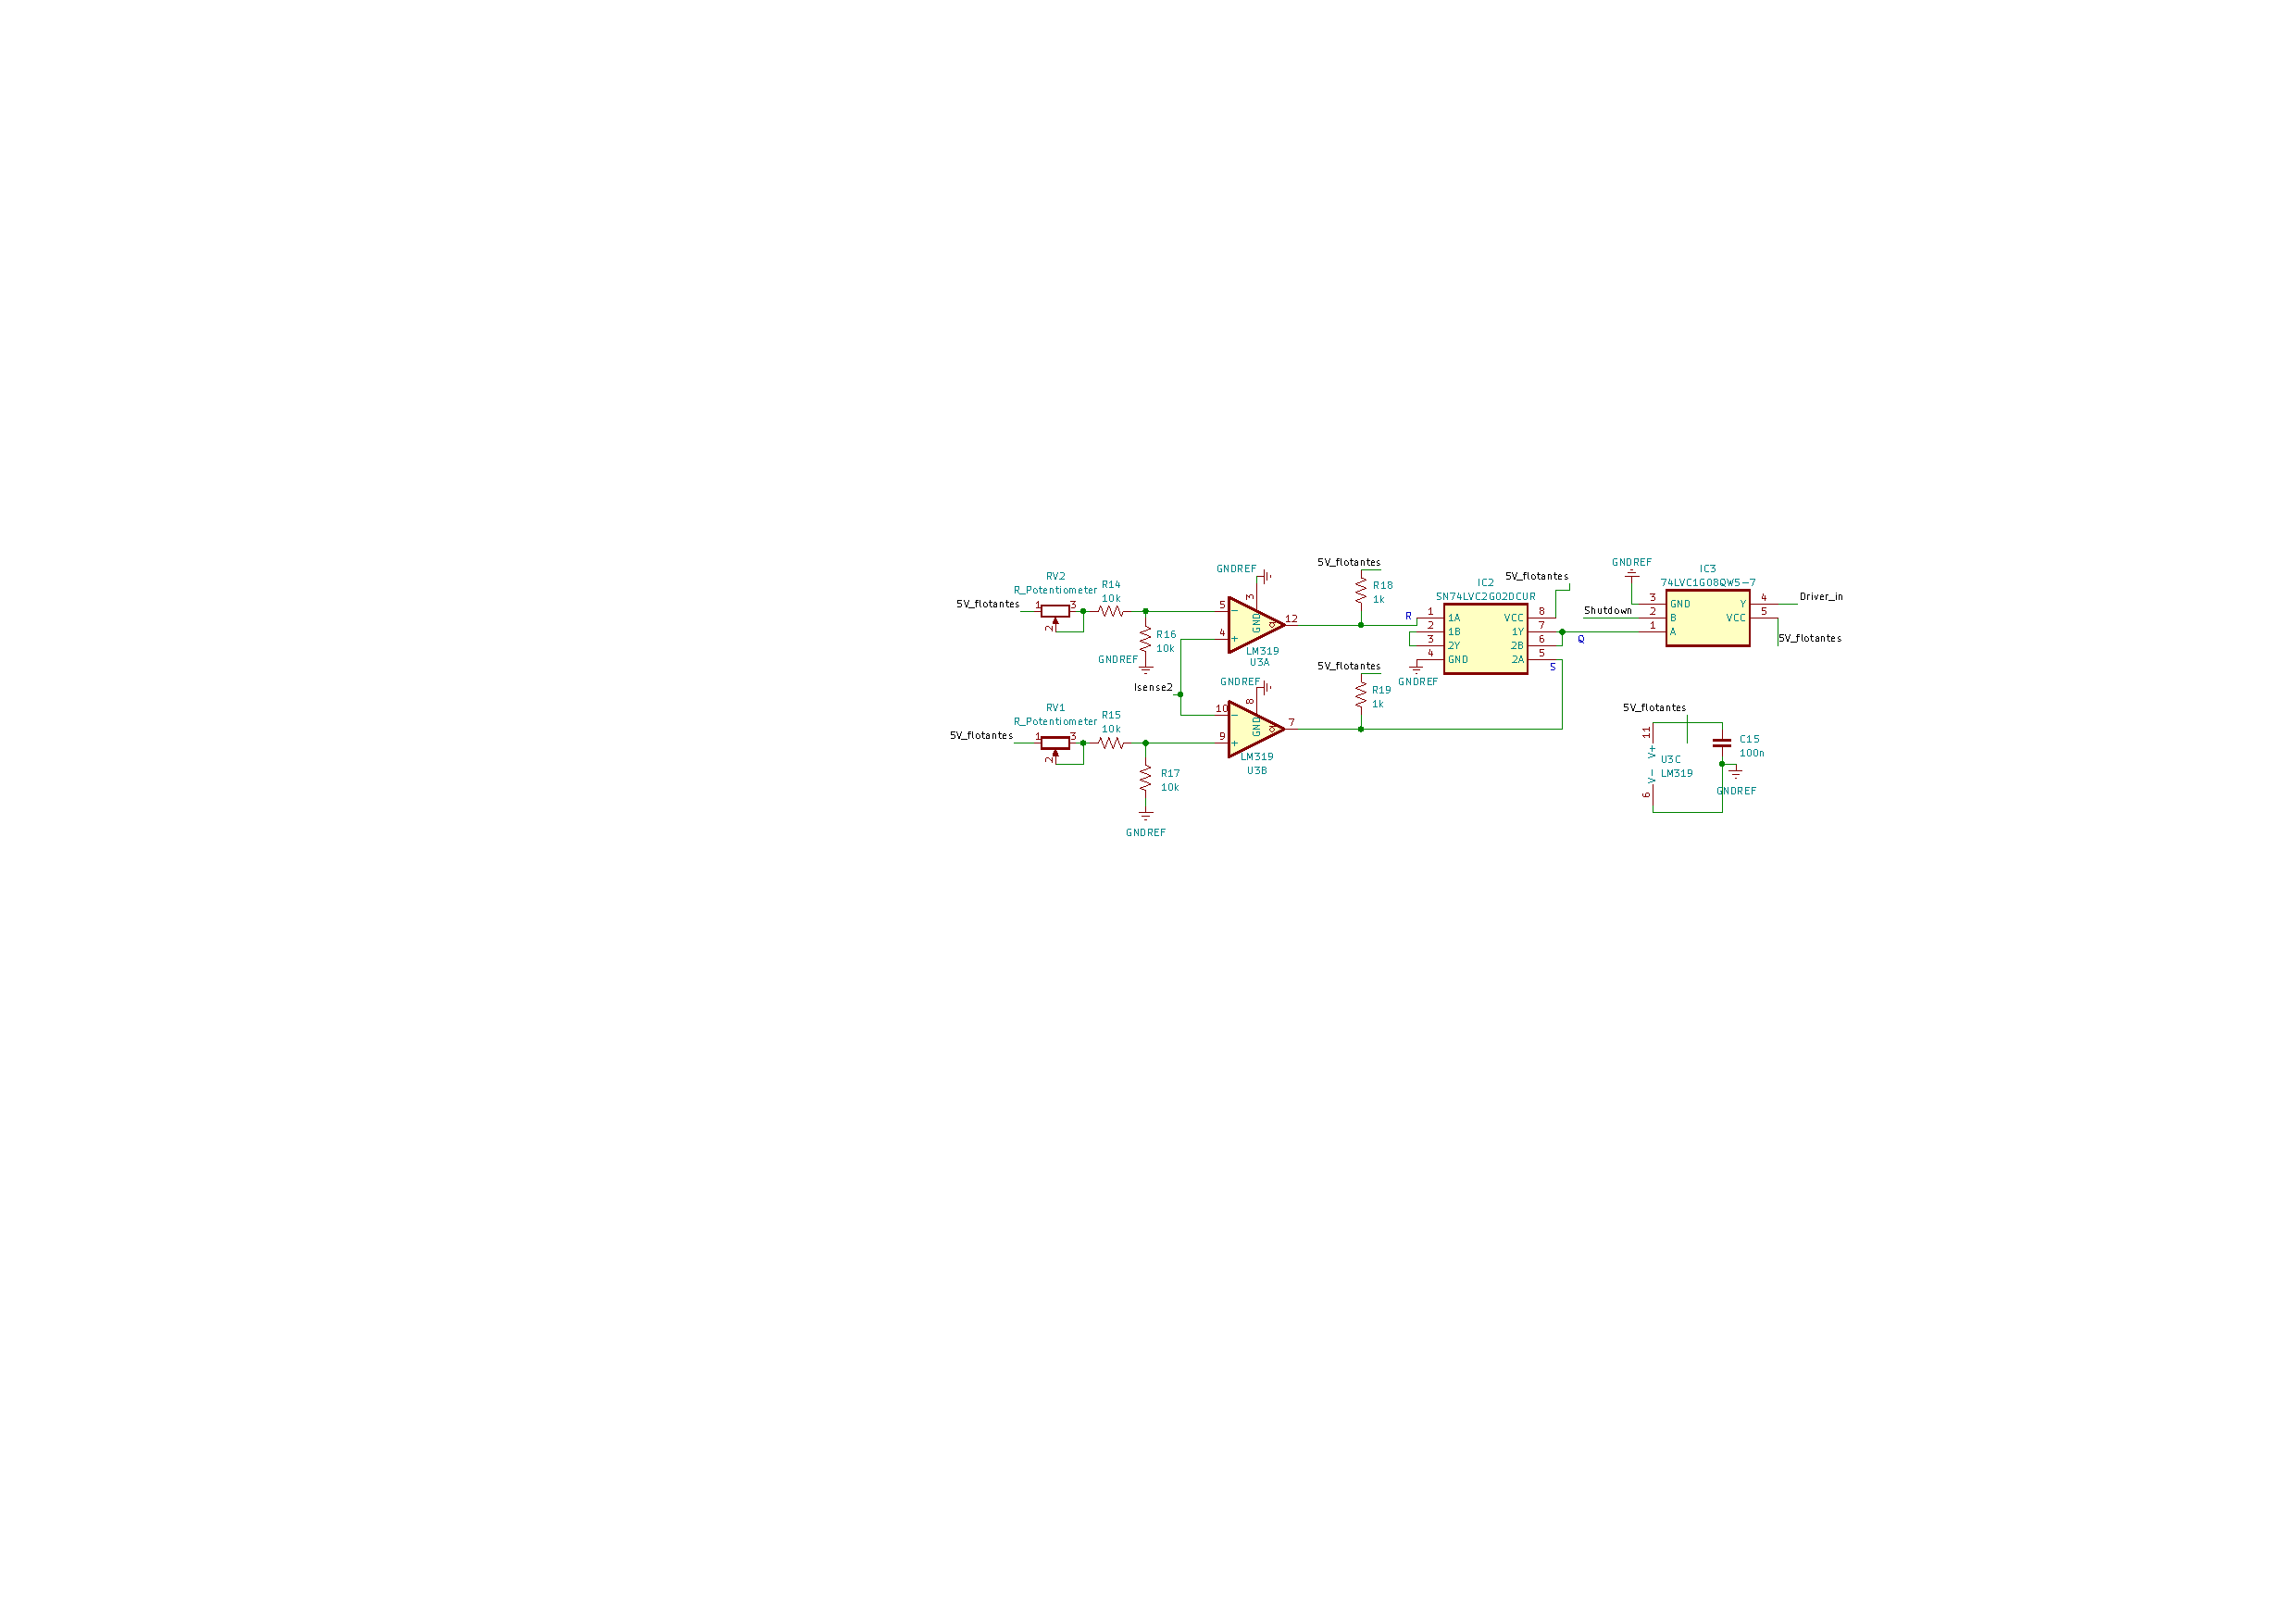
\includegraphics[width=1\textwidth]{HisteresisKicadSch.pdf}}
    \vspace{2mm}
    {\raggedleft \textbf{Fuente:} Elaboración propia a partir del diseño esquemático realizado en KiCad. \par}
\end{figure}

\subsubsection{Bloque de temporización}
La última etapa principal, el temporizador de la Figura \ref{fig:Temporizador_Kicad}, se encarga de contabilizar la duración de la sobrecorriente y, de sobrepasar el limite establecido, enviar la orden que provoca el enclavamiento. 

La monitorización se realiza mediante dos comparadores LM393 (U1) en cascada con dos propositos diferenciados. 
El integrado U1A compara la caída de voltaje en la resistencia de medida tras su amplificación ($Isense2$) con una referencia de voltaje realizada mediante el divisor formado por $R_2$ y $R_3$, y la raíl flotante de 5 voltios. De esta manera se obtiene un voltaje proporcional a la caída de voltaje provocada por un paso de $3{,}7\,A$.

Una vez se mide un voltaje mayor al límite establecido, el condensador se empiza a cargar a través de la resistencia $R_7$ y el paso por el ánodo del diodo D3. Para fallos menores al tiempo de \textit{trip-off}, el condensador se descarga a través de la resistencia de mayor valor $R_8$ y el mismo diodo, dotando al sistema de memoria térmica.

La red RC ($R_7$ y $Ct_1$) se adapta para que el paso de $1{,}5$ ms equivala al establecido con el divisor resistivo, evitando el uso innecesario de resistencias extras. En caso de superar el tiempo de \textit{trip-off}, el voltaje almacenado en el condensador será mayor que el establecido mediante las $R_2$ y $R_3$ cambiando el nivel de salida del comparador,el cual en caso nominal es alto, a nivel bajo. El cambio de la señal provoca que haya un 0 lógico a la entrada de la puerta \textit{AND} y, por tanto, el MOSFET queda abierto y el fallo extinguido. 
\begin{figure}[H]
    \centering
    \fontsize{10}{12}\selectfont 
    \ffigbox[\FBwidth]
    {   \caption[Esquema en KiCad de la etapa de temporización]{Implementación en KiCad del temporizador asimétrico de protección contra sobrecorrientes con los componentes reales seleccionados para el diseño físico de la PCB.}
        \label{fig:Temporizador_Kicad}}
    {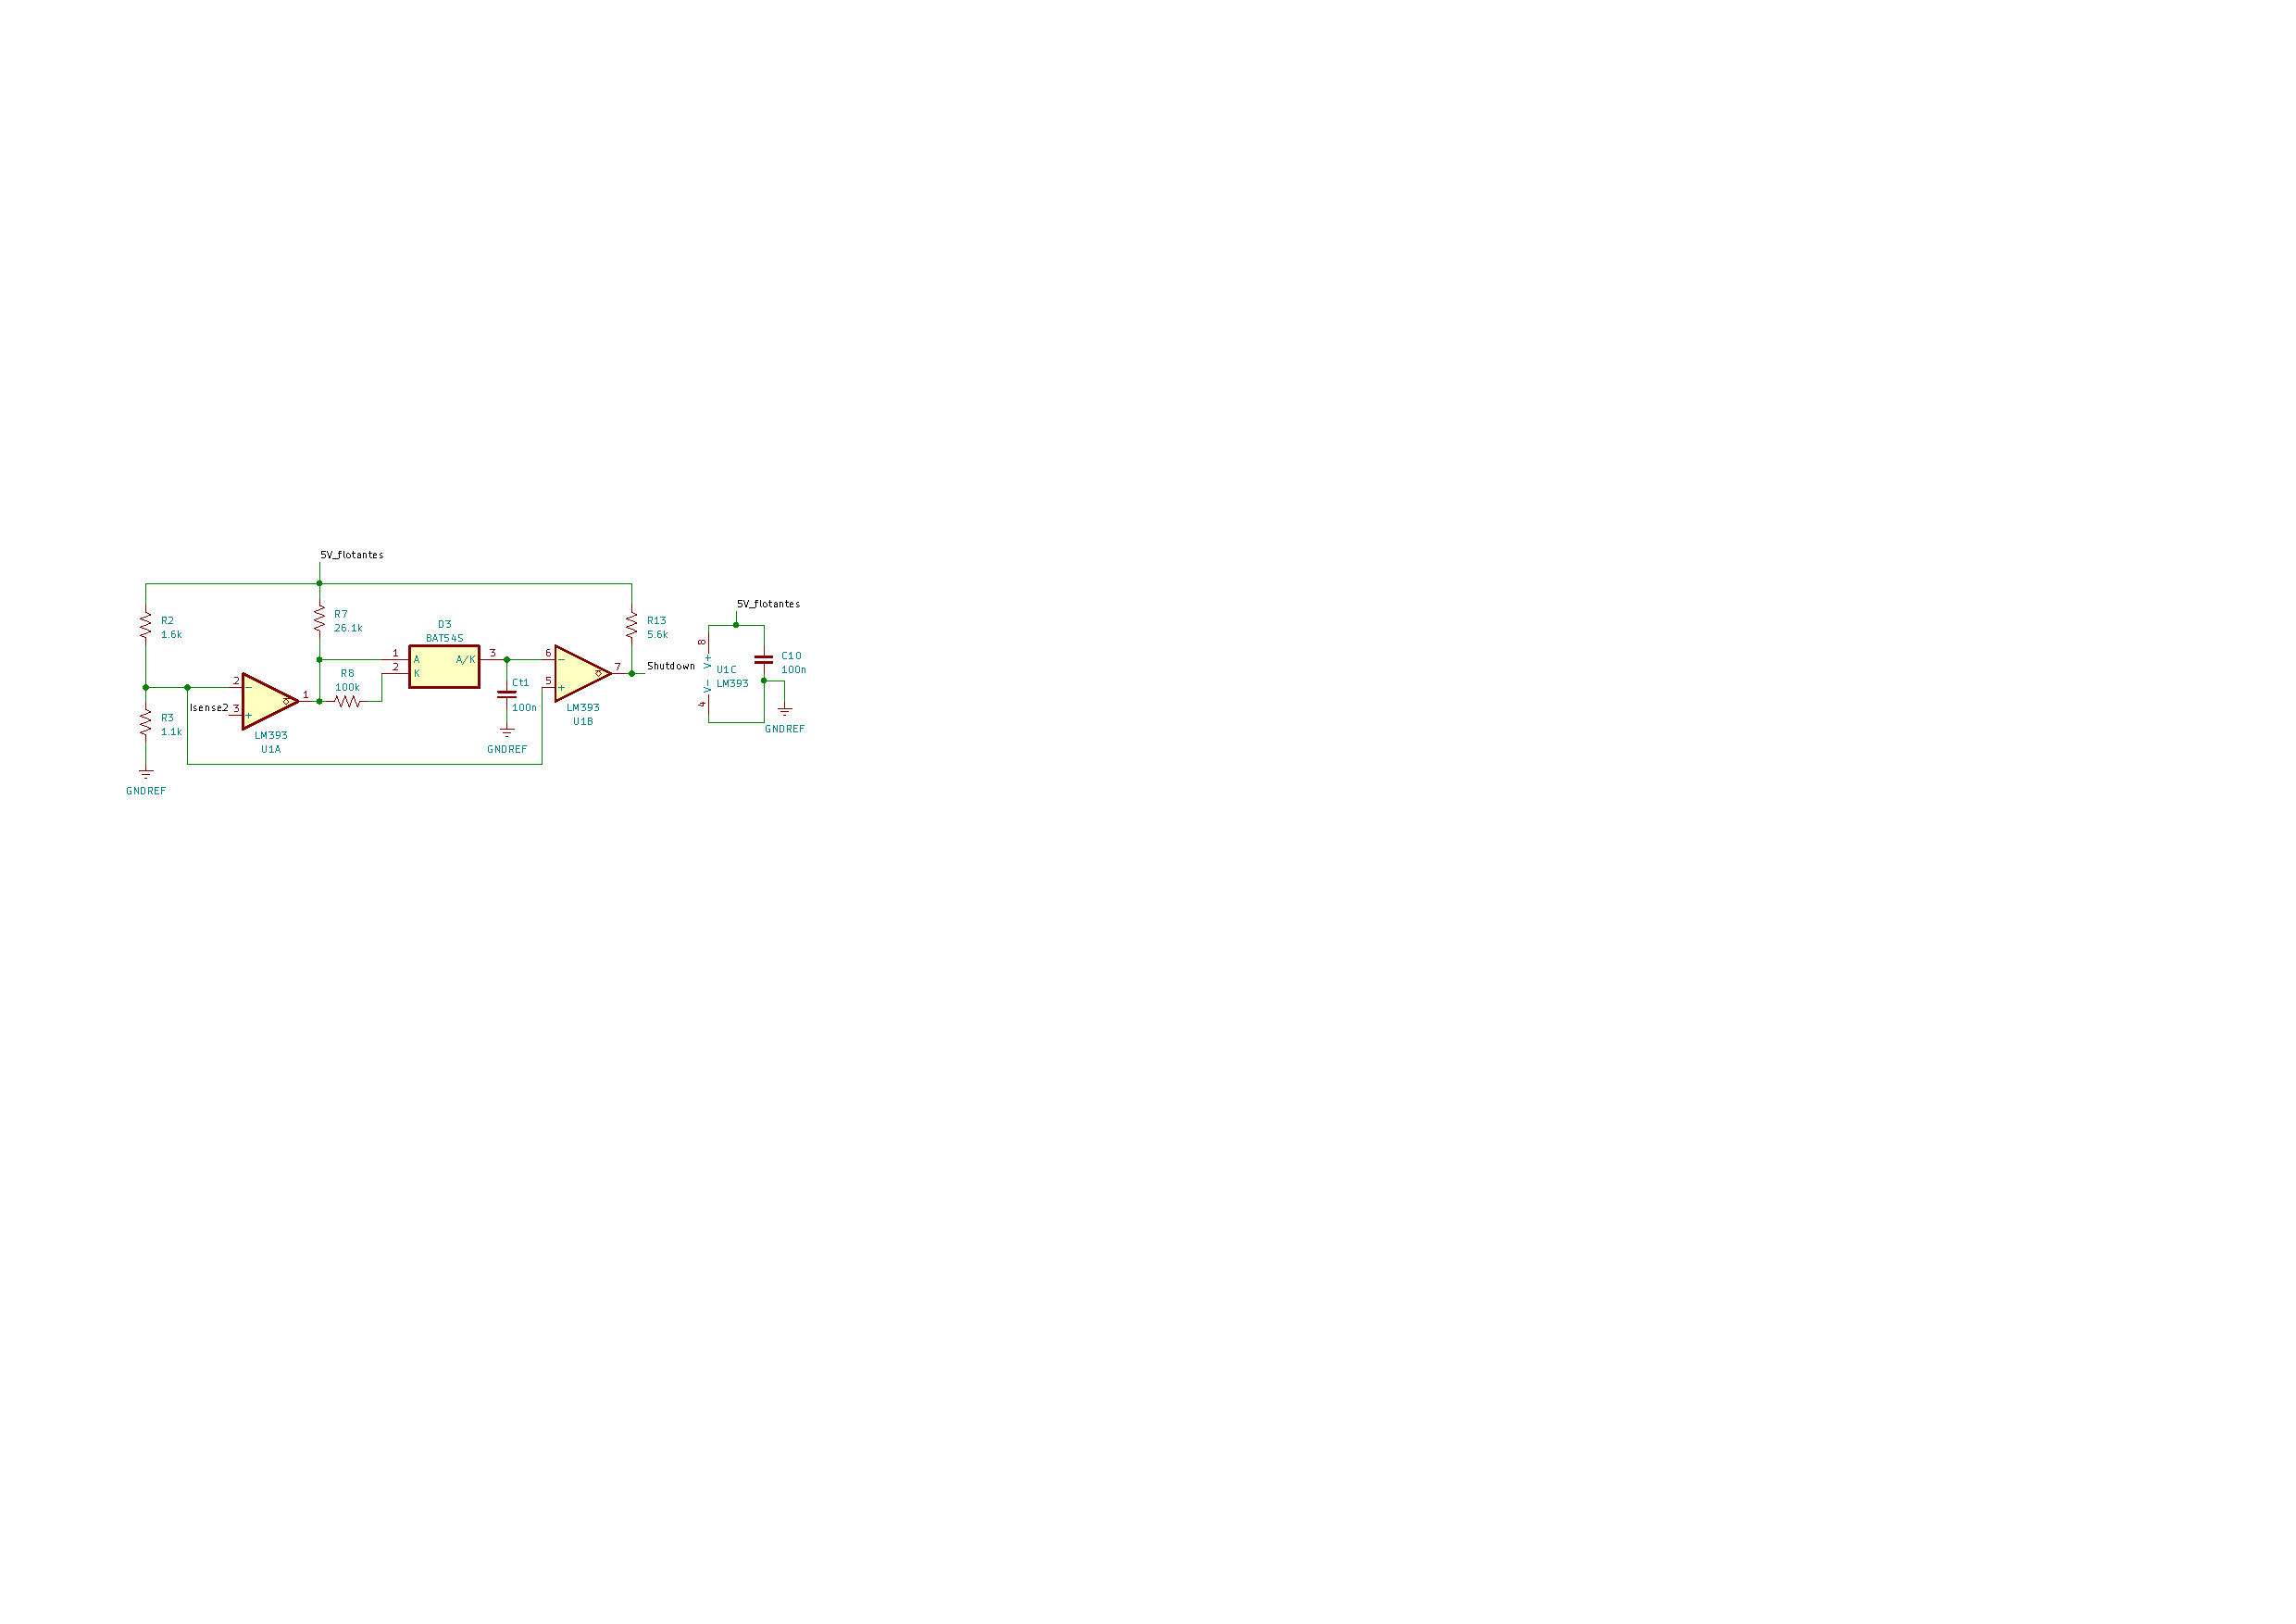
\includegraphics[width=1\textwidth]{TemporizadorKicadSch.pdf}}
    \vspace{2mm}
    {\raggedleft \textbf{Fuente:} Elaboración propia a partir del diseño esquemático realizado en KiCad. \par}
\end{figure}

\subsection{Modelado equivalente en PSIM e integración de efectos parásitos}
Una vez definido el esquema del circuito real en KiCad, el siguiente paso en el análisis es trasladar la arquitectura al entorno de simulación PSIM para validar el comportamiento del sistema. Sin embargo, para obtener resultados realistas que coincidan con el comportamiento del prototipo físico, el modelo no puede ser ideal por las limitaciones que nos impone la herramienta. Es por ello por lo que se emplea un modelo de comportamiento equivalente distribuido en los 3 bloques principales, integrando los tiempos de ptopagación de los integrados, las características parásitas de los componentes y elementos para la emulación de fallos. 

\subsubsection{Etapa de potencia, lógica de histéresis y bloques de retardo}
El núcleo de potencia y el lazo de histéresis se ven implementados en el modelo conductual de la Figura \ref{fig:Principal_psim}. El bus se alimenta con una fuente continua de $100\,\text{V}$ ($V_{bus}$) con dos condensadores no ideales en paralelo, el cerámico de ($C_{bus\_ceramico} = 1\,\mu\text{F}$) y el electrolítico ($C_{bus\_electrolitico} = 47\,\mu\text{F}$). Debido a limitaciones al introducir el modelo del \textit{driver} UCC27511A en PSIM, se ha empleado una fuente de tensión dependiente controlada por la señal de salida del lazo de control (salida de la puerta \textit{AND}) y una resistencia de puerta para excitar la capacidad parásita de la puerta del IRFB4020PBF, transistor modelado con las características de su hoja de datos. 

La comprobación de la capacidad de protección del circuito se realiza mediante dos resistencias en paralelo. Durante la operación nominal, el convertidor alimenta una resistencia de $R_{load1} = 40\,\Omega$ supliéndola con aproximadamente $2{,}5 A$. Para comprobar el estado de sobrecorriente, la resistencia en paralelo $R_{sc}$ de $0{,}1\,\Omega$ se conecta a tierra mediante el interruptor controlado por voltaje, provocando una resistencia de carga equivalente muy inferior a la nominal e induciendo una corriente masiva a través de la resistencia \textit{shunt}.

En cuanto al lazo de histéresis, se ha tenido especial atención a la respuesta temporal mediante la inclusión de bloques de retrasos equivalentes a los tiempos de los componentes elegidos. Por no ser en la electrónica real instantánea la conmutación, se han incluido los siguientes bloques: 
\begin{itemize}
    \item \textbf{Comparador LM319:} bloques de $80\,\text{ns}$. 
    \item \textbf{Puertas lógicas 74LVC:} bloques de $10\,\text{ns}$ para el tiempo combinado de ambas puertas.
    \item \textbf{\textit{Driver} UCC27511A:} bloque de $23\,\text{ns}$.
\end{itemize}
La inclusión en la simulación de estos $113\,\text{ns}$ de retraso permiten realizar un ajuste de los límites de histéresis más adecuado ya que, por este retraso entre medida y cambio de estado del transistor, los límites $I_\text{sup,PCB}$ e $I_\text{inf,PCB}$ deben ser inferior y superior respectivamente a los teóricos buscados ($I_\text{sup} = 4{,}5\,A$ e $I_\text{inf} = 3{,}7\,A$).
Dentro de la Figura \ref{fig:Principal_psim}, se emplean las características de la hoja de datos para el diodo, el inductor, los condensadores, el MOSFET, los comparadores LM319 y las puertas lógicas, además de la respuesta temporal del \textit{driver}.
\begin{figure}[H]
    \centering
    \fontsize{10}{12}\selectfont 
    \ffigbox[\FBwidth]
    {   \caption{Esquema de la etapa de potencia y del control por histéresis del limitador de corriente conmutado implementado en PSIM}
        \label{fig:Principal_psim}}
    {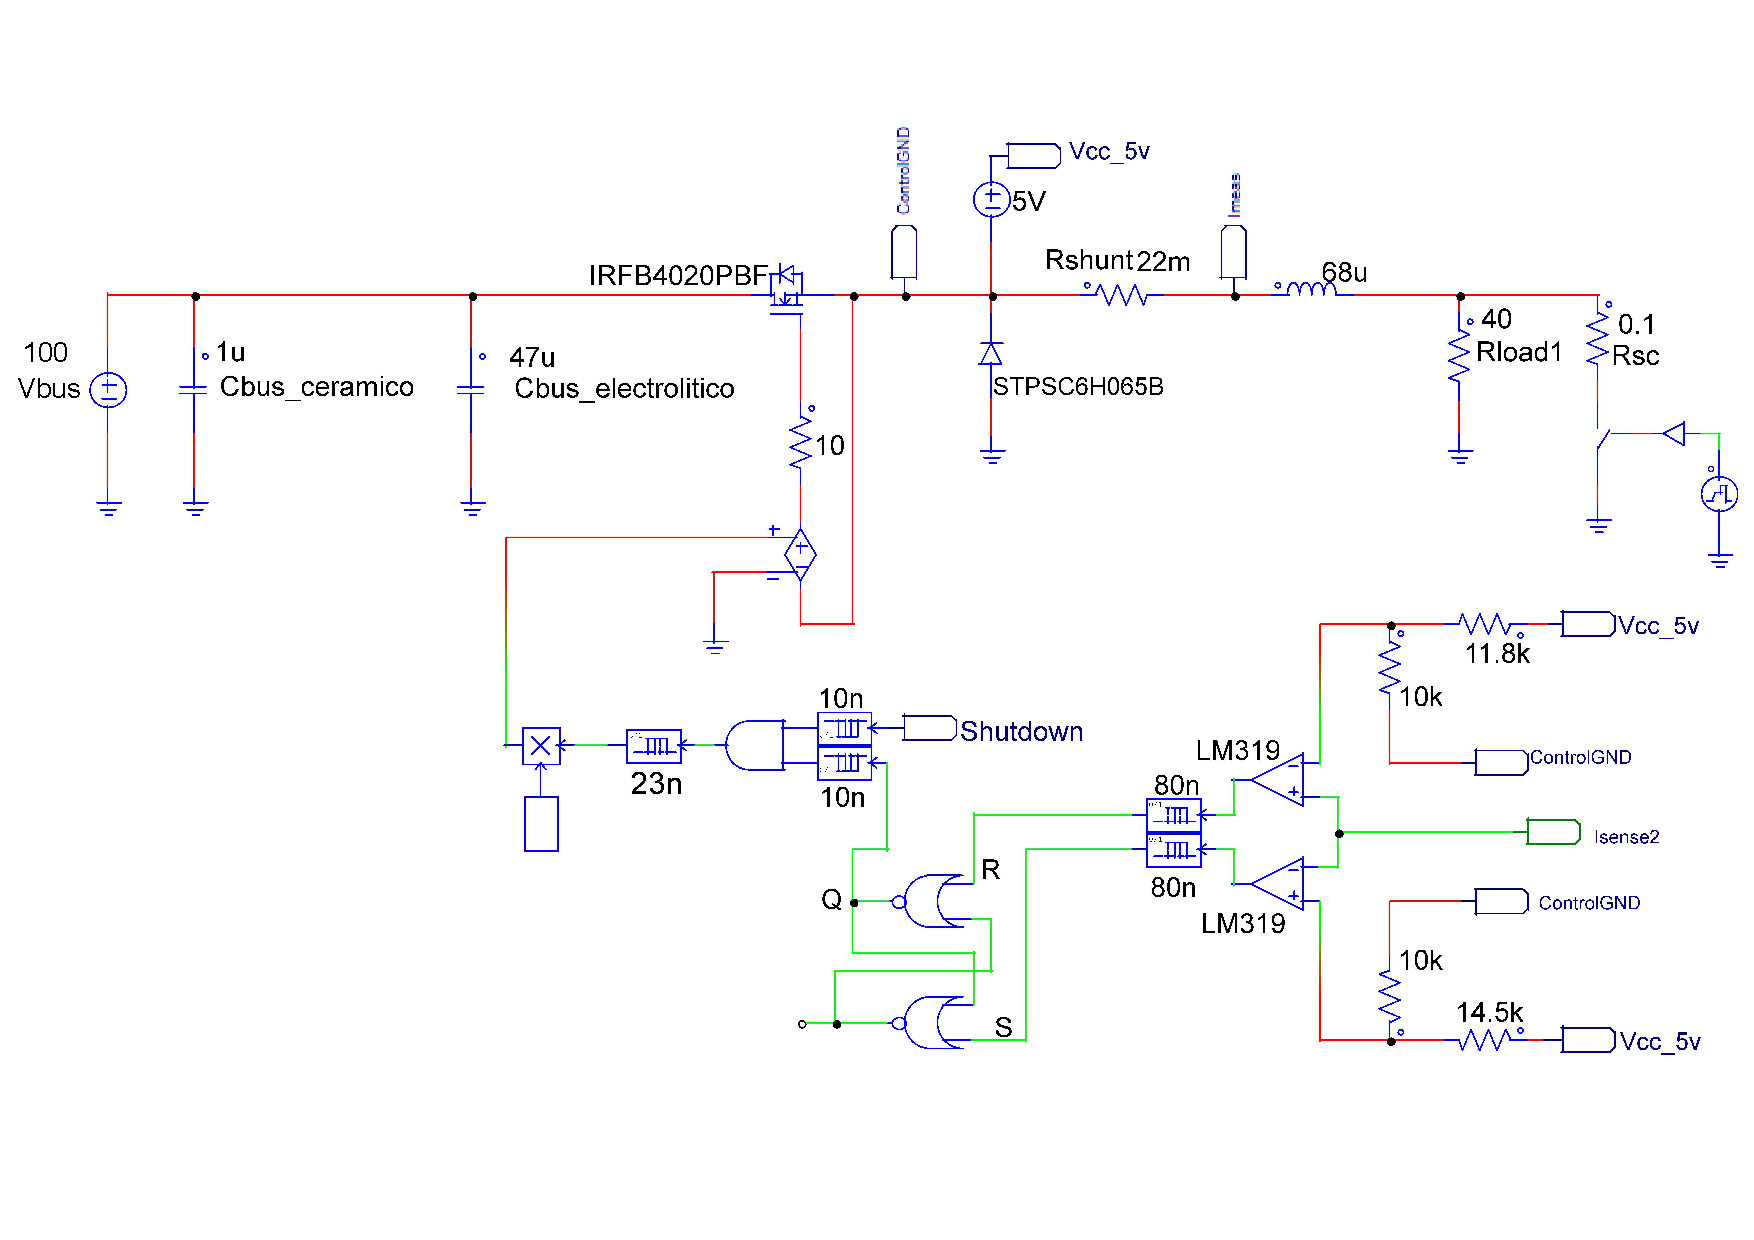
\includegraphics[width=0.9\textwidth]{Principal_psim.pdf}}
    \vspace{2mm}
    {\raggedleft \textbf{Fuente:} Elaboración propia a partir del diseño esquemático realizado en PSIM. \par}
\end{figure}

\subsubsection{Bloque de acondicionamiento de señal}
La etapa de acondicionamiento analógico en PSIM (Figura \ref{fig:Acondicionamiento_psim}) replica de forma directa la topología en cascada diseñada en KiCad, garantizando así una correspondencia exacta en ganancia y respuesta en frecuencia entre el circuito simulado y el hardware. Las características parásitas se emplean en el OPA2836 con el objetivo de obtener un resultado aproximado a la realidad y el filtro pasivo de entrada se omite debido a que, en la herramienta de simulación, el acoplamiento electromagnético debido a las señales de alta frecuencia no afecta a otros componentes. 
\begin{figure}[H]
    \centering
    \fontsize{10}{12}\selectfont 
    \ffigbox[\FBwidth]
    {   \caption[Circuito de acondicionamiento de corriente implementado en PSIM]{Etapa de acondicionamiento analógico de la caída de tensión en $R_\text{shunt}$, implementada mediante amplificadores operacionales ADA4807.}
        \label{fig:Acondicionamiento_psim}}
    {\includegraphics[width=1\textwidth]{Acondicionamiento_psim.pdf}}
    \vspace{2mm}
    {\raggedleft \textbf{Fuente:} Elaboración propia a partir del diseño esquemático realizado en PSIM. \par}
\end{figure}

\subsubsection{Emulación de colector abierto y lazo de enclavamiento del temporizador}
El circuito de temporización se ha modelado en PSIM según la arquitectura detallada en la Figura \ref{fig:Timer_psim} teniendo en cuenta las restricciones de los comparadores en PSIM. Por ser el LM393 un componente con salida en colector abierto, este comportamiento se emula mediante el empleo de un interruptor controlado por la tensión de salida de un comparador. Al cambiar el valor del comparador, la resistencia de \textit{pull-up} queda conectada a la masa de control, permitiendo la carga a través de esta resistencia y el raíl de alimentación de $5\,\text{V}$.

Cuando la señal de corriente se encuentra por debajo del límite establecido, el interruptor está abierto impidiendo la carga del condensador. Una vez la corriente es suficiente, el valor del comparador cambia cerrando el interruptor y conectando la resistencia a tierra, y en este instante comienza la carga a través del diodo (valores de la hoja de datos del BAT54). En caso de no mantenerse la sobrecorriente, el BJT que actúa como interruptor satura y deriva la tensión de control a masa, descargando el condensador a través de la resistencia de descarga. 

El mayor cambio respecto a la implementación real es el enclavamiento. Debido a ser dependientes entre si \textit{Shutdown} y $V_\text{th,tiempo}$, al apagarse el MOSFET y descargarse el condensador, el valor \textit{Shutdown} vuelve a su valor inicial (normalmente '1') y se entra enun bucle que no permite ni enfriarse al MOSFET ni el enclavamiento. Para solventar este problema se opta por forzar el enclavamiento en el momento del cambio de valor de la señal \textit{Shutdown}. Un interruptor controlado por el voltaje invertido de la salida se encuentra entre el valor de referencia y la masa de control, estando normalmente la masa aislada y siendo el valor en $V+$ el establecido por el divisor resistivo. En el instante de activación de la protección, la señal en el interruptor cambia y se conecta $V+$ a tierra, estableciendo en él pin un valor de $0$ voltios.

El valor de 0 voltios en la entrada del comparador provoca que el enclavamiento se mantenga una vez se cumpla el tiempo establecido, imitando de esta manera el comportamiento del circuito real.  
\begin{figure}[H]
    \centering
    \fontsize{10}{12}\selectfont 
    \ffigbox[\FBwidth]
    {   \caption[Circuito del temporizador asimétrico implementado en PSIM]{Circuito del temporizador analógico con red RC asimétrica de carga y descarga, incluyendo la realimentación positiva para la modificación dinámica de la referencia.}
        \label{fig:Timer_psim}}
    {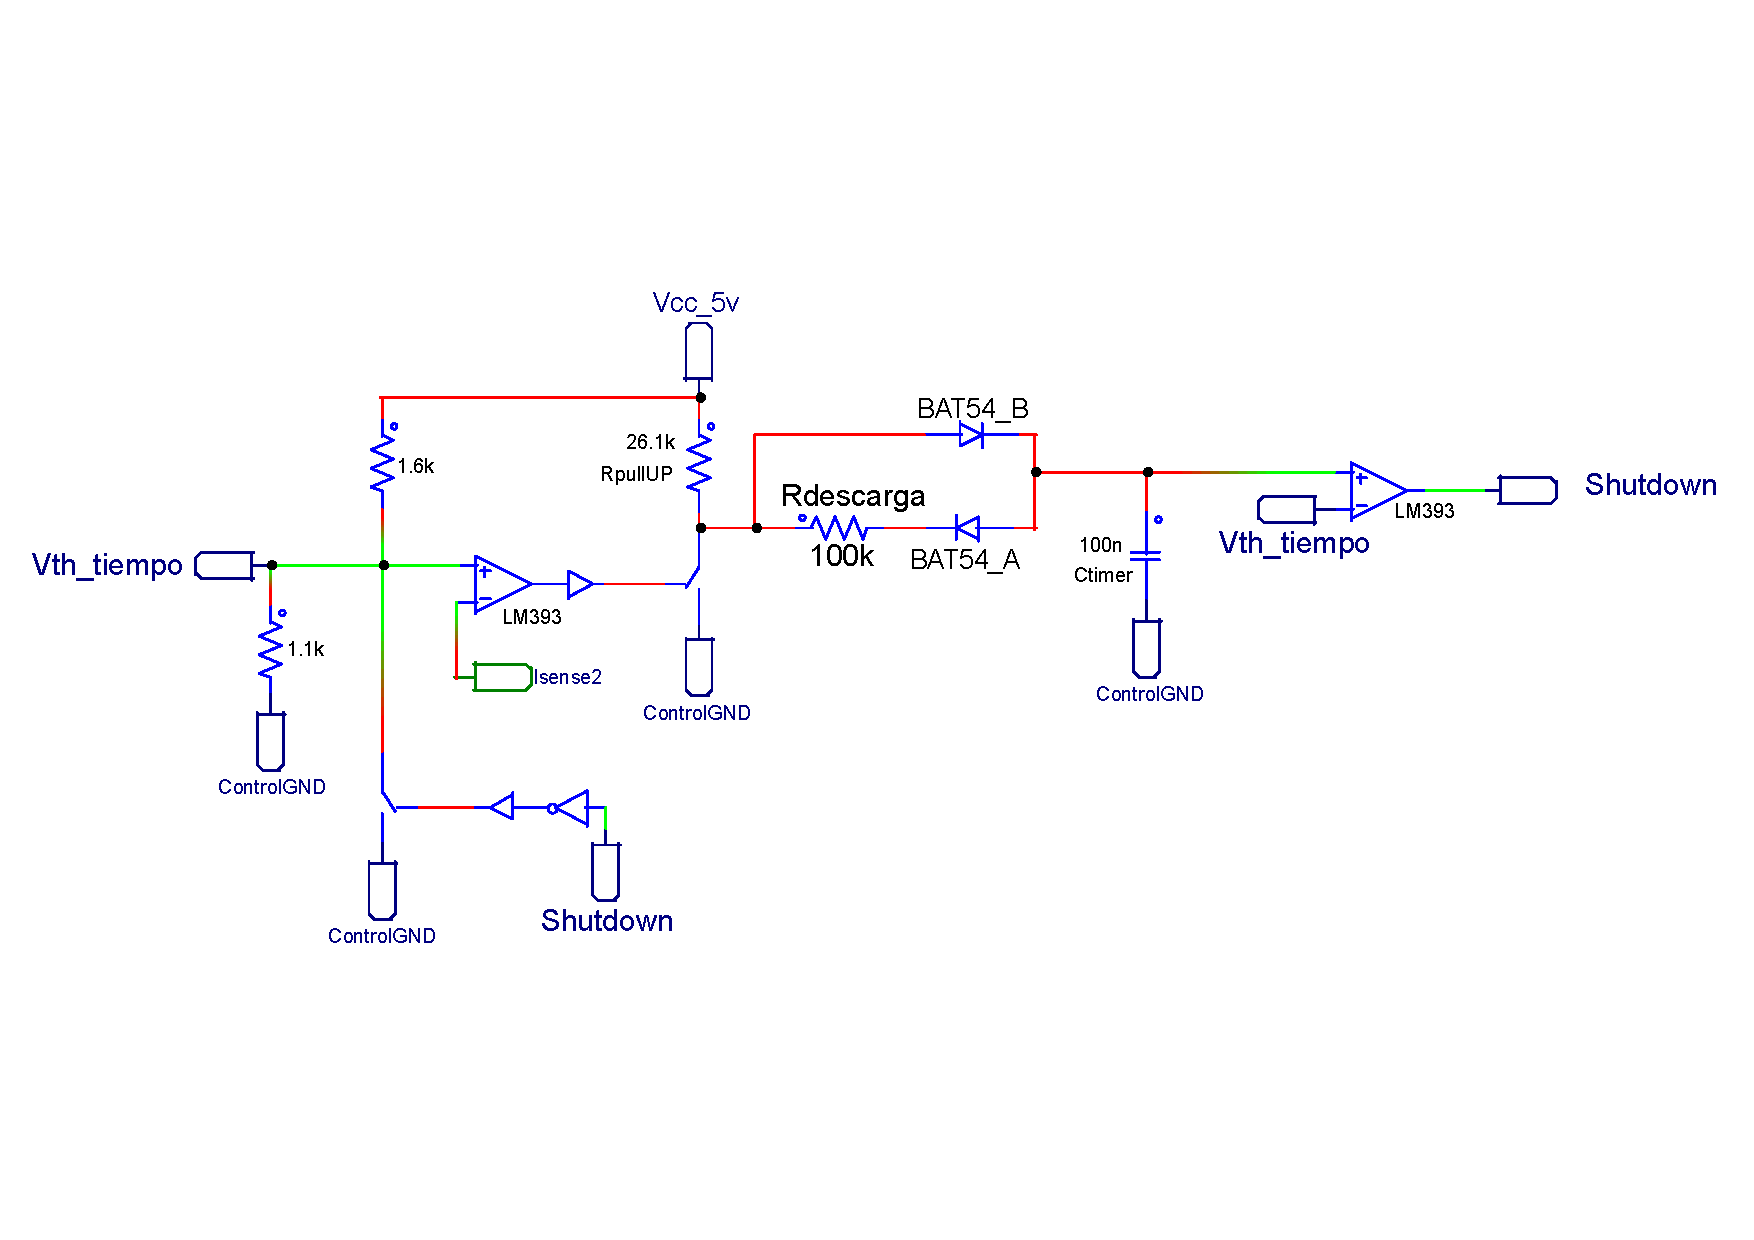
\includegraphics[width=1\textwidth]{Temporizador_PSIM.pdf}}
    \vspace{2mm}
    {\raggedleft \textbf{Fuente:} Elaboración propia a partir del diseño esquemático realizado en PSIM. \par}
\end{figure}


\subsection{Análisis dinámico y discusión de resultados de la simulación}
\label{subsec:analisis_dinamico}
A partir de los modelos presentados, se discuten a continuación los resultados de simulación obtenidos tras someter al LCL a diferentes fallos por sobrecorriente, tanto de forma transitoria como permanente. 
\subsubsection{Respuesta temporal ante cortocircuito permanente}
\label{subsubsec:corto_permanente}
La Figura~\ref{fig:Ishunt_fallo_permanente} muestra la corriente circulando por la resistencia de sensado $R_{\text{shunt}}$ al introducir un cortocircuito en el instante $t = 1~\text{ms}$. En condiciones nominales (sin fallo) el circuito suministra $2{,}5~\text{A}$ constantes a la carga hasta que se produce el suministro, realizado al conectar una resistencia paralela a la carga ($R_{\text{sc}} = 0{,}1~\Omega$).

Tras el cortocircuito, la corriente sufre un pico ascendente de corriente y el lazo de control detecta el cortocircuito, comenzando así tanto la carga del temporizador como el control del lazo de histéresis. La imagen muestra perfectamente los dos parámetros claves del LCL: el tiempo de limitación y los límites de histéresis. 

Por un lado, la simulación valida el funcionamiento en conmutación del limitador durante un intervalo de tiempo $\Delta t = 1{,}496~\text{ms}$, valor prácticamente idéntico al valor teórico de \textit{trip-off} fijado en las especificaciones en $1{,}5~\text{ms}$. Transcurrido este tiempo durante el cual el circuito conmuta, la señal \textit{Shutdown} cambia a valor bajo como se verá en la Figura \ref{fig:IvsVgsvsEntradasAND} más adelante, y se produce el enclavamiento impidiendo el paso de corriente por la resistencia. 

Por otro lado, la simulación también permite ver los límites de corriente entre los cuales actúa el limitador, siendo estos ($I_{\text{sup}} = 4{,}465~\text{A}$ e $I_{\text{inf}} = 3{,}708~\text{A}$) prácticamente idénticos a los límites teóricos del diseño ($4{,}5~\text{A}$ y $3{,}7~\text{A}$). La pequeña variación en los límites viene justificada por el retardo del lazo de control $t_{\text{sense}}$, lo cual provoca que los valores teóricos de las referencias de histéresis se tengan que adaptar para variar el estado del MOSFET de forma predictiva. Esto se puede ver por ejemplo en el límite superior de histéresis de la Figura \ref{fig:Principal_psim}, el cual corresponde a los $2{,}29~V$ debidos al paso de $4{,}16~A$ por la resistencia de medida. Una vez medido este valor, se da la orden de abrir el N-MOS y el retardo provoca que la transición se produzca al llegar la corriente a prácticamente los $4{,}5~\text{A}$ buscados. 

Por ultimo, los resultados demuestran el correcto dimensionamiento de la inductancia al ser esta capaz de limitar la corriente en la banda de histéresis sin permitir un \textit{overshoot} destructivos para el MOSFET. 
\begin{figure}[H]
    \centering
    \fontsize{10}{12}\selectfont 
    \ffigbox[\FBwidth]
    {   \caption[Simulación de respuesta temporal ante fallo permanente]{Respuesta dinámica de la corriente por $R_\text{shunt}$ ante un cortocircuito permanente, mostrando el tiempo de operación conmutada previa al enclavamiento.}
        \label{fig:Ishunt_fallo_permanente}}
    {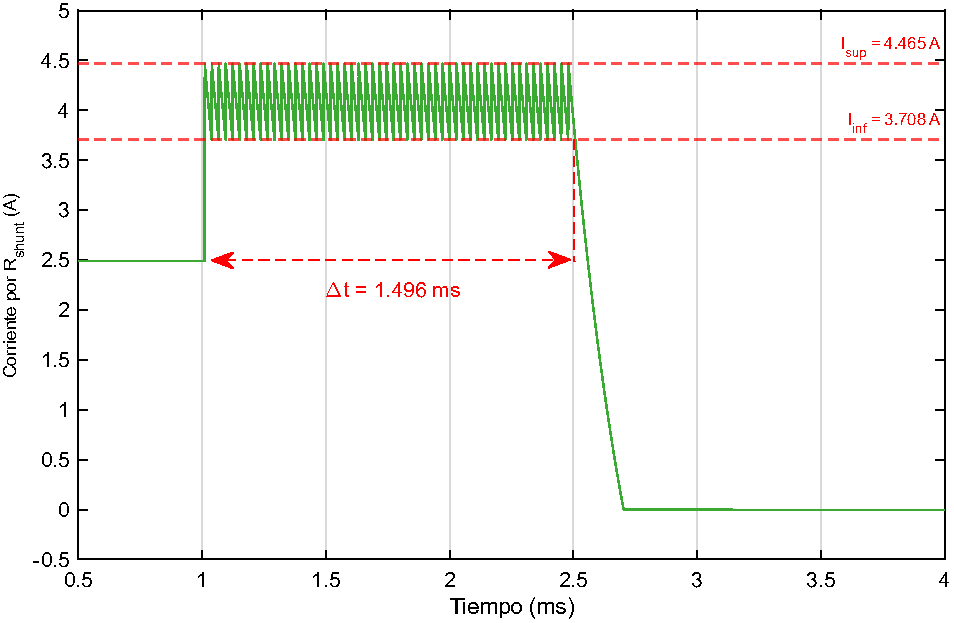
\includegraphics[width=1\textwidth]{Ishunt_fallo_permanente.pdf}}
    \vspace{2mm}
    {\raggedleft \textbf{Fuente:} Elaboración propia en MATLAB a partir de los resultados obtenidos en PSIM. \par}
\end{figure}


\subsubsection{Validación ante fallos sucesivos}
\label{subsubsec:memoria_termica}
Una vez vista la capacidad del limitador para proteger frente a un cortocircuito permanente, la Figura~\ref{fig:Ishunt_vs_Vctimer} muestra el comportamiento del circuito ante dos eventos cercanos en el tiempo. 

El primer fallo simula, por ejemplo, el encendido de un motor que provoca un pico de corriente de duración limitada. Durante el intervalo de la sobrecorriente, el condensador del temporizador se empieza a cargar a través de la resistencia de \textit{pull-up}, aumentando de esta manera el voltaje $V_{\text{Ctimer}}$ hasta aproximadamente  $1{,}6~\text{V}$. Una vez finaliza la sobrecorriente, la red RC asimétrica provoca que el condensador se descargue a través de la resistencia de descarga de alto valor, otorgando memoria térmica al sistema y asegurando un correcto enfriamiento del transistor. 

Debido a la red asimétrica, al provocarse el segundo cortocircuito en $t = 5{,}3~\text{ms}$ el condensador $C_{\text{timer}}$ no se ha descargado por completo (el transistor no se encuentra a temperatura nominal) y el voltaje que se mantiene el mismo será de entorno a $1{,}25~\text{V}$. Al empezar el cortocircuito antes de la descarga, el tiempo para que la tensión $V_{\text{Ctimer}}$ llegue al umbral de disparo ($V_{\text{th,tiempo}} = 2{,}035~\text{V}$ correspondiente a la carga del condensador durante $1{,}5~\text{ms}$) se reduce a $\Delta t = 1{,}081~\text{ms}$.

Los resultados obtenidos corresponden a lo modelado y muestran quela memoria térmica del sistema, reduciendo el tiempo de limitación en caso de fallos consecutivos para evitar sobrepasar la temperatura máxima del semiconductor.
\begin{figure}[H]
    \centering
    \fontsize{10}{12}\selectfont 
    \ffigbox[\FBwidth]
    {   \caption[Simulación de la dinámica de $V_\text{Ctimer}$ frente a fallos sucesivos]{Análisis dinámico de la corriente por $R_\text{shunt}$ y la tensión acumulada en el condensador del temporizador ($V_\text{Ctimer}$), validando el diseño asimétrico de carga del temporizador.}
        \label{fig:Ishunt_vs_Vctimer}}
    {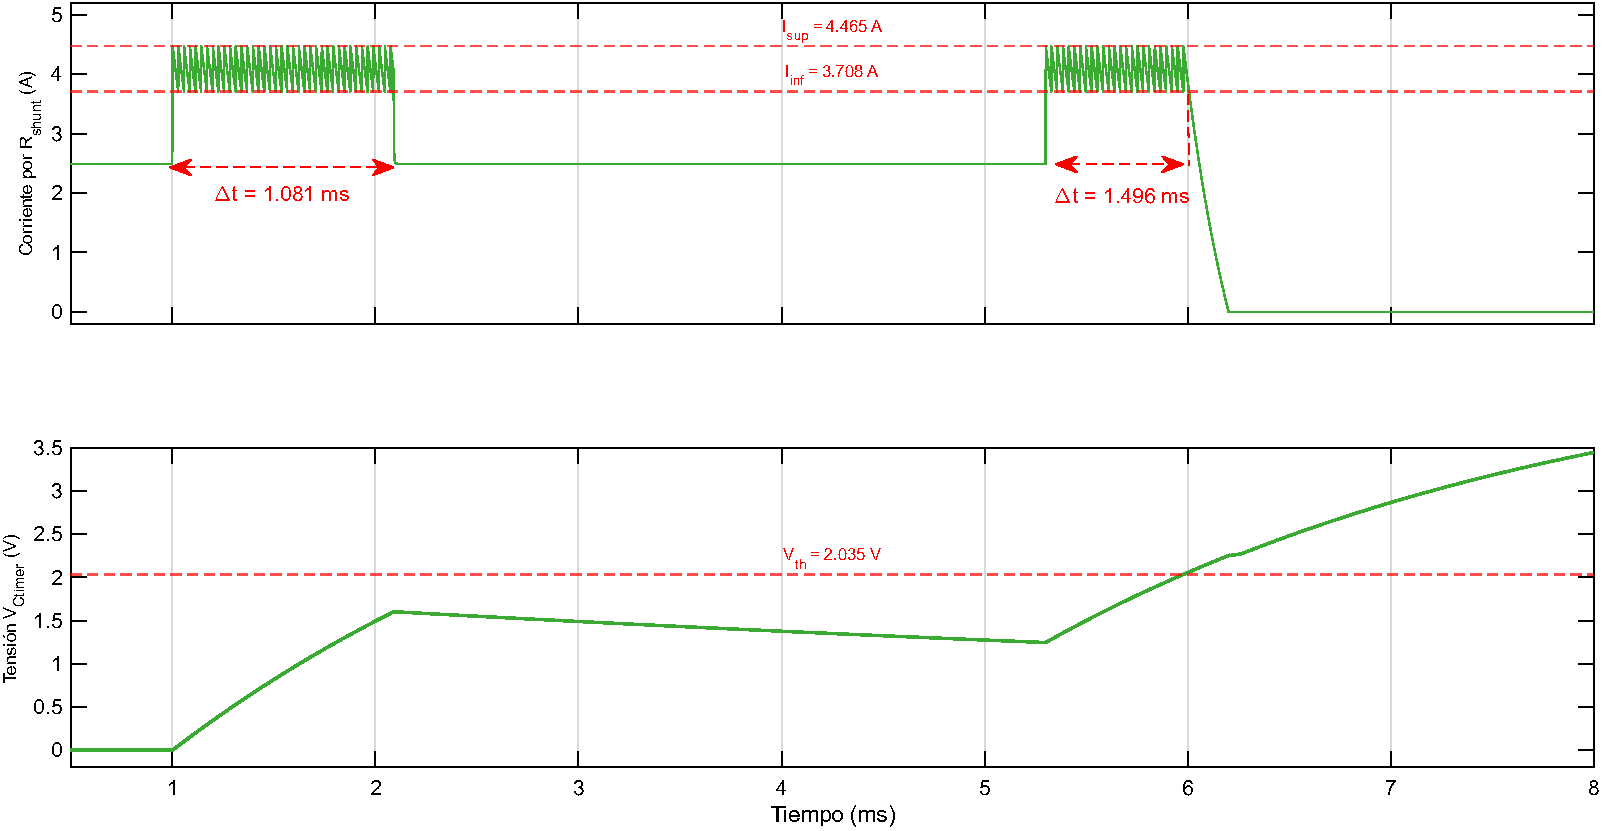
\includegraphics[width=1\textwidth]{IshuntvsVctimer.pdf}}
    \vspace{2mm}
    {\raggedleft \textbf{Fuente:} Elaboración propia en MATLAB a partir de los resultados obtenidos en PSIM. \par}
\end{figure}
\subsubsection{Caracterización del limitador mediante sobrecarga en rampa}
\label{subsubsec:caracterizacion_temporizador}
La Figura~\ref{fig:rampa_corriente} nos permite visualizar el valor de la corriente a partir del cual el circuito comienza a limitar la corriente de forma conmutada mediante el empleo de una fuente de corriente a modo de carga que incrementa de forma lineal la corriente drenada.

El circuito opera incialmente de forma nominal, suministrando a la carga una corriente continua de $2{,}5~\text{A}$. Una vez pasados $2~\text{ms}$ se conecta la fuente de corriente lineal creciente, aumentando de esta manera la corriente por la resistencia de sensado $R_{\text{shunt}}$. Como se puede comprobar en la gráfica, al alcanzar la corriente los $3{,}696~\text{A}$ (valor muy similar a los $3{,}7~\text{A}$ teóricos) se supera el umbral de activación de la referencia de entrada del primer comparador del temporizador, dando inicio a la carga del condensador $C_{\text{timer}}$ y activándose el limitador, validando así el diseño. 

La falta de rizado de conmutación propia del control por histéresis en la señal de corriente se debe al modelado de la carga. Al emplear una fuente de corriente controlado por tensión ideal, la corriente que fluye por la resistencia está gobernada por la fuente de voltaje por tramos (\textit{Piece Wise Linear Voltage Source}), impidiendo la actuación del lazo analógico. El empleo anterior de otras figuras que muestran la correcta conmutación nos permiten centrarnos en la Figura~\ref{fig:rampa_corriente} en justificar la correcta determinación del umbral de limitación. 
\begin{figure}[H]
    \centering
    \fontsize{10}{12}\selectfont 
    \ffigbox[\FBwidth]
    {   \caption[Simulación de caracterización mediante rampa de sobrecarga progresiva]{Caracterización dinámica del limitador mediante rampa de corriente comandada por una fuente de tensión PWL, detallando el punto exacto de activación del limitador}
        \label{fig:rampa_corriente}}
    {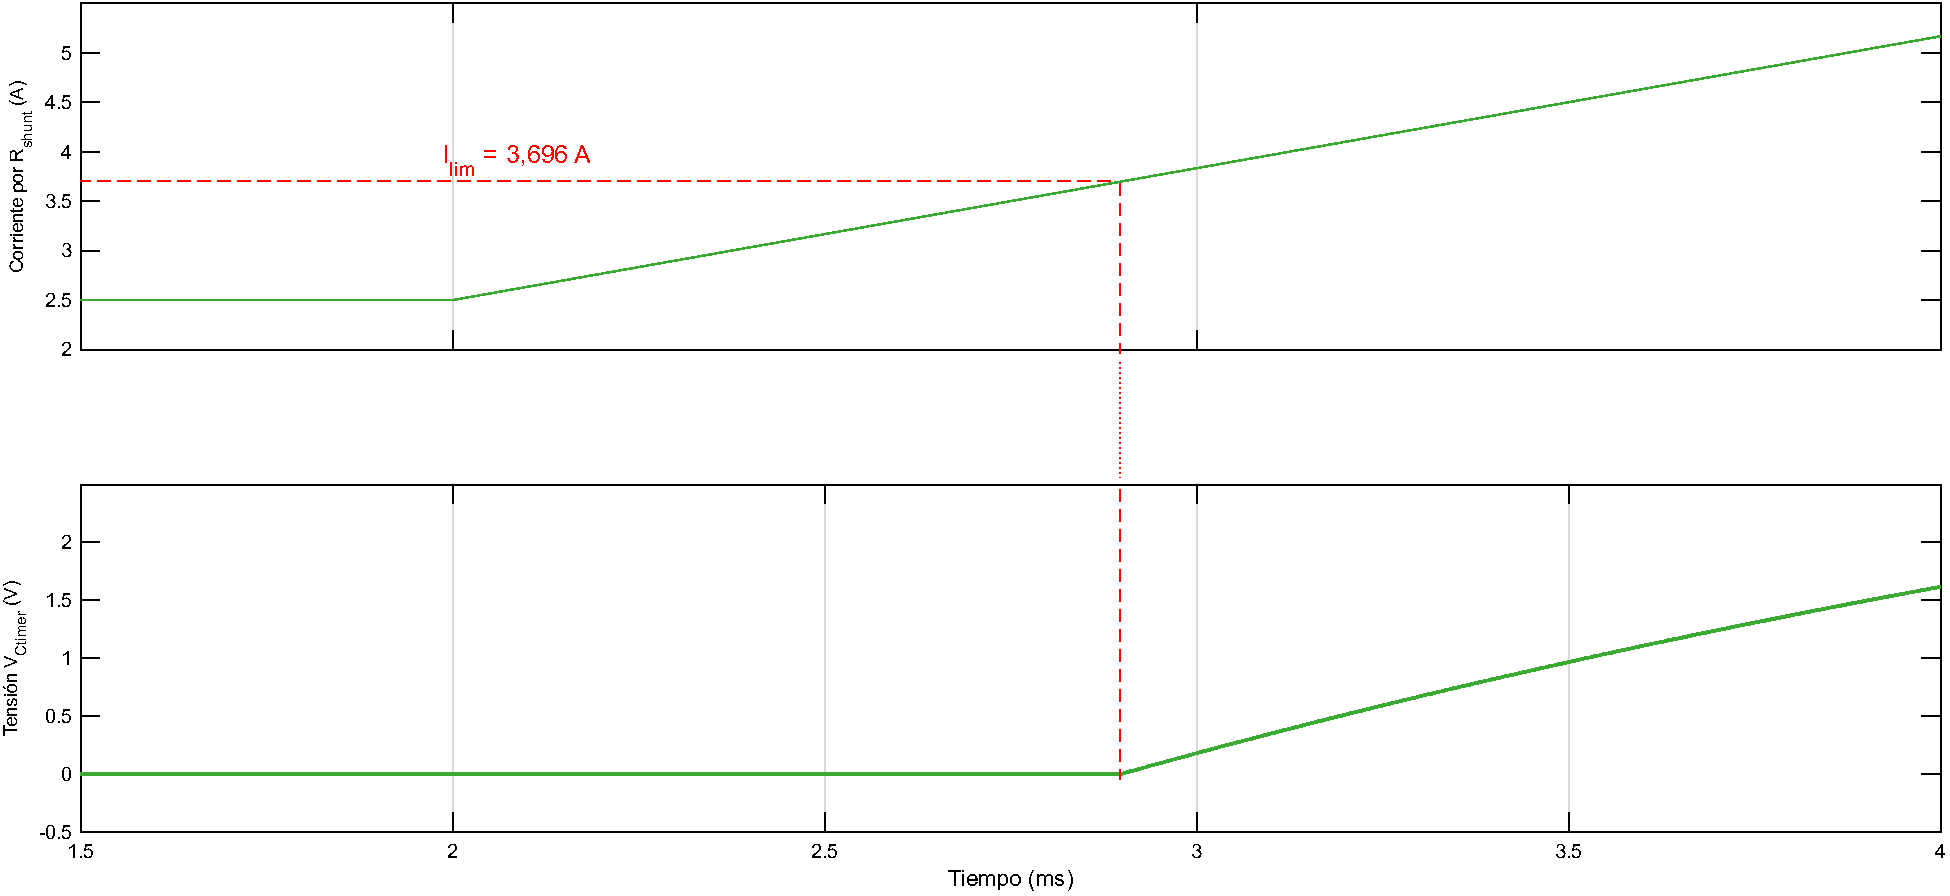
\includegraphics[width=1\textwidth]{rampa_corriente.pdf}}
    \vspace{2mm}
    {\raggedleft \textbf{Fuente:} Elaboración propia en MATLAB a partir de los resultados obtenidos en PSIM. \par}
\end{figure}

\subsubsection{Sincronización de la lógica de control}
\label{subsubsec:logica_control}
Finalmente, la Figura~\ref{fig:IvsVgsvsEntradasAND} muestra la coordinación entre la lógica digital (referenciada a masa de control), el voltaje de excitación del MOSFET y la presencia o ausencia de sobrecorriente por la resistencia de medida. 

En la figura se observan tres etapas funcionales distinguibles: el funcionamiento nominal, la limitación de corriente y el enclavamiento. 
\begin{itemize}
    \item \textbf{Funcionamiento nominal ($\text{t}<1\text{ms}$ y $2{,}1\text{ ms}<\text{t}<4\text{ ms}$):} durante estos periodos de tiempo la corriente es menor del límite establecido ($3{,}696~\text{A}$) por lo que el condensador de temporización no está cargado (salida del temporizador alta) y la corriente no incumple los límites de histéresis (salida del biestable alta). Debido a esto, la salida de la puerta lógica \textit{AND} es un ``1'' lógico y, por tanto, el \textit{driver} hace que haya una tensión $V_{\text{GS}}\text{ de } 15 V$ que provoca que el el N-MOS conduzca.
    \item \textbf{Limitación de corriente ($1\text{ ms}<\text{t}<2{,}1\text{ ms}$ y $4\text{ ms}<\text{t}<4{,}6\text{ ms}$):} durante estos periodos de tiempo la corriente se encuentra por encima del límite de $3{,}696~\text{A}$. Debido a que el tiempo de limitación es todavía menor al tiempo de \textit{trip-off}, el condensador no está cargado y la señal del temporizador se mantiene alta. Sin embargo, la señal de salida del biestable alterna ``1'' lógicos (aumento de corriente) y  ``0'' lógicos (caída de corriente) durante el tiempo de conducción ($T_{\text{on}}$) y corte ($T_{\text{off}}$) del MOSFET. De esta manera, la salida de la puerta lógica \textit{AND} es solo alta durante el aumento de corriente hasta el límite superior de histéresis y $V_{\text{GS}}$ solo será 15 voltios durante estos instantes.
    \item \textbf{Enclavamiento ($\text{t}>4{,}6\text{ ms}$): }a partir de este instante, el voltaje en el condensador $C_{\text{timer}}$ es mayor a la referencia establecida para los $1{,}5~\text{ms}$ y la señal de salida del temporizador pasa a ser baja. Debido a esto, la salida de la puerta \textit{AND} será constantemente baja y el \textit{driver} dejará de suministrar $+ 15$ voltios flotantes a la puerta del transistor, impidiendo el paso de corriente y aislando la carga.
\end{itemize}
\begin{figure}[H]
    \centering
    \fontsize{10}{12}\selectfont 
    \ffigbox[\FBwidth]
    {   \caption[Simulación de lógica de control del LCL conmutado]{Comparativa de la corriente de potencia, la tensión de puerta ($V_\text{GS}$) y los niveles lógicos de control del sistema, las salidas del biestable y del temporizador.}
        \label{fig:IvsVgsvsEntradasAND}}
    {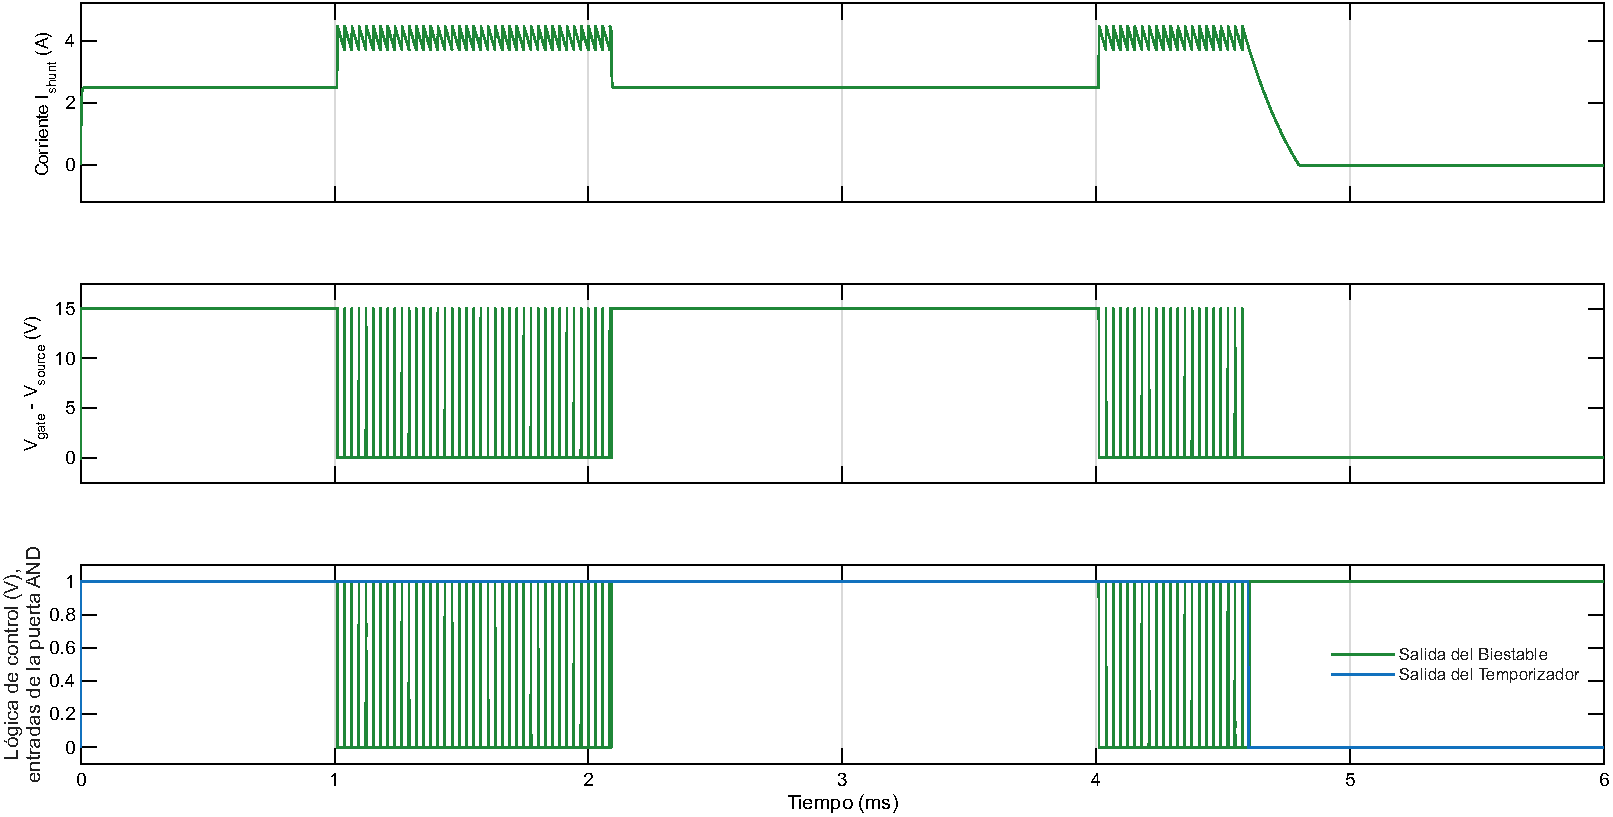
\includegraphics[width=1\textwidth]{IvsVgsvsEntradasAND.pdf}}
    \vspace{2mm}
    {\raggedleft \textbf{Fuente:} Elaboración propia en MATLAB a partir de los resultados obtenidos en PSIM. \par}
\end{figure}

\chapter{Montaje en placa, respuesta en osciloscopio y discusión de resultados}
\label{ch:montaje_y_resultados}
Tras el modelado, selección de componentes y validación con simulación en PSIM (empleando parámetros parásitos), este capítulo aborda el prototipado físico y la validación del limitador de enclavamiento conmutado mediante pruebas en el laboratorio.

Entrados en esta fase, el comportamiento del sistema deja de estar gobernado únicamente por las ecuaciones ideales expuestas y pasa a estar condicionado por la geometría del sistema, como las inductancias parásitas de las trazas de  cobre, el acoplamiento de señales, los tiempos de retraso... por lo que es el objetivo de este capítulo demostrar la viabilidad del limitador diseñado, evaluando la robustez y tiempo de respuesta frente a sobrecorrientes en un entorno de laboratorio. 

En un primer lugar se mostrará la distribución de los componentes en la placa, el uso de planos de masa... para posteriormente estudiar la respuesta en el osciloscopio de las ondas principales. Finalemente, se realizará un análisis de los resultados comparándolos con las simulaciones y justifiando las desviaciones respecto al modelo teórico. 
\section{Diseño y montaje del circuito impreso (PCB)}

El diseño de la placa de circuito impreso se ha realizado mediante la herramienta KiCad. Debido a la alta frecuencia de conmutación (en torno a los $600\text{ kHz}$) y los niveles de potencia significativos, el \textit{layout} no solo cumple con la función de conectar los componentes, sino que debe estar acortde al comportamiento dinámico y el ruido electromagnético que se pueda generar. 

A continuación, se detallan los criterios de diseño aplicados para la distribución de componentes, dimensionamiento de pistas y separación de planos de masa.

\subsection{Estrategia de distribución y agrupación}

Con el objetivo de mitigar el acoplamiento del ruido desde la etapa de potencia a la etapa de acondicionamiento se ha tenido especial cuidado con la distribución espacial de la placa. Todo el lazo analógico (acondicionamiento, temporización e histéresis) se ha agrupado de forma compacta en una zona de la PCB, separando este bloque de la zona de alta corriente. 

La agrupación del lazo se realiza por dos motivos principales causados por la zona de alta frecuencia:
\begin{itemize}
    \item \textbf{Minimización de pistas:} las trazas de entrada a los integrados actúan como antenas de los campos eléctricos ($dv/dt$) generados por la conmutación del N-MOS. Al reducir las distancias entre los componentes se reduce el acoplo de ruido y se mejoran las mediciones.
    \item \textbf{Reducción del área de los bucles de señal:} los lazos de control se trazan de forma reducida para evitar en este caso el acoplamiento magnético por inducción ($di/dt$), provocando disparos indeseados del transisotr o distorisión en la lectura de corriente. 
\end{itemize}

% ==========================================
% INSERCIÓN DE IMAGEN 1: VISTA GENERAL DEL LAYOUT
% ==========================================
\begin{figure}[H]
    \centering
    \fontsize{10}{12}\selectfont 
    
    % Inicio del bloque de subfiguras lado a lado
    \begin{subfloatrow}
        \ffigbox[\FBwidth]
        {   \caption{Vista general 2D del diseño de la PCB en KiCad.}
            \label{fig:PCB_dibujo}} % Etiqueta para citar la subfigura A
        {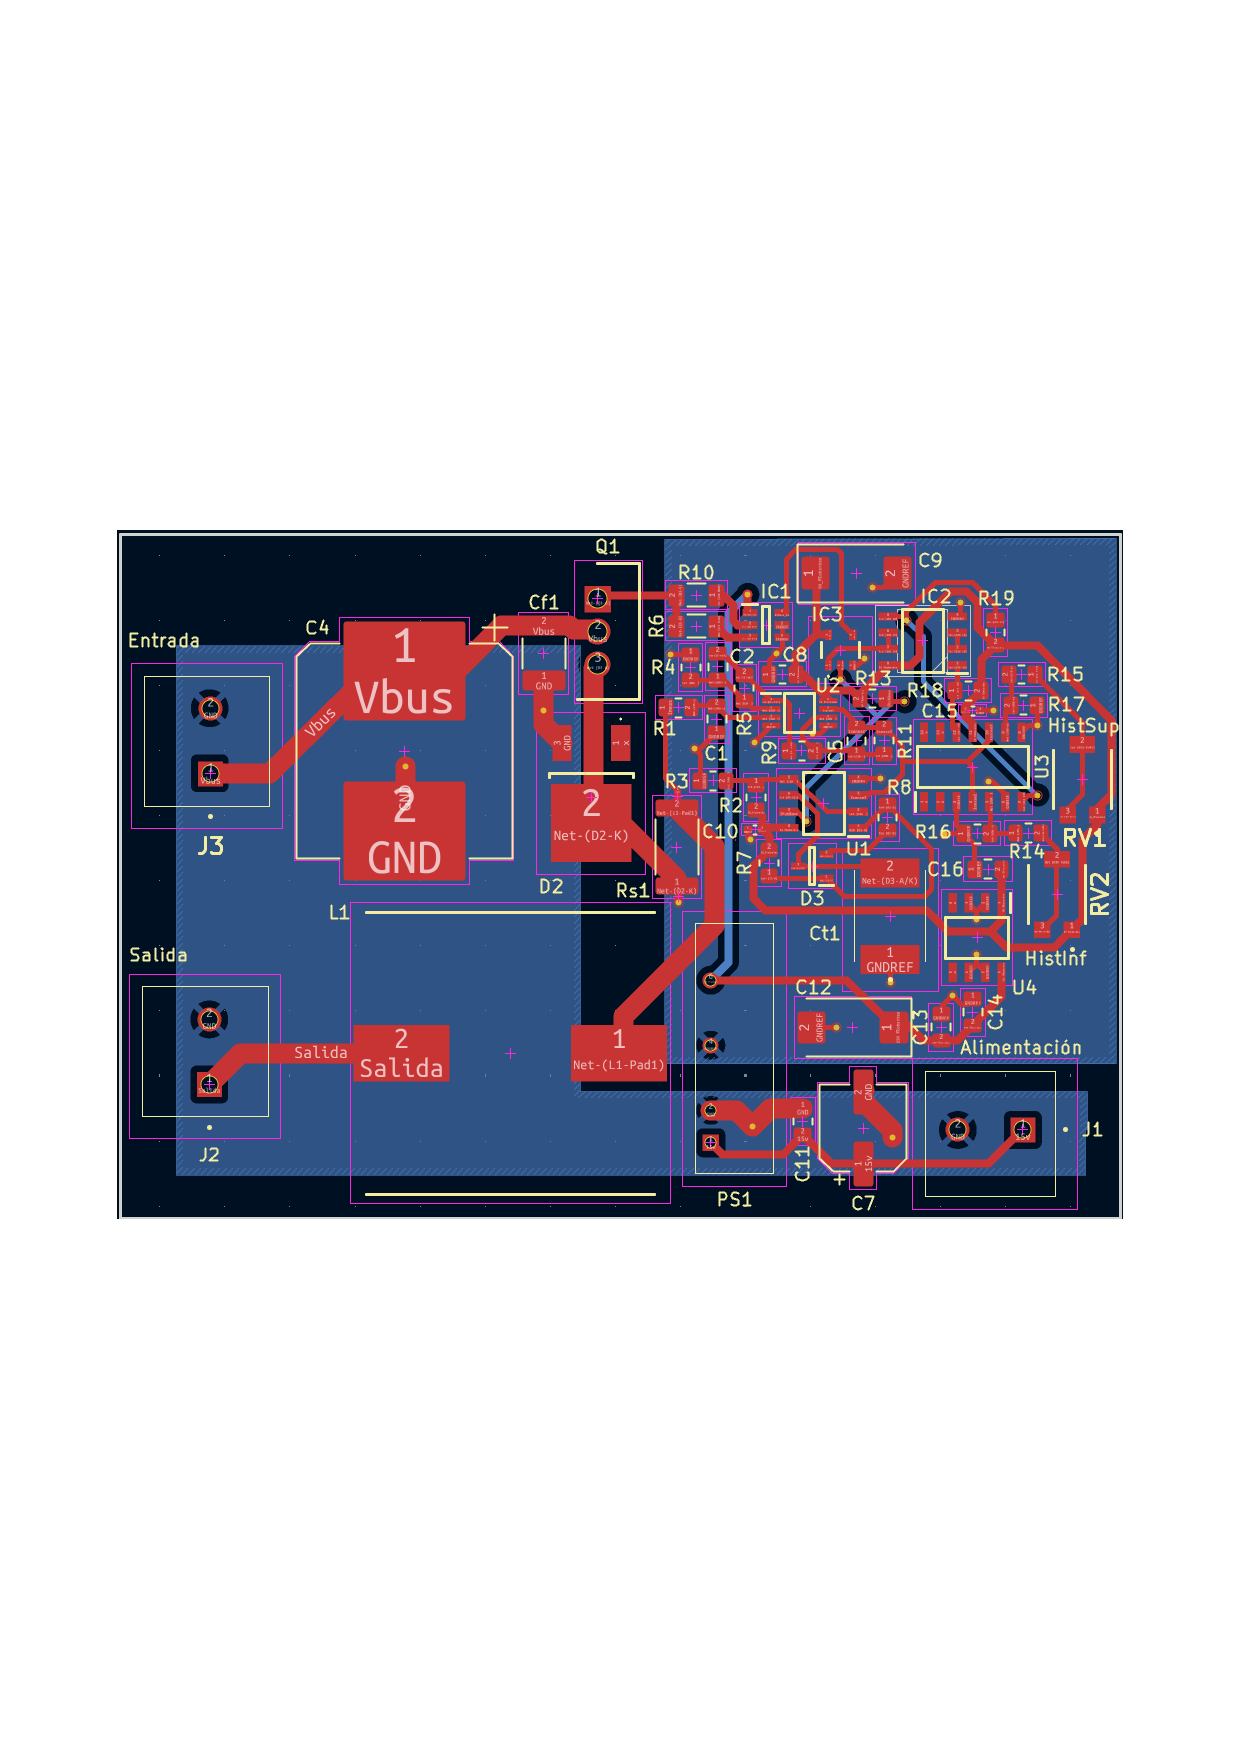
\includegraphics[width=0.45\textwidth]{PCB_dibujoFallo.pdf}} % Cambiar por tu archivo
        
        \ffigbox[\FBwidth]
        {   \caption{Vista general 3D del diseño de la PCB en KiCad (componentes comerciales).}
            \label{fig:PCB_placa}} % Etiqueta para citar la subfigura B
        {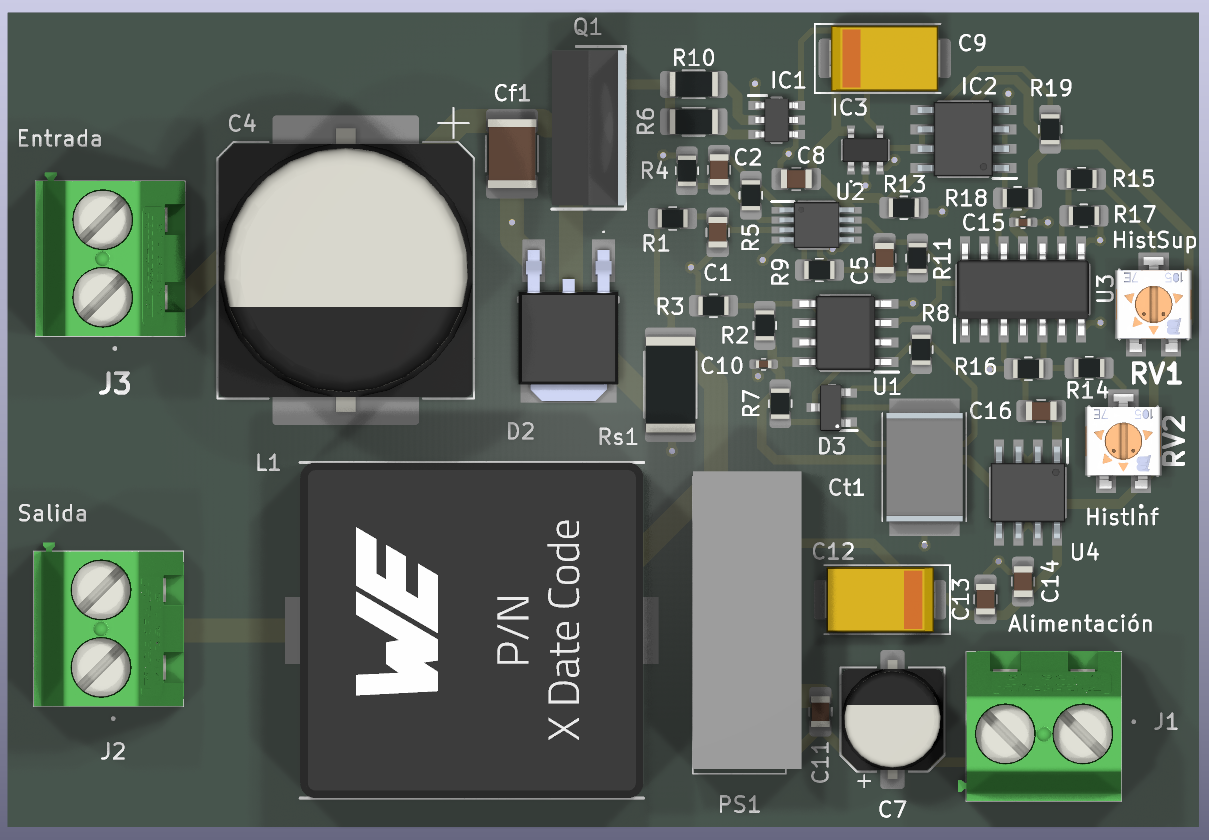
\includegraphics[width=0.45\textwidth]{PCB_POTENCIOMETRO.png}} % Cambiar por tu archivo
    \end{subfloatrow}
    % Fin del bloque de subfiguras
    
    \vspace{4mm} % Espaciado antes de la leyenda general
    
    % Leyenda general de todo el conjunto
    \caption{Vista general del diseño de la PCB en KiCad, en 2D y 3D.}
    \label{fig:PCB_dibujo} % Etiqueta para citar la figura completa
    
    \vspace{2mm}
    {\raggedleft \textbf{Fuente:} Elaboración propia en KICAD. \par}
\end{figure}


\begin{comment}
\begin{figure}[H]
    \centering
    \fontsize{10}{12}\selectfont 
    \ffigbox[\FBwidth]
    {   \caption{Vista general del diseño de la PCB en KiCad (capas de cobre y distribución segregada de los bloques de potencia y control).}
        \label{fig:PCB_dibujo}}
    {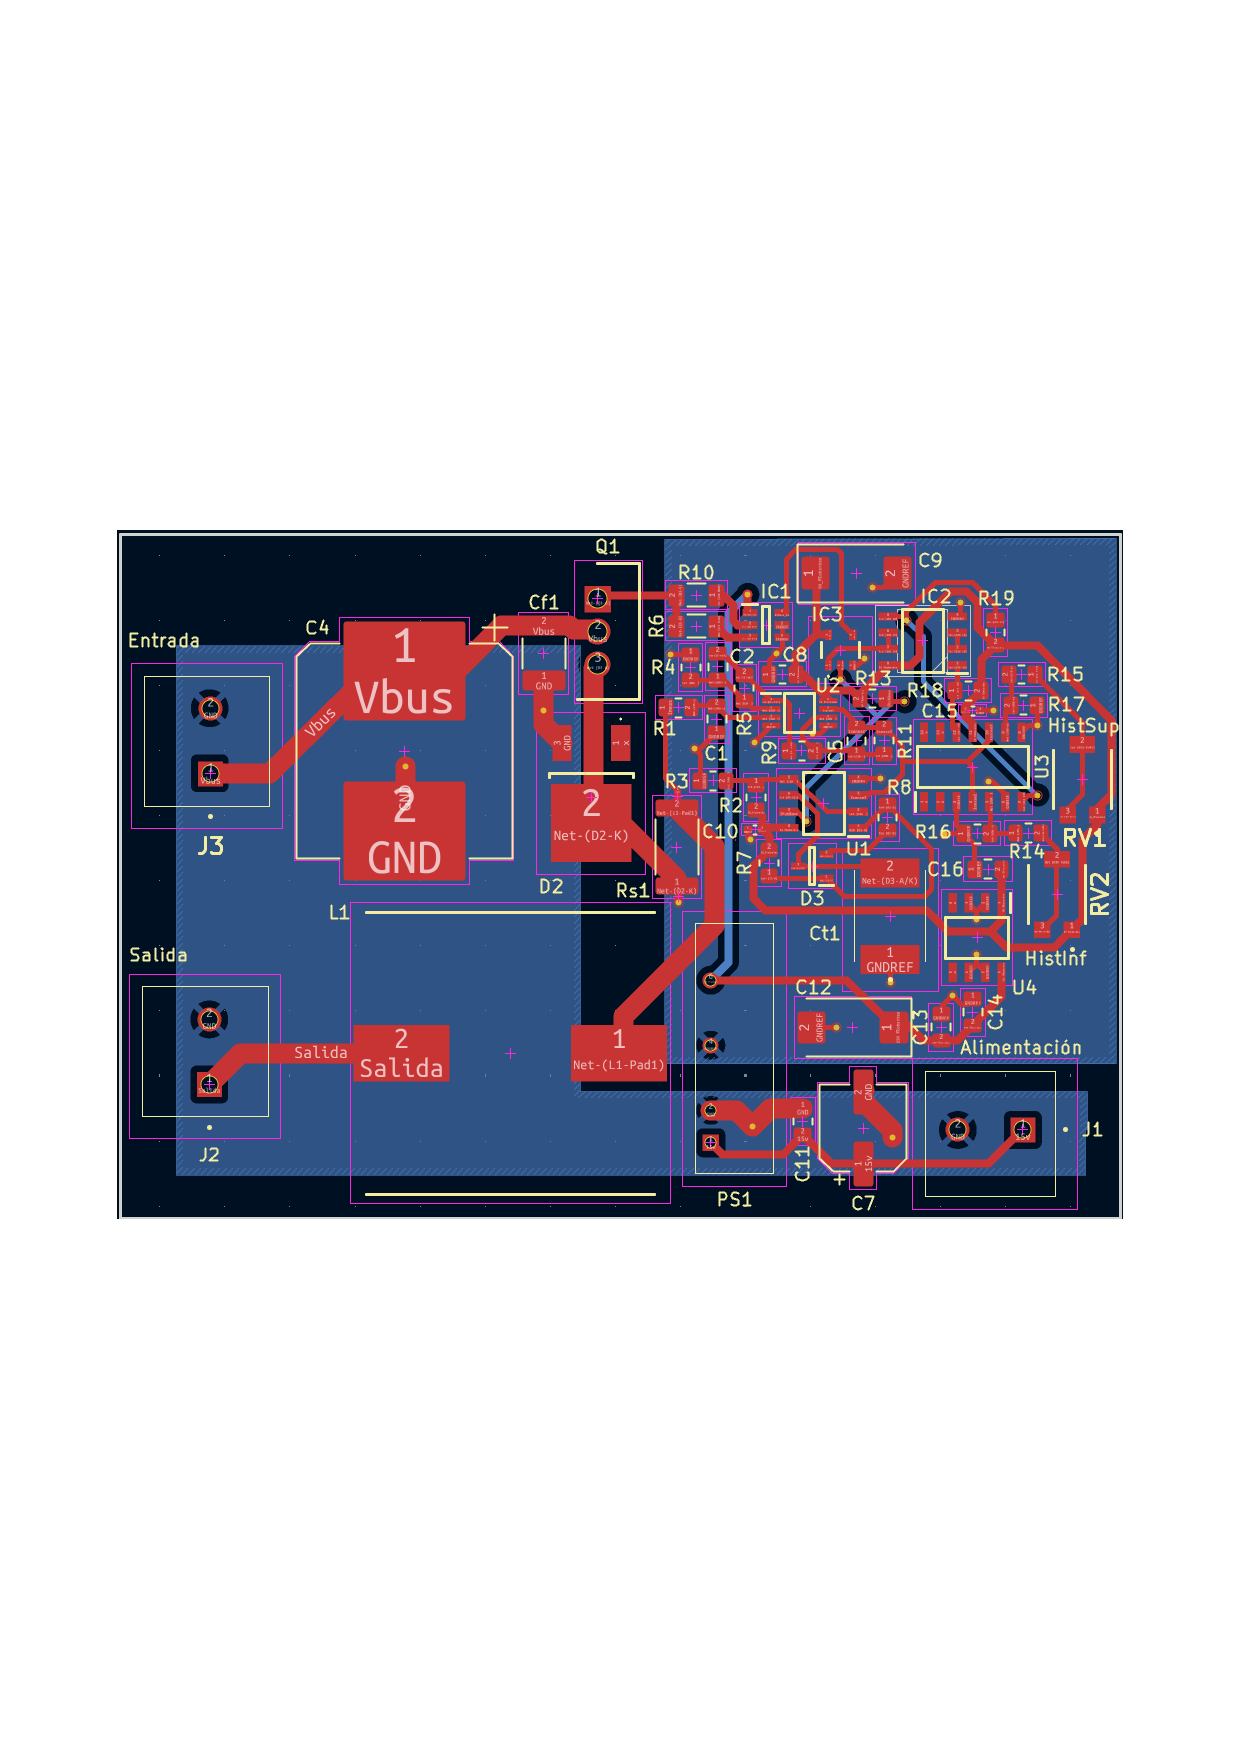
\includegraphics[width=0.8\textwidth]{PCB_dibujoFallo.pdf}}
    \vspace{2mm}
    {\raggedleft \textbf{Fuente:} Elaboración propia en KICAD. \par}
\end{figure}
\end{comment}
\subsection{Segregación y distancia entre la masa flotante de potencia y la masa del sistema}

La gestión de las masas en el circuito se realiza mediante dos planos: un plano de la masa global del sistema ($\approx0\text{ V}$) y un plano de la masa flotante del sistema (valor de la fuente del transitor), referencia que emplean los integrados como alimentación negativa. 

Debido a la diferencia de voltaje entre ambos planos, la cual puede ser de hasta $100\text{ V}$, es necesario diseñarlos manteniendo una distancia (\textit{clearance}) entre ellos de al menos $1.5\text{ mm}$, valor justificado por los siguientes motivos:
\begin{itemize}
    \item \textbf{Inmunidad frente a transitorios comunes:} durante los cambios de voltaje del plano flotante en la conmutación se producen pendientes elevadas de voltaje. Debido a la presencia de dos planos en paralelo se produce una capacidad parásita ($C = \varepsilon \frac{A}{d}$) que provocaría una inyección de corriente que podría saturar o inestabilizar el sistema. Un valor de $1.5\text{ mm}$ es un \textit{trade-off} coherente entre la disminución de la capacitancia y un tamaño correcto de la placa. 
    
    \item \textbf{Margen dieléctrico por sobretensiones (\textit{Ringing}):} Aunque nominalmente la rigidez del aire para $100\text{ V}$ requiere apenas $0.6\text{ mm}$ según la norma IPC-2221C~\cite{ipc_association_connecting_electronics_industries_generic_nodate}, las inductancias de los componentes provocan picos que superan dicha tensión. La separación garantiza un margen de seguridad robusto contra arcos eléctricos en el laboratorio.
\end{itemize}

\subsection{Dimensionamiento y capacidad de corriente de las pistas de potencia}

Las pistas conductoras, tanto de la etapa de potencia como de alimentación, se han dimensionado bajo los criterios de la norma IPC-2221C ~\cite{ipc_association_connecting_electronics_industries_generic_nodate} (\textit{Generic Standard on Printed Board Design}).
La corriente por las pistas genera pérdidas térmicas por efecto Joule por lo que una densidad de corriente alta podría aumentar la temperatura de la placa excesivamente, dañando tanto los componentes como la placa en si. 

Para mitigar este riesgo, se ha limitado la variación de temperatura a $\Delta T = 20^\circ\text{C}$ respecto al ambiente y se ha empleado el valor un valor estándar de $1\text{ oz}$ ($1{,}37\text{ mil}$) para calcular el ancho mínimo requerido para las pistas.
% ==========================================
% INSERCIÓN DE IMAGEN 2: DETALLE DE ANCHOS DE PISTA
% ==========================================
\begin{figure}[H]
    \centering
    \fontsize{10}{12}\selectfont 
    \ffigbox[\FBwidth]
    {   \caption{Dimensionamiento del ancho de las pistas de alta corriente para el cumplimiento de los márgenes térmicos de la norma IPC-2221.}
    \label{fig:ancho_pistas}}
    {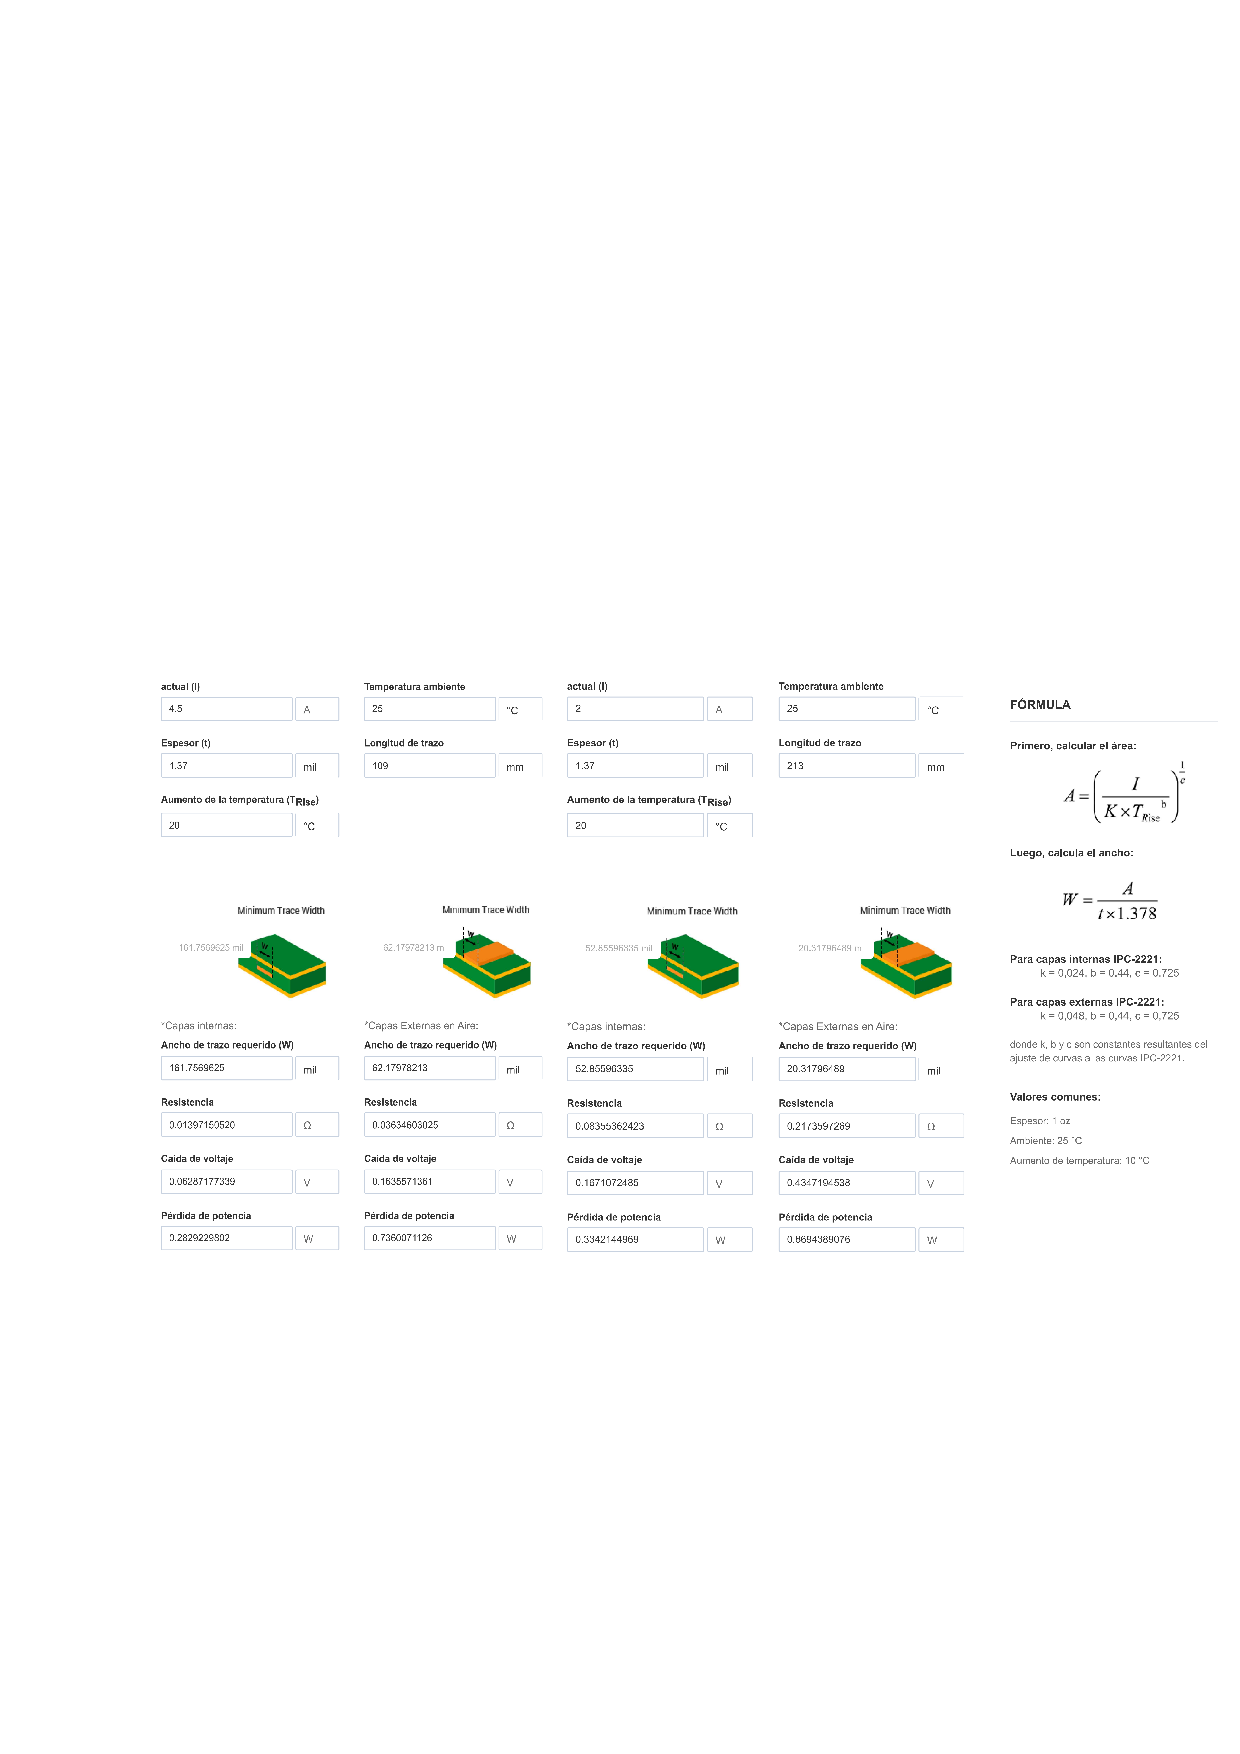
\includegraphics[width=0.8\textwidth]{AnchoVias.pdf}}
    \vspace{2mm}
    {\raggedleft \textbf{Fuente:} Elaboración propia a partir de la calculadora de anchos de vía de \textit{PCBWay} \cite{noauthor_calculadora_nodate}. \par}
\end{figure}

A partir de los resultados de la Figura~\ref{fig:ancho_pistas}, se han empleados anchos de $64\text{ mil}$ para las pistas de la etapa de potencia, y ancho de $25\text{ mil}$ para las alimentaciones de $15\text{ V}$ y las señales de control de mayor corriente como es el caso de la salida del \textit{driver}. Para las señales de control de baja corriente entre integrados se emplean pistas de $15\text{ mil}$.
\subsection{Colocación estratégica de condensadores de desacoplo}
Un aspecto a tener en cuenta en la distribución para la integridad de las señales y la estabilidad de las mismas es el posicionamiento de los condensadores de desacoplo cerámicos asocidados a los circuitos integrados y al transisor. 

Tanto para los comparadores, el OPAMP, las puertas lógicas, el \textit{driver},... como para el drenador del transistor de potencia, los condensadores de desacoplo se han colocado próximos a los pines de alimentación ($V_{CC}$ y $GND$), minimizando la distancia física. 
% ==========================================
% INSERCIÓN DE IMAGEN 3 Y 4: DETALLES DE DESACOPLO / KICAD ROUTING
% ==========================================
\begin{figure}[H]
    \centering
    \fontsize{10}{12}\selectfont 
    \ffigbox[\FBwidth]
    {   \caption{Compactacion de la zona de control en la PCB.}
    \label{fig:detalles}}
    {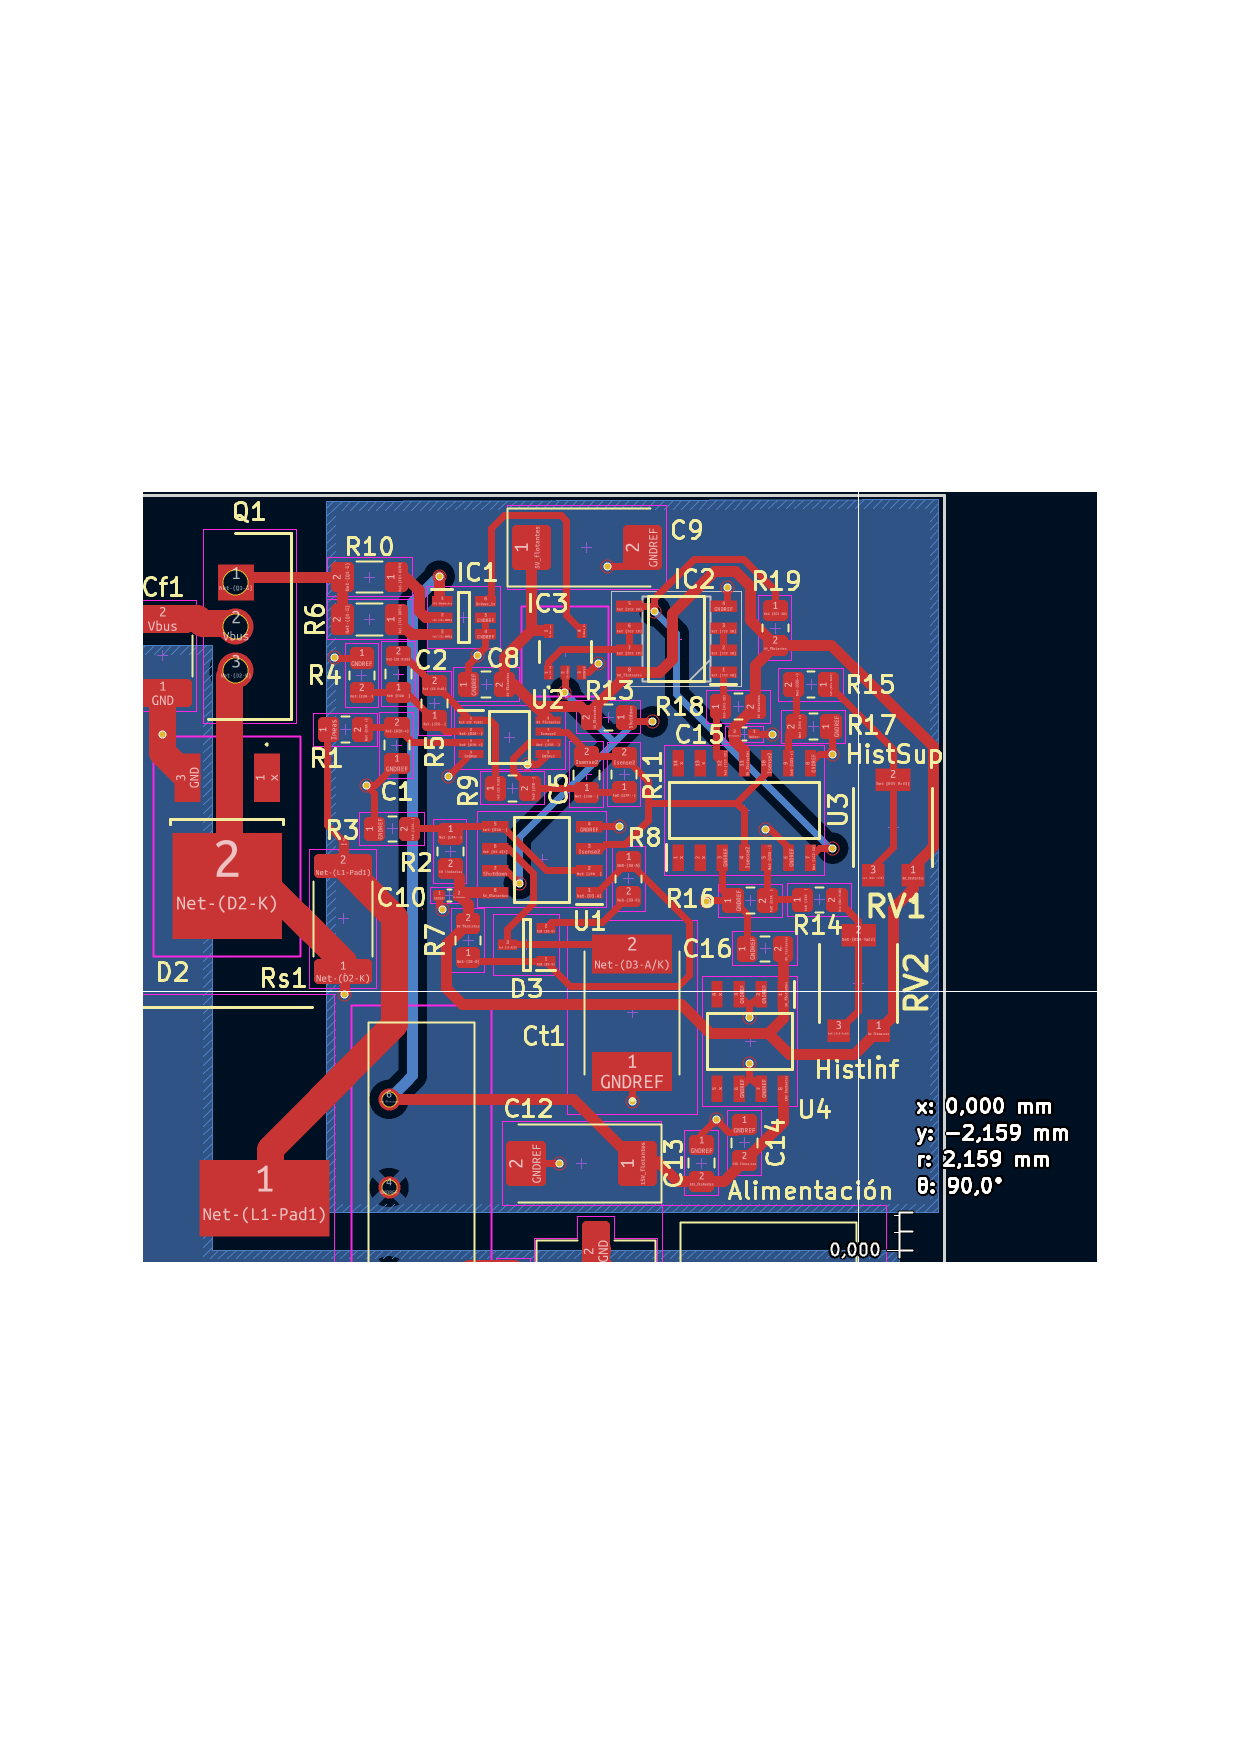
\includegraphics[width=0.8\textwidth]{Regla.pdf}}
    \vspace{2mm}
    {\raggedleft \textbf{Fuente:} Elaboración propia en KICAD.  \par}
\end{figure}
La justificación teórica de esta disposición (ilustrada en la Figura~\ref{fig:detalles}) se encuentra, al igual que anteriormente, en contrarrestar la inductancia parásita de las trazas de la PCB ($L_{traza} \approx 1\text{ nH/mm}$). A alta frecuencia de conmutación los milimetros de pista añaden impedancias que provocarían caídas de tensión locales, por lo que la cercanía de los condensadores permitiría suministrar los picos de corriente necesarios, filtrar el ruido de alta corriente y eliminar las caídas de tensión mencionadas. 
\begin{comment}
script o excel ??? 
Valores necesarios para cambiar el trip-off time, la banda de histéresis y el valor de limitación
-Divisor hist superior
-Divisor hist inferior
-Referencia TimON
-Red RC temporización


Una vez tenemos una arquitectura correcta en cuanto a perdidas, limites de histéresis, a una frecuencia controlable pero que limite las pérdidas y hemos sido capaces de ajustar la limitación a nuestro tiempo buscado el siguiente objetivo debe ser encontrar una manera de adaptar nuestro circuito a distintos:
-Corrientes de limitación: estamos limitando a 3.7 pero para otro proyecto podemos querer hacerlo a 5.1 o a 7.3
- Trip-off time: en nuestro caso se ha sido conservativo con el tiempo de limitación por la falta de regulación en espacio (clases ecss ) para los 100 voltios y ser un diseño genérico sin una idea concreta de cual será la carga para la que se prepara el circuito. Es por tanto un trabajo que tiene como objetivo optimizar el diseño y entender los cambios necesarios para adaptarlo. 
- Limites de histéresis: según también las limitaciones, senisbilidad... de la carga debemos poder adaptar a nuestro gusto los límites de histéresis de nuestro circuito. Para ello debemos poder tanto seleccionar unos valores determinado (para una limitacion de 5.1 un valor de hyst entre 5.1 y 5.7) o un porcentaje por arriba y por abajo permisible.

Una vez tenemos estos valores podemos modificar nuestro circuito. Manteniendo la topología podremos modificar ciertos valores para adaptar. 


\textbf{CAMBIOS PARA EL BLOQUE TEMPORIZADOR:}

Hay dos partes importantes en el a la hora de adaptarlo a otros tiempos:
- El condensador se empieza a cargar cuando V>Vshunt para la corriente determinado, es decir, si Ilim' = 5.7A empezará el temporizador cuando esté en la entrada 5.7*0.022*25 = 3.135V. Por tanto debemos cambiar el divisor de resistencias que hacen la referencia. Esto es necesario para el CAMBIO DE ILIM

- A partir de la alimentación de 5V, la red RC es la que marca el tiempo de temporización de nuestro circuito. Por tanto, debemos cambiar el valor de la red RC (R PULL UP Y CONDENSADOR DE CARGA) ajustandolo al nuevo valor. Esto es necesario para el CAMBIO DE TRIP-OFF TIME



\textbf{CAMBIOS PARA EL SENSOR DE CORRIENTE:}
Debido a que el único objetivo del mismo es la amplificación de la señal medida en el circuito con una ganancia de 25 V/V, podemos mantener este valor y reemplear directamente este circuito. 


\textbf{CAMBIOS PARA EL BLOQUE DE HISTÉRESIS:}

Hay dos partes: limite inferior y limite superior.

Hay que modificar los divisores de tensión tanto superior como inferior para que esté adaptado a los valores de histéresis que buscamos. Esto es necesario para el CAMBIO DE LÍMITES DE HISTÉRESIS

Además, para el cambio de cualquoiera de los parámetros debe tenerse en cuenta las especificaciones de los integrados y determinar si los nuevos valores no los rompen.
\end{comment}
\begin{bloqueRevisar}
    

\chapter{Metodología de Escalado del Diseño}

Una vez validada la arquitectura del limitador de corriente de enclavamiento (LCL) conmutado en términos de eficiencia, respuesta transitoria y márgenes de estabilidad térmica para el punto de operación de consigna, el diseño se sistematiza como una plataforma modular. El objetivo de este capítulo es definir el procedimiento analítico para adaptar el circuito a diferentes escenarios operacionales, caracterizados por nuevas tensiones de bus ($V_{bus}$), corrientes de limitación ($I_{lim}$), límites de histéresis ($\Delta i$) y tiempos de disparo (\textit{trip-off time}, $t_{trip}$).

Para automatizar este proceso, se ha desarrollado un script de cálculo sencillo(cuyo código fuente se adjunta en el Anexo) que recibe las especificaciones de la nueva carga y computa de forma secuencial tanto las restricciones mecánicas y magnéticas de la etapa de potencia como los componentes pasivos de la lógica analógica de control.

\section{Dimensionado y Validación de la Etapa de Potencia}

El escalado del circuito no puede limitarse a la modificación de los umbrales de control; un cambio en las especificaciones modifica el estrés térmico y magnético de los componentes de potencia:

\begin{itemize}
    \item \textbf{Resistencia de sensado ($R_{shunt}$):} La potencia disipada por efecto Joule en régimen nominal viene dada por $P_{shunt} = I_{nom}^2 \cdot R_{shunt}$. Al elevar la corriente nominal del proyecto, se debe verificar que $P_{shunt}$ no supere la potencia nominal del componente físico (fijada en $0.5$~W en el prototipo actual). En caso de excederse, la metodología exige disminuir el valor óhmico de $R_{shunt}$ o seleccionar un encapsulado de mayor disipación, teniendo en cuenta que cualquier modificación en $R_{shunt}$ altera la tensión acondicionada según la relación $V_{sense} = I_L \cdot R_{shunt} \cdot G$.
    \item \textbf{Saturación de la inductancia ($L$):} Se debe asegurar que la corriente máxima del ciclo de histéresis ($I_{hys,sup}$) junto al sobrepaso dinámico inicial (\textit{overshoot}) no alcancen la corriente de saturación ($I_{sat}$) del núcleo magnético seleccionado, evitando la pérdida de linealidad y un crecimiento exponencial de la corriente.
    \item \textbf{Estrés térmico del MOSFET:} Las pérdidas por conducción del transistor ($P_{cond} = R_{DS,ON} \cdot I_{rms}^2$) crecen de forma cuadrática con la corriente. Utilizando el modelo térmico equivalente del sistema, el script valida que la temperatura de la unión no exceda el límite de seguridad establecido ($T_{j,max} = 125^\circ$C):
    \begin{equation}
        T_j = T_a + (P_{cond} + P_{sw}) \cdot (R_{\theta,JC} + R_{\theta,CS} + R_{\theta,SA}) \le 125^\circ\text{C}
    \end{equation}
\end{itemize}

\section{Modificaciones en el Bloque Temporizador de Seguridad}

El bloque de temporización requiere dos ajustes independientes para su correcto escalado:

\begin{enumerate}
    \item \textbf{Referencia de activación ($V_{TimON}$):} Para asegurar que el temporizador comience a acumular carga únicamente cuando la corriente supera el valor de limitación nominal $I_{lim}$, se debe recalcular el divisor resistivo ($R_1$ y $R_2$) alimentado a $5$~V que fija la tensión de referencia:
    \begin{equation}
        V_{TimON} = I_{lim} \cdot R_{shunt} \cdot G
    \end{equation}
    Donde $G = 25$~V/V es la ganancia de la etapa de acondicionamiento. A partir de $V_{TimON}$, la relación del divisor viene dada por:
    \begin{equation}
        \frac{R_1}{R_2} = \frac{5\,\text{V}}{V_{TimON}} - 1
    \end{equation}
    \item \textbf{Red RC de temporización asimétrica:} El tiempo de disparo (\textit{trip-off time}, $t_{trip}$) viene determinado por la constante de tiempo de carga $\tau_{carga} = R_3 \cdot C_{timer}$. Fijando el condensador en un valor comercial estable ($C_{timer} = 100$~nF), la resistencia de carga $R_3$ se calcula mediante la ecuación transitoria de carga considerando la caída del diodo ($V_F \approx 0.32$~V):
    \begin{equation}
        R_3 = \frac{-t_{trip}}{C_{timer} \cdot \ln\left(1 - \frac{V_{TimON}}{5\,\text{V} - V_F}\right)}
    \end{equation}
\end{enumerate}

\section{Modificaciones en el Bloque de Histéresis}

Para adaptar los límites de conmutación a la nueva banda permisible de la carga, se deben modificar las tensiones de referencia de los comparadores rápidos ($V_{superior}$ y $V_{inferior}$):

\begin{itemize}
    \item \textbf{Umbral superior:} $V_{superior} = I_{hys,sup} \cdot R_{shunt} \cdot G$
    \item \textbf{Umbral inferior:} $V_{inferior} = I_{hys,inf} \cdot R_{shunt} \cdot G$
\end{itemize}
Estas referencias flotantes se ajustan físicamente mediante la sintonización de los divisores potenciómetricos correspondientes del bloque de histéresis analógico, asegurando que la banda de histéresis $\Delta i = I_{hys,sup} - I_{hys,inf}$ mantenga una frecuencia operacional compatible con las pérdidas dinámicas admisibles del MOSFET y la velocidad de respuesta del lazo analógico.



	% COMENZAR A ESCRIBIR la MEMORIA
	
	% IMPORTANTE: en LaTeX hay una serie de caracteres especiales, que son: # $ % & \ ^ _ { } ~. Si aparecen en el texto, tendrás un error al compilar. La mayoría se pueden escapar escribiendo \ delante. Para \ utiliza \textbackslash ; para ^ \textasciitilde y para ~ \textasciicircum.

    % COMO incluir una FIGURA siguiendo las recomendaciones de la Guía: Alineación del título: izquierda, en la parte inferior de la figura; fuente a 10pt (el resto de la memoria está a 12); Numeración de la figura: se identificarán con números arábigos consecutivos tras la palabra Tabla. Si se sigue un esquema numérico de capítulos, el número de la tabla debe identificar con su primer dígito al capítulo, seguido por un punto y el número consecutivo que corresponda (Tabla 1.1, etc.); Propiedad intelectual: Se debe indicar la fuente de origen de la información en la parte inferior de la figura, a continuación del título.
    
    % EJEMPLO DE INCLUSIÓN de una figura:
    % \begin{figure}[H]
    % 	\ffigbox[\FBwidth] {
    % 	\caption[Nombre que aparecerá en el índice]{Nombre que aparecerá debajo de la figura}
    % 	}
    % 	{\includegraphics[width=0.8\textwidth]{archivo de la imagen; deberá estar en la carpeta de imágenes}}
    % \end{figure}



%\begin{figure}[H]
 %   \centering
  %  % Forzamos 10pt para cumplir con la normativa de tu guía
   % \fontsize{10}{12}\selectfont 
    %\ffigbox[\FBwidth]
    %{
     %   \caption{Gráfica de área de operación segura (SOA) para el MOSFET de canal P}
     %   \label{fig:comparativa_mosfet}
    %}
    %{
     %   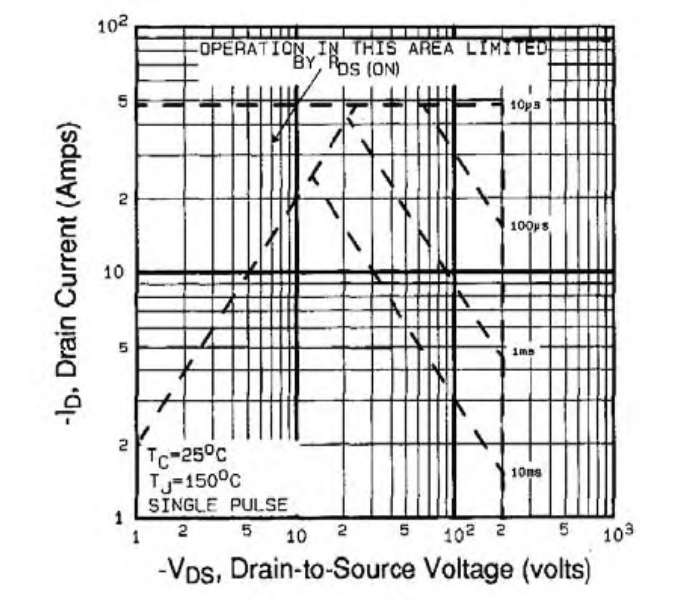
\includegraphics[width=0.8\textwidth]{SOA.png}
    %}
    
    % Añadimos la fuente requerida por tu guía de TFG
    %\vspace{2mm}
    %{\raggedleft \textbf{Fuente:} Extraído de hoja de datos del IRFP9240PBF\cite%%{vishay_semiconductors_irfp9240pbfmosfet_nodate}. \par}
%\end{figure}




    
    % COMO incluir una TABLA siguiendo las recomendaciones de la Guía: Alineación del título: Centrado en la parte superior de de la tabla, en la parte superior de la tabla; fuente a 10pt (el resto de la memoria está a 12) y en mayúsculas; Numeración: se identificarán con números arábigos consecutivos tras la palabra Tabla. Si se sigue un esquema numérico de capítulos, el número de la tabla debe identificar con su primer dígito al capítulo, seguido por un punto y el número consecutivo que corresponda (Tabla 1.1, etc.); Propiedad intelectual: Se debe indicar la fuente de origen de la información en la parte inferior de la tabla.
    
    % EJEMPLO DE INCLUSIÓN de una tabla:
% \begin{table}[H]
% 	\ttabbox[\FBwidth]
%	\centering
	%\fontsize{10}{12}\selectfont
% 	{\caption{Lorem ipsum}}
% 	{\begin{tabular}{|c|P{1.5cm}|c|P{1.5cm}|P{2cm}|c|P{1.5cm}|P{2cm}|}
% 		\hline
% 		\multicolumn{2}{|c|}{\textbf{I}} & \multicolumn{2}{c|}{\textbf{II}} & \multicolumn{3}{c|}{\textbf{III}} & \textbf{IV} \\
% 		\hline
% 		x & y & x & y & x & y & x & y \\
% 		\hline
% 		10.0 & 8.04 & 10.0 & 9.14 & 10.0 & 7.46 & 8.0 & 6.58 \\
% 		\hline
% 		8.0 & 6.95 & 8.0 & 8.14 & 8.0 & 6.77 & 8.0 & 5.76 \\
% 		\hline
% 		13.0 & 7.58 & 13.0 & 8.74 & 13.0 & 12.74 & 8.0 & 7.71 \\
% 		\hline
% 		9.0 & 8.81 & 9.0 & 8.77 & 9.0 & 7.11 & 8.0 & 8.84 \\
% 		\hline
% 		11.0 & 8.33 & 11.0 & 9.26 & 11.0 & 7.81 & 8.0 & 8.47 \\
% 		\hline
% 		14.0 & 9.96 & 14.0 & 8.10 & 14.0 & 8.84 & 8.0 & 7.04 \\
% 		\hline
% 		6.0 & 7.24 & 6.0 & 6.13 & 6.0 & 6.08 & 8.0 & 5.25 \\
% 		\hline
% 		4.0 & 4.26 & 4.0 & 3.10 & 4.0 & 5.39 & 19.0 & 12.50 \\
% 		\hline
% 		12.0 & 10.84 & 12.0 & 9.13 & 12.0 & 8.15 & 8.0 & 5.56 \\
% 		\hline
% 		7.0 & 4.82 & 7.0 & 7.26 & 7.0 & 6.42 & 8.0 & 7.91 \\
% 		\hline
% 		5.0 & 5.68 & 5.0 & 4.74 & 5.0 & 5.73 & 8.0 & 6.89 \\
% 		\hline
% 		\multicolumn{5}{l}{Fuente: BOE}
% 	\end{tabular}}
% \end{table}

%\begin{table}[H]
 %   \centering
%	\label{table:si_vs_sic}
 %   \fontsize{10}{12}\selectfont
 %   \ttabbox[\textwidth]
 %   {\caption{COMPARACIÓN DE PROPIEDADES FÍSICAS Y ELÉCTRICAS ENTRE SILICIO (SI) Y CARBURO DE SILICIO (SIC)}}
  %  {\begin{tabular}{|P{3.5cm}|P{4.5cm}|P{4.5cm}|}
        %\hline
       % \textbf{PARÁMETRO FÍSICO / ELÉCTRICO} & \textbf{SILICIO (SI)} & \textbf{CARBURO DE SILICIO (SIC, 4H-SIC)} \\
        %\hline
        %Banda prohibida ($E_g$) & $\sim 1,1$ eV & $\sim 3,2\text{--}3,3$ eV \\
        %\hline
        %Campo de ruptura máximo & $\sim 0,3$ MV/cm & $\sim 2,5\text{--}3$ MV/cm (unos $10\times$ mayor) \\
        %\hline
        %Resistencia on-state específica $R_{on}^{sp}$ & Alta, limitada por el campo & Muy baja, permite dispositivos de alta tensión pequeños \\
        %\hline
        %Conductividad térmica & $\sim 150\text{--}170$ W/(m·K)* & $\sim 370\text{--}490$ W/(m·K) \\
        %\hline
        %Temperatura máxima de trabajo & Limitada ($< 150\text{--}175$ °C) & Hasta $\sim 200\text{--}250$ °C \\
        %\hline
        %Comportamiento en alta frecuencia & Adecuado, pero con pérdidas dinámicas mayores & Diseñado para alta frecuencia y eficiencia en PWM \\
        %\hline
        %\multicolumn{3}{r}{\rule{0pt}{3ex}\textbf{Fuente:} Elaboración propia a partir de SA Materials\cite%{noauthor_carburo_nodate} }
        %\label{}
        %   \end{tabular}}
%\end{table}





%----------
%	BIBLIOGRAFÍA
%----------	

%\nocite{*} % Si quieres que aparezcan en la bibliografía todos los documentos que la componen (también los que no estén citados en el texto) descomenta está línea

\clearpage
\addcontentsline{toc}{chapter}{Bibliografía}
\setquotestyle[english]{british} % Cambiamos el tipo de cita porque en el estilo IEEE se usan las comillas inglesas.
\printbibliography



%----------
%	ANEXOS
%----------	

% Si tu trabajo incluye anexos, puedes descomentar las siguientes líneas
\chapter* {Anexo 1}
\begin{bloqueRevisar}
BILL OF MATERIALS

Revisar cuales son los componentes finales usados en la placa y preguntar que debería poner: lo que he usado para los cálculos o lo que al final se emplean realmente. 

\end{bloqueRevisar}

\pagenumbering{gobble} % Las páginas de los anexos no se numeran
\end{bloqueRevisar}


\end{document}